\documentclass[12pt,a4paper]{article}

\usepackage[a4paper,text={16.5cm,25.2cm},centering]{geometry}
\usepackage{lmodern}
\usepackage{amssymb,amsmath}
\usepackage{bm}
\usepackage{graphicx}
\usepackage{microtype}
\usepackage{hyperref}
\setlength{\parindent}{0pt}
\setlength{\parskip}{1.2ex}

\hypersetup
       {   pdfauthor = {  },
           pdftitle={ Global Sensitivity Analysis on Voriconazole model },
           colorlinks=TRUE,
           linkcolor=black,
           citecolor=blue,
           urlcolor=blue
       }

\title{ Global Sensitivity Analysis on Voriconazole model }


\date{ 2021-04-26 }

\usepackage{upquote}
\usepackage{listings}
\usepackage{xcolor}
\lstset{
    basicstyle=\ttfamily\footnotesize,
    upquote=true,
    breaklines=true,
    breakindent=0pt,
    keepspaces=true,
    showspaces=false,
    columns=fullflexible,
    showtabs=false,
    showstringspaces=false,
    escapeinside={(*@}{@*)},
    extendedchars=true,
}
\newcommand{\HLJLt}[1]{#1}
\newcommand{\HLJLw}[1]{#1}
\newcommand{\HLJLe}[1]{#1}
\newcommand{\HLJLeB}[1]{#1}
\newcommand{\HLJLo}[1]{#1}
\newcommand{\HLJLk}[1]{\textcolor[RGB]{148,91,176}{\textbf{#1}}}
\newcommand{\HLJLkc}[1]{\textcolor[RGB]{59,151,46}{\textit{#1}}}
\newcommand{\HLJLkd}[1]{\textcolor[RGB]{214,102,97}{\textit{#1}}}
\newcommand{\HLJLkn}[1]{\textcolor[RGB]{148,91,176}{\textbf{#1}}}
\newcommand{\HLJLkp}[1]{\textcolor[RGB]{148,91,176}{\textbf{#1}}}
\newcommand{\HLJLkr}[1]{\textcolor[RGB]{148,91,176}{\textbf{#1}}}
\newcommand{\HLJLkt}[1]{\textcolor[RGB]{148,91,176}{\textbf{#1}}}
\newcommand{\HLJLn}[1]{#1}
\newcommand{\HLJLna}[1]{#1}
\newcommand{\HLJLnb}[1]{#1}
\newcommand{\HLJLnbp}[1]{#1}
\newcommand{\HLJLnc}[1]{#1}
\newcommand{\HLJLncB}[1]{#1}
\newcommand{\HLJLnd}[1]{\textcolor[RGB]{214,102,97}{#1}}
\newcommand{\HLJLne}[1]{#1}
\newcommand{\HLJLneB}[1]{#1}
\newcommand{\HLJLnf}[1]{\textcolor[RGB]{66,102,213}{#1}}
\newcommand{\HLJLnfm}[1]{\textcolor[RGB]{66,102,213}{#1}}
\newcommand{\HLJLnp}[1]{#1}
\newcommand{\HLJLnl}[1]{#1}
\newcommand{\HLJLnn}[1]{#1}
\newcommand{\HLJLno}[1]{#1}
\newcommand{\HLJLnt}[1]{#1}
\newcommand{\HLJLnv}[1]{#1}
\newcommand{\HLJLnvc}[1]{#1}
\newcommand{\HLJLnvg}[1]{#1}
\newcommand{\HLJLnvi}[1]{#1}
\newcommand{\HLJLnvm}[1]{#1}
\newcommand{\HLJLl}[1]{#1}
\newcommand{\HLJLld}[1]{\textcolor[RGB]{148,91,176}{\textit{#1}}}
\newcommand{\HLJLs}[1]{\textcolor[RGB]{201,61,57}{#1}}
\newcommand{\HLJLsa}[1]{\textcolor[RGB]{201,61,57}{#1}}
\newcommand{\HLJLsb}[1]{\textcolor[RGB]{201,61,57}{#1}}
\newcommand{\HLJLsc}[1]{\textcolor[RGB]{201,61,57}{#1}}
\newcommand{\HLJLsd}[1]{\textcolor[RGB]{201,61,57}{#1}}
\newcommand{\HLJLsdB}[1]{\textcolor[RGB]{201,61,57}{#1}}
\newcommand{\HLJLsdC}[1]{\textcolor[RGB]{201,61,57}{#1}}
\newcommand{\HLJLse}[1]{\textcolor[RGB]{59,151,46}{#1}}
\newcommand{\HLJLsh}[1]{\textcolor[RGB]{201,61,57}{#1}}
\newcommand{\HLJLsi}[1]{#1}
\newcommand{\HLJLso}[1]{\textcolor[RGB]{201,61,57}{#1}}
\newcommand{\HLJLsr}[1]{\textcolor[RGB]{201,61,57}{#1}}
\newcommand{\HLJLss}[1]{\textcolor[RGB]{201,61,57}{#1}}
\newcommand{\HLJLssB}[1]{\textcolor[RGB]{201,61,57}{#1}}
\newcommand{\HLJLnB}[1]{\textcolor[RGB]{59,151,46}{#1}}
\newcommand{\HLJLnbB}[1]{\textcolor[RGB]{59,151,46}{#1}}
\newcommand{\HLJLnfB}[1]{\textcolor[RGB]{59,151,46}{#1}}
\newcommand{\HLJLnh}[1]{\textcolor[RGB]{59,151,46}{#1}}
\newcommand{\HLJLni}[1]{\textcolor[RGB]{59,151,46}{#1}}
\newcommand{\HLJLnil}[1]{\textcolor[RGB]{59,151,46}{#1}}
\newcommand{\HLJLnoB}[1]{\textcolor[RGB]{59,151,46}{#1}}
\newcommand{\HLJLoB}[1]{\textcolor[RGB]{102,102,102}{\textbf{#1}}}
\newcommand{\HLJLow}[1]{\textcolor[RGB]{102,102,102}{\textbf{#1}}}
\newcommand{\HLJLp}[1]{#1}
\newcommand{\HLJLc}[1]{\textcolor[RGB]{153,153,119}{\textit{#1}}}
\newcommand{\HLJLch}[1]{\textcolor[RGB]{153,153,119}{\textit{#1}}}
\newcommand{\HLJLcm}[1]{\textcolor[RGB]{153,153,119}{\textit{#1}}}
\newcommand{\HLJLcp}[1]{\textcolor[RGB]{153,153,119}{\textit{#1}}}
\newcommand{\HLJLcpB}[1]{\textcolor[RGB]{153,153,119}{\textit{#1}}}
\newcommand{\HLJLcs}[1]{\textcolor[RGB]{153,153,119}{\textit{#1}}}
\newcommand{\HLJLcsB}[1]{\textcolor[RGB]{153,153,119}{\textit{#1}}}
\newcommand{\HLJLg}[1]{#1}
\newcommand{\HLJLgd}[1]{#1}
\newcommand{\HLJLge}[1]{#1}
\newcommand{\HLJLgeB}[1]{#1}
\newcommand{\HLJLgh}[1]{#1}
\newcommand{\HLJLgi}[1]{#1}
\newcommand{\HLJLgo}[1]{#1}
\newcommand{\HLJLgp}[1]{#1}
\newcommand{\HLJLgs}[1]{#1}
\newcommand{\HLJLgsB}[1]{#1}
\newcommand{\HLJLgt}[1]{#1}


\begin{document}

\maketitle


\begin{lstlisting}
(*@\HLJLk{using}@*) (*@\HLJLn{Pumas}@*)(*@\HLJLp{,}@*) (*@\HLJLn{CairoMakie}@*)(*@\HLJLp{,}@*) (*@\HLJLn{PumasPlots}@*)(*@\HLJLp{,}@*) (*@\HLJLn{GlobalSensitivity}@*)
\end{lstlisting}


\subsection{Introduction}
In this tutorial, we will cover running global sensitivity analysis on the Voriconazole model published here https://github.com/metrumresearchgroup/Voriconazole-PBPK/

\subsubsection{Model Code}

\begin{lstlisting}
(*@\HLJLn{model}@*) (*@\HLJLoB{=}@*) (*@\HLJLnd{@model}@*) (*@\HLJLk{begin}@*)
    (*@\HLJLnd{@param}@*) (*@\HLJLk{begin}@*)
        (*@\HLJLn{Fup}@*) (*@\HLJLoB{\ensuremath{\in}}@*) (*@\HLJLnf{RealDomain}@*)(*@\HLJLp{(}@*)(*@\HLJLn{init}@*) (*@\HLJLoB{=}@*) (*@\HLJLnfB{0.42}@*)(*@\HLJLp{)}@*)
        (*@\HLJLn{fumic}@*) (*@\HLJLoB{\ensuremath{\in}}@*) (*@\HLJLnf{RealDomain}@*)(*@\HLJLp{(}@*)(*@\HLJLn{init}@*) (*@\HLJLoB{=}@*) (*@\HLJLnfB{0.711}@*)(*@\HLJLp{)}@*)
        (*@\HLJLn{WEIGHT}@*) (*@\HLJLoB{\ensuremath{\in}}@*) (*@\HLJLnf{RealDomain}@*)(*@\HLJLp{(}@*)(*@\HLJLn{init}@*) (*@\HLJLoB{=}@*) (*@\HLJLni{73}@*)(*@\HLJLp{)}@*)
        (*@\HLJLn{MPPGL}@*) (*@\HLJLoB{\ensuremath{\in}}@*) (*@\HLJLnf{RealDomain}@*)(*@\HLJLp{(}@*)(*@\HLJLn{init}@*) (*@\HLJLoB{=}@*) (*@\HLJLnfB{30.3}@*)(*@\HLJLp{)}@*)
        (*@\HLJLn{MPPGI}@*) (*@\HLJLoB{\ensuremath{\in}}@*) (*@\HLJLnf{RealDomain}@*)(*@\HLJLp{(}@*)(*@\HLJLn{init}@*) (*@\HLJLoB{=}@*) (*@\HLJLni{0}@*)(*@\HLJLp{)}@*)
        (*@\HLJLn{C{\_}OUTPUT}@*) (*@\HLJLoB{\ensuremath{\in}}@*) (*@\HLJLnf{RealDomain}@*)(*@\HLJLp{(}@*)(*@\HLJLn{init}@*) (*@\HLJLoB{=}@*) (*@\HLJLnfB{6.5}@*)(*@\HLJLp{)}@*)
        (*@\HLJLn{VmaxH}@*) (*@\HLJLoB{\ensuremath{\in}}@*) (*@\HLJLnf{RealDomain}@*)(*@\HLJLp{(}@*)(*@\HLJLn{init}@*) (*@\HLJLoB{=}@*) (*@\HLJLni{40}@*)(*@\HLJLp{)}@*)
        (*@\HLJLn{VmaxG}@*) (*@\HLJLoB{\ensuremath{\in}}@*) (*@\HLJLnf{RealDomain}@*)(*@\HLJLp{(}@*)(*@\HLJLn{init}@*) (*@\HLJLoB{=}@*) (*@\HLJLni{40}@*)(*@\HLJLp{)}@*)
        (*@\HLJLn{KmH}@*) (*@\HLJLoB{\ensuremath{\in}}@*) (*@\HLJLnf{RealDomain}@*)(*@\HLJLp{(}@*)(*@\HLJLn{init}@*) (*@\HLJLoB{=}@*) (*@\HLJLnfB{9.3}@*)(*@\HLJLp{)}@*)
        (*@\HLJLn{KmG}@*) (*@\HLJLoB{\ensuremath{\in}}@*) (*@\HLJLnf{RealDomain}@*)(*@\HLJLp{(}@*)(*@\HLJLn{init}@*) (*@\HLJLoB{=}@*) (*@\HLJLnfB{9.3}@*)(*@\HLJLp{)}@*)
        (*@\HLJLn{bp}@*) (*@\HLJLoB{\ensuremath{\in}}@*) (*@\HLJLnf{RealDomain}@*)(*@\HLJLp{(}@*)(*@\HLJLn{init}@*) (*@\HLJLoB{=}@*) (*@\HLJLni{1}@*)(*@\HLJLp{)}@*)
        (*@\HLJLn{kpad}@*) (*@\HLJLoB{\ensuremath{\in}}@*) (*@\HLJLnf{RealDomain}@*)(*@\HLJLp{(}@*)(*@\HLJLn{init}@*) (*@\HLJLoB{=}@*) (*@\HLJLnfB{9.89}@*)(*@\HLJLp{)}@*)
        (*@\HLJLn{kpbo}@*) (*@\HLJLoB{\ensuremath{\in}}@*) (*@\HLJLnf{RealDomain}@*)(*@\HLJLp{(}@*)(*@\HLJLn{init}@*) (*@\HLJLoB{=}@*) (*@\HLJLnfB{7.91}@*)(*@\HLJLp{)}@*)
        (*@\HLJLn{kpbr}@*) (*@\HLJLoB{\ensuremath{\in}}@*) (*@\HLJLnf{RealDomain}@*)(*@\HLJLp{(}@*)(*@\HLJLn{init}@*) (*@\HLJLoB{=}@*) (*@\HLJLnfB{7.35}@*)(*@\HLJLp{)}@*)
        (*@\HLJLn{kpgu}@*) (*@\HLJLoB{\ensuremath{\in}}@*) (*@\HLJLnf{RealDomain}@*)(*@\HLJLp{(}@*)(*@\HLJLn{init}@*) (*@\HLJLoB{=}@*) (*@\HLJLnfB{5.82}@*)(*@\HLJLp{)}@*)
        (*@\HLJLn{kphe}@*) (*@\HLJLoB{\ensuremath{\in}}@*) (*@\HLJLnf{RealDomain}@*)(*@\HLJLp{(}@*)(*@\HLJLn{init}@*) (*@\HLJLoB{=}@*) (*@\HLJLnfB{1.95}@*)(*@\HLJLp{)}@*)
        (*@\HLJLn{kpki}@*) (*@\HLJLoB{\ensuremath{\in}}@*) (*@\HLJLnf{RealDomain}@*)(*@\HLJLp{(}@*)(*@\HLJLn{init}@*) (*@\HLJLoB{=}@*) (*@\HLJLnfB{2.9}@*)(*@\HLJLp{)}@*)
        (*@\HLJLn{kpli}@*) (*@\HLJLoB{\ensuremath{\in}}@*) (*@\HLJLnf{RealDomain}@*)(*@\HLJLp{(}@*)(*@\HLJLn{init}@*) (*@\HLJLoB{=}@*) (*@\HLJLnfB{4.66}@*)(*@\HLJLp{)}@*)
        (*@\HLJLn{kplu}@*) (*@\HLJLoB{\ensuremath{\in}}@*) (*@\HLJLnf{RealDomain}@*)(*@\HLJLp{(}@*)(*@\HLJLn{init}@*) (*@\HLJLoB{=}@*) (*@\HLJLnfB{0.83}@*)(*@\HLJLp{)}@*)
        (*@\HLJLn{kpmu}@*) (*@\HLJLoB{\ensuremath{\in}}@*) (*@\HLJLnf{RealDomain}@*)(*@\HLJLp{(}@*)(*@\HLJLn{init}@*) (*@\HLJLoB{=}@*) (*@\HLJLnfB{2.94}@*)(*@\HLJLp{)}@*)
        (*@\HLJLn{kpsp}@*) (*@\HLJLoB{\ensuremath{\in}}@*) (*@\HLJLnf{RealDomain}@*)(*@\HLJLp{(}@*)(*@\HLJLn{init}@*) (*@\HLJLoB{=}@*) (*@\HLJLnfB{2.96}@*)(*@\HLJLp{)}@*)
        (*@\HLJLn{kpre}@*) (*@\HLJLoB{\ensuremath{\in}}@*) (*@\HLJLnf{RealDomain}@*)(*@\HLJLp{(}@*)(*@\HLJLn{init}@*) (*@\HLJLoB{=}@*) (*@\HLJLni{4}@*)(*@\HLJLp{)}@*)
        (*@\HLJLn{MW}@*) (*@\HLJLoB{\ensuremath{\in}}@*) (*@\HLJLnf{RealDomain}@*)(*@\HLJLp{(}@*)(*@\HLJLn{init}@*) (*@\HLJLoB{=}@*) (*@\HLJLnfB{349.317}@*)(*@\HLJLp{)}@*)
        (*@\HLJLn{logP}@*) (*@\HLJLoB{\ensuremath{\in}}@*) (*@\HLJLnf{RealDomain}@*)(*@\HLJLp{(}@*)(*@\HLJLn{init}@*) (*@\HLJLoB{=}@*) (*@\HLJLnfB{2.56}@*)(*@\HLJLp{)}@*)
        (*@\HLJLn{s{\_}lumen}@*) (*@\HLJLoB{\ensuremath{\in}}@*) (*@\HLJLnf{RealDomain}@*)(*@\HLJLp{(}@*)(*@\HLJLn{init}@*) (*@\HLJLoB{=}@*) (*@\HLJLnfB{0.39}@*)(*@\HLJLoB{*}@*)(*@\HLJLni{1000}@*)(*@\HLJLp{)}@*)
        (*@\HLJLn{L}@*) (*@\HLJLoB{\ensuremath{\in}}@*) (*@\HLJLnf{RealDomain}@*)(*@\HLJLp{(}@*)(*@\HLJLn{init}@*) (*@\HLJLoB{=}@*) (*@\HLJLni{280}@*)(*@\HLJLp{)}@*)
        (*@\HLJLn{d}@*) (*@\HLJLoB{\ensuremath{\in}}@*) (*@\HLJLnf{RealDomain}@*)(*@\HLJLp{(}@*)(*@\HLJLn{init}@*) (*@\HLJLoB{=}@*) (*@\HLJLnfB{2.5}@*)(*@\HLJLp{)}@*)
        (*@\HLJLn{PF}@*) (*@\HLJLoB{\ensuremath{\in}}@*) (*@\HLJLnf{RealDomain}@*)(*@\HLJLp{(}@*)(*@\HLJLn{init}@*) (*@\HLJLoB{=}@*) (*@\HLJLnfB{1.57}@*)(*@\HLJLp{)}@*)
        (*@\HLJLn{VF}@*) (*@\HLJLoB{\ensuremath{\in}}@*) (*@\HLJLnf{RealDomain}@*)(*@\HLJLp{(}@*)(*@\HLJLn{init}@*) (*@\HLJLoB{=}@*) (*@\HLJLnfB{6.5}@*)(*@\HLJLp{)}@*)
        (*@\HLJLn{MF}@*) (*@\HLJLoB{\ensuremath{\in}}@*) (*@\HLJLnf{RealDomain}@*)(*@\HLJLp{(}@*)(*@\HLJLn{init}@*) (*@\HLJLoB{=}@*) (*@\HLJLni{13}@*)(*@\HLJLp{)}@*)
        (*@\HLJLn{ITT}@*) (*@\HLJLoB{\ensuremath{\in}}@*) (*@\HLJLnf{RealDomain}@*)(*@\HLJLp{(}@*)(*@\HLJLn{init}@*) (*@\HLJLoB{=}@*) (*@\HLJLnfB{3.32}@*)(*@\HLJLp{)}@*)
        (*@\HLJLn{A}@*) (*@\HLJLoB{\ensuremath{\in}}@*) (*@\HLJLnf{RealDomain}@*)(*@\HLJLp{(}@*)(*@\HLJLn{init}@*) (*@\HLJLoB{=}@*) (*@\HLJLni{7440}@*)(*@\HLJLp{)}@*)
        (*@\HLJLn{B}@*) (*@\HLJLoB{\ensuremath{\in}}@*) (*@\HLJLnf{RealDomain}@*)(*@\HLJLp{(}@*)(*@\HLJLn{init}@*) (*@\HLJLoB{=}@*) (*@\HLJLnfB{1e7}@*)(*@\HLJLp{)}@*)
        (*@\HLJLn{alpha}@*) (*@\HLJLoB{\ensuremath{\in}}@*) (*@\HLJLnf{RealDomain}@*)(*@\HLJLp{(}@*)(*@\HLJLn{init}@*) (*@\HLJLoB{=}@*) (*@\HLJLnfB{0.6}@*)(*@\HLJLp{)}@*)
        (*@\HLJLn{beta}@*) (*@\HLJLoB{\ensuremath{\in}}@*) (*@\HLJLnf{RealDomain}@*)(*@\HLJLp{(}@*)(*@\HLJLn{init}@*) (*@\HLJLoB{=}@*) (*@\HLJLnfB{4.395}@*)(*@\HLJLp{)}@*)
        (*@\HLJLn{fabs}@*) (*@\HLJLoB{\ensuremath{\in}}@*) (*@\HLJLnf{RealDomain}@*)(*@\HLJLp{(}@*)(*@\HLJLn{init}@*) (*@\HLJLoB{=}@*) (*@\HLJLni{1}@*)(*@\HLJLp{)}@*)
        (*@\HLJLn{fdis}@*) (*@\HLJLoB{\ensuremath{\in}}@*) (*@\HLJLnf{RealDomain}@*)(*@\HLJLp{(}@*)(*@\HLJLn{init}@*) (*@\HLJLoB{=}@*) (*@\HLJLni{1}@*)(*@\HLJLp{)}@*)
        (*@\HLJLn{fperm}@*) (*@\HLJLoB{\ensuremath{\in}}@*) (*@\HLJLnf{RealDomain}@*)(*@\HLJLp{(}@*)(*@\HLJLn{init}@*) (*@\HLJLoB{=}@*) (*@\HLJLni{1}@*)(*@\HLJLp{)}@*)
        (*@\HLJLn{vad}@*) (*@\HLJLoB{\ensuremath{\in}}@*) (*@\HLJLnf{RealDomain}@*)(*@\HLJLp{(}@*)(*@\HLJLn{init}@*) (*@\HLJLoB{=}@*) (*@\HLJLnfB{18.2}@*)(*@\HLJLp{)}@*)
        (*@\HLJLn{vbo}@*) (*@\HLJLoB{\ensuremath{\in}}@*) (*@\HLJLnf{RealDomain}@*)(*@\HLJLp{(}@*)(*@\HLJLn{init}@*) (*@\HLJLoB{=}@*)(*@\HLJLnfB{10.5}@*)(*@\HLJLp{)}@*)
        (*@\HLJLn{vbr}@*) (*@\HLJLoB{\ensuremath{\in}}@*) (*@\HLJLnf{RealDomain}@*)(*@\HLJLp{(}@*)(*@\HLJLn{init}@*) (*@\HLJLoB{=}@*)(*@\HLJLnfB{1.45}@*)(*@\HLJLp{)}@*)
        (*@\HLJLn{vguWall}@*) (*@\HLJLoB{\ensuremath{\in}}@*) (*@\HLJLnf{RealDomain}@*)(*@\HLJLp{(}@*)(*@\HLJLn{init}@*) (*@\HLJLoB{=}@*)(*@\HLJLnfB{0.65}@*)(*@\HLJLp{)}@*)
        (*@\HLJLn{vgulumen}@*) (*@\HLJLoB{\ensuremath{\in}}@*) (*@\HLJLnf{RealDomain}@*)(*@\HLJLp{(}@*)(*@\HLJLn{init}@*) (*@\HLJLoB{=}@*)(*@\HLJLnfB{0.35}@*)(*@\HLJLp{)}@*)
        (*@\HLJLn{vhe}@*) (*@\HLJLoB{\ensuremath{\in}}@*) (*@\HLJLnf{RealDomain}@*)(*@\HLJLp{(}@*)(*@\HLJLn{init}@*) (*@\HLJLoB{=}@*)(*@\HLJLnfB{0.33}@*)(*@\HLJLp{)}@*)
        (*@\HLJLn{vki}@*) (*@\HLJLoB{\ensuremath{\in}}@*) (*@\HLJLnf{RealDomain}@*)(*@\HLJLp{(}@*)(*@\HLJLn{init}@*) (*@\HLJLoB{=}@*)(*@\HLJLnfB{0.31}@*)(*@\HLJLp{)}@*)
        (*@\HLJLn{vli}@*) (*@\HLJLoB{\ensuremath{\in}}@*) (*@\HLJLnf{RealDomain}@*)(*@\HLJLp{(}@*)(*@\HLJLn{init}@*) (*@\HLJLoB{=}@*)(*@\HLJLnfB{1.8}@*)(*@\HLJLp{)}@*)
        (*@\HLJLn{vlu}@*) (*@\HLJLoB{\ensuremath{\in}}@*) (*@\HLJLnf{RealDomain}@*)(*@\HLJLp{(}@*)(*@\HLJLn{init}@*) (*@\HLJLoB{=}@*)(*@\HLJLnfB{0.5}@*)(*@\HLJLp{)}@*)
        (*@\HLJLn{vmu}@*) (*@\HLJLoB{\ensuremath{\in}}@*) (*@\HLJLnf{RealDomain}@*)(*@\HLJLp{(}@*)(*@\HLJLn{init}@*) (*@\HLJLoB{=}@*)(*@\HLJLni{29}@*)(*@\HLJLp{)}@*)
        (*@\HLJLn{vsp}@*) (*@\HLJLoB{\ensuremath{\in}}@*) (*@\HLJLnf{RealDomain}@*)(*@\HLJLp{(}@*)(*@\HLJLn{init}@*) (*@\HLJLoB{=}@*)(*@\HLJLnfB{0.15}@*)(*@\HLJLp{)}@*)
        (*@\HLJLn{vbl}@*) (*@\HLJLoB{\ensuremath{\in}}@*) (*@\HLJLnf{RealDomain}@*)(*@\HLJLp{(}@*)(*@\HLJLn{init}@*) (*@\HLJLoB{=}@*)(*@\HLJLnfB{5.6}@*)(*@\HLJLp{)}@*)
        (*@\HLJLn{FQad}@*) (*@\HLJLoB{\ensuremath{\in}}@*) (*@\HLJLnf{RealDomain}@*)(*@\HLJLp{(}@*)(*@\HLJLn{lower}@*) (*@\HLJLoB{=}@*) (*@\HLJLnfB{0.0}@*)(*@\HLJLp{,}@*) (*@\HLJLn{init}@*) (*@\HLJLoB{=}@*) (*@\HLJLnfB{0.05}@*)(*@\HLJLp{,}@*) (*@\HLJLn{upper}@*) (*@\HLJLoB{=}@*) (*@\HLJLnfB{1.0}@*)(*@\HLJLp{)}@*) (*@\HLJLcs{{\#}add}@*) (*@\HLJLcs{bounds}@*) (*@\HLJLcs{to}@*) (*@\HLJLcs{parameters}@*) (*@\HLJLcs{for}@*) (*@\HLJLcs{estimation}@*)
        (*@\HLJLn{FQbo}@*) (*@\HLJLoB{\ensuremath{\in}}@*) (*@\HLJLnf{RealDomain}@*)(*@\HLJLp{(}@*)(*@\HLJLn{lower}@*) (*@\HLJLoB{=}@*) (*@\HLJLnfB{0.0}@*)(*@\HLJLp{,}@*) (*@\HLJLn{init}@*) (*@\HLJLoB{=}@*) (*@\HLJLnfB{0.05}@*)(*@\HLJLp{,}@*) (*@\HLJLn{upper}@*) (*@\HLJLoB{=}@*) (*@\HLJLnfB{1.0}@*)(*@\HLJLp{)}@*)
        (*@\HLJLn{FQbr}@*) (*@\HLJLoB{\ensuremath{\in}}@*) (*@\HLJLnf{RealDomain}@*)(*@\HLJLp{(}@*)(*@\HLJLn{lower}@*) (*@\HLJLoB{=}@*) (*@\HLJLnfB{0.0}@*)(*@\HLJLp{,}@*) (*@\HLJLn{init}@*) (*@\HLJLoB{=}@*) (*@\HLJLnfB{0.12}@*)(*@\HLJLp{,}@*) (*@\HLJLn{upper}@*) (*@\HLJLoB{=}@*) (*@\HLJLnfB{1.0}@*)(*@\HLJLp{)}@*)
        (*@\HLJLn{FQgu}@*) (*@\HLJLoB{\ensuremath{\in}}@*) (*@\HLJLnf{RealDomain}@*)(*@\HLJLp{(}@*)(*@\HLJLn{lower}@*) (*@\HLJLoB{=}@*) (*@\HLJLnfB{0.0}@*)(*@\HLJLp{,}@*) (*@\HLJLn{init}@*) (*@\HLJLoB{=}@*) (*@\HLJLnfB{0.16}@*)(*@\HLJLp{,}@*) (*@\HLJLn{upper}@*) (*@\HLJLoB{=}@*) (*@\HLJLnfB{1.0}@*)(*@\HLJLp{)}@*)
        (*@\HLJLn{FQhe}@*) (*@\HLJLoB{\ensuremath{\in}}@*) (*@\HLJLnf{RealDomain}@*)(*@\HLJLp{(}@*)(*@\HLJLn{lower}@*) (*@\HLJLoB{=}@*) (*@\HLJLnfB{0.0}@*)(*@\HLJLp{,}@*) (*@\HLJLn{init}@*) (*@\HLJLoB{=}@*) (*@\HLJLnfB{0.04}@*)(*@\HLJLp{,}@*) (*@\HLJLn{upper}@*) (*@\HLJLoB{=}@*) (*@\HLJLnfB{1.0}@*)(*@\HLJLp{)}@*)
        (*@\HLJLn{FQki}@*) (*@\HLJLoB{\ensuremath{\in}}@*) (*@\HLJLnf{RealDomain}@*)(*@\HLJLp{(}@*)(*@\HLJLn{lower}@*) (*@\HLJLoB{=}@*) (*@\HLJLnfB{0.0}@*)(*@\HLJLp{,}@*) (*@\HLJLn{init}@*) (*@\HLJLoB{=}@*) (*@\HLJLnfB{0.19}@*)(*@\HLJLp{,}@*) (*@\HLJLn{upper}@*) (*@\HLJLoB{=}@*) (*@\HLJLnfB{1.0}@*)(*@\HLJLp{)}@*)
        (*@\HLJLn{FQli}@*) (*@\HLJLoB{\ensuremath{\in}}@*) (*@\HLJLnf{RealDomain}@*)(*@\HLJLp{(}@*)(*@\HLJLn{lower}@*) (*@\HLJLoB{=}@*) (*@\HLJLnfB{0.0}@*)(*@\HLJLp{,}@*) (*@\HLJLn{init}@*) (*@\HLJLoB{=}@*) (*@\HLJLnfB{0.255}@*)(*@\HLJLp{,}@*) (*@\HLJLn{upper}@*) (*@\HLJLoB{=}@*) (*@\HLJLnfB{1.0}@*)(*@\HLJLp{)}@*)
        (*@\HLJLn{FQmu}@*) (*@\HLJLoB{\ensuremath{\in}}@*) (*@\HLJLnf{RealDomain}@*)(*@\HLJLp{(}@*)(*@\HLJLn{lower}@*) (*@\HLJLoB{=}@*) (*@\HLJLnfB{0.0}@*)(*@\HLJLp{,}@*) (*@\HLJLn{init}@*) (*@\HLJLoB{=}@*) (*@\HLJLnfB{0.17}@*)(*@\HLJLp{,}@*) (*@\HLJLn{upper}@*) (*@\HLJLoB{=}@*) (*@\HLJLnfB{1.0}@*)(*@\HLJLp{)}@*)
        (*@\HLJLn{FQsp}@*) (*@\HLJLoB{\ensuremath{\in}}@*) (*@\HLJLnf{RealDomain}@*)(*@\HLJLp{(}@*)(*@\HLJLn{lower}@*) (*@\HLJLoB{=}@*) (*@\HLJLnfB{0.0}@*)(*@\HLJLp{,}@*) (*@\HLJLn{init}@*) (*@\HLJLoB{=}@*) (*@\HLJLnfB{0.03}@*)(*@\HLJLp{,}@*) (*@\HLJLn{upper}@*) (*@\HLJLoB{=}@*) (*@\HLJLnfB{1.0}@*)(*@\HLJLp{)}@*)
    (*@\HLJLk{end}@*)
    (*@\HLJLnd{@pre}@*) (*@\HLJLk{begin}@*)
        (*@\HLJLn{Vgu}@*) (*@\HLJLoB{=}@*) (*@\HLJLn{vguWall}@*) (*@\HLJLoB{+}@*) (*@\HLJLn{vgulumen}@*)
        (*@\HLJLn{Vve}@*) (*@\HLJLoB{=}@*) (*@\HLJLnfB{0.705}@*)(*@\HLJLoB{*}@*)(*@\HLJLn{vbl}@*)
        (*@\HLJLn{Var}@*) (*@\HLJLoB{=}@*) (*@\HLJLnfB{0.295}@*)(*@\HLJLoB{*}@*)(*@\HLJLn{vbl}@*)
        (*@\HLJLn{Vre}@*) (*@\HLJLoB{=}@*) (*@\HLJLn{WEIGHT}@*) (*@\HLJLoB{-}@*) (*@\HLJLp{(}@*)(*@\HLJLn{vli}@*)(*@\HLJLoB{+}@*)(*@\HLJLn{vki}@*)(*@\HLJLoB{+}@*)(*@\HLJLn{vsp}@*)(*@\HLJLoB{+}@*)(*@\HLJLn{vhe}@*)(*@\HLJLoB{+}@*)(*@\HLJLn{vlu}@*)(*@\HLJLoB{+}@*)(*@\HLJLn{vbo}@*)(*@\HLJLoB{+}@*)(*@\HLJLn{vbr}@*)(*@\HLJLoB{+}@*)(*@\HLJLn{vmu}@*)(*@\HLJLoB{+}@*)(*@\HLJLn{vad}@*)(*@\HLJLoB{+}@*)(*@\HLJLn{vguWall}@*)(*@\HLJLoB{+}@*)(*@\HLJLn{vbl}@*)(*@\HLJLp{)}@*)
        (*@\HLJLn{CO}@*) (*@\HLJLoB{=}@*) (*@\HLJLn{C{\_}OUTPUT}@*)(*@\HLJLoB{*}@*)(*@\HLJLni{60}@*)
        (*@\HLJLn{Qad}@*) (*@\HLJLoB{=}@*) (*@\HLJLn{FQad}@*)(*@\HLJLoB{*}@*)(*@\HLJLn{CO}@*)
        (*@\HLJLn{Qbo}@*) (*@\HLJLoB{=}@*) (*@\HLJLn{FQbo}@*)(*@\HLJLoB{*}@*)(*@\HLJLn{CO}@*)
        (*@\HLJLn{Qbr}@*) (*@\HLJLoB{=}@*) (*@\HLJLn{FQbr}@*)(*@\HLJLoB{*}@*)(*@\HLJLn{CO}@*)
        (*@\HLJLn{Qgu}@*) (*@\HLJLoB{=}@*) (*@\HLJLn{FQgu}@*)(*@\HLJLoB{*}@*)(*@\HLJLn{CO}@*)
        (*@\HLJLn{Qhe}@*) (*@\HLJLoB{=}@*) (*@\HLJLn{FQhe}@*)(*@\HLJLoB{*}@*)(*@\HLJLn{CO}@*)
        (*@\HLJLn{Qki}@*) (*@\HLJLoB{=}@*) (*@\HLJLn{FQki}@*)(*@\HLJLoB{*}@*)(*@\HLJLn{CO}@*)
        (*@\HLJLn{Qli}@*) (*@\HLJLoB{=}@*) (*@\HLJLn{FQli}@*)(*@\HLJLoB{*}@*)(*@\HLJLn{CO}@*)
        (*@\HLJLn{Qmu}@*) (*@\HLJLoB{=}@*) (*@\HLJLn{FQmu}@*)(*@\HLJLoB{*}@*)(*@\HLJLn{CO}@*)
        (*@\HLJLn{Qsp}@*) (*@\HLJLoB{=}@*) (*@\HLJLn{FQsp}@*)(*@\HLJLoB{*}@*)(*@\HLJLn{CO}@*)
        (*@\HLJLn{Qha}@*) (*@\HLJLoB{=}@*) (*@\HLJLn{Qli}@*) (*@\HLJLoB{-}@*) (*@\HLJLp{(}@*)(*@\HLJLn{Qgu}@*)(*@\HLJLoB{+}@*)(*@\HLJLn{Qsp}@*)(*@\HLJLp{)}@*)
        (*@\HLJLn{Qtot}@*) (*@\HLJLoB{=}@*) (*@\HLJLn{Qli}@*)(*@\HLJLoB{+}@*)(*@\HLJLn{Qki}@*)(*@\HLJLoB{+}@*)(*@\HLJLn{Qbo}@*)(*@\HLJLoB{+}@*)(*@\HLJLn{Qhe}@*)(*@\HLJLoB{+}@*)(*@\HLJLn{Qmu}@*)(*@\HLJLoB{+}@*)(*@\HLJLn{Qad}@*)(*@\HLJLoB{+}@*)(*@\HLJLn{Qbr}@*)
        (*@\HLJLn{Qre}@*) (*@\HLJLoB{=}@*) (*@\HLJLn{CO}@*) (*@\HLJLoB{-}@*) (*@\HLJLn{Qtot}@*)
        (*@\HLJLn{Qlu}@*) (*@\HLJLoB{=}@*) (*@\HLJLn{CO}@*)
        (*@\HLJLn{Vgulumen}@*) (*@\HLJLoB{=}@*) (*@\HLJLn{vgulumen}@*)
        (*@\HLJLn{S{\_}lumen}@*) (*@\HLJLoB{=}@*) (*@\HLJLn{s{\_}lumen}@*)
        (*@\HLJLn{VguWall}@*) (*@\HLJLoB{=}@*) (*@\HLJLn{vguWall}@*)
        (*@\HLJLn{Kpgu}@*) (*@\HLJLoB{=}@*) (*@\HLJLn{kpgu}@*)
        (*@\HLJLn{BP}@*) (*@\HLJLoB{=}@*) (*@\HLJLn{bp}@*)
        (*@\HLJLn{Vad}@*) (*@\HLJLoB{=}@*) (*@\HLJLn{vad}@*)
        (*@\HLJLn{Kpad}@*) (*@\HLJLoB{=}@*) (*@\HLJLn{kpad}@*)
        (*@\HLJLn{Vbr}@*) (*@\HLJLoB{=}@*) (*@\HLJLn{vbr}@*)
        (*@\HLJLn{Kpbr}@*) (*@\HLJLoB{=}@*) (*@\HLJLn{kpbr}@*)
        (*@\HLJLn{Vhe}@*) (*@\HLJLoB{=}@*) (*@\HLJLn{vhe}@*)
        (*@\HLJLn{Kphe}@*) (*@\HLJLoB{=}@*) (*@\HLJLn{kphe}@*)
        (*@\HLJLn{Vki}@*) (*@\HLJLoB{=}@*) (*@\HLJLn{vki}@*)
        (*@\HLJLn{Kpki}@*) (*@\HLJLoB{=}@*) (*@\HLJLn{kpki}@*)
        (*@\HLJLn{fup}@*) (*@\HLJLoB{=}@*) (*@\HLJLn{Fup}@*)
        (*@\HLJLn{Vsp}@*) (*@\HLJLoB{=}@*) (*@\HLJLn{vsp}@*)
        (*@\HLJLn{Kpsp}@*) (*@\HLJLoB{=}@*) (*@\HLJLn{kpsp}@*)
        (*@\HLJLn{Vli}@*) (*@\HLJLoB{=}@*) (*@\HLJLn{vli}@*)
        (*@\HLJLn{Kpli}@*) (*@\HLJLoB{=}@*) (*@\HLJLn{kpli}@*)
        (*@\HLJLn{Vlu}@*) (*@\HLJLoB{=}@*) (*@\HLJLn{vlu}@*)
        (*@\HLJLn{Kplu}@*) (*@\HLJLoB{=}@*) (*@\HLJLn{kplu}@*)
        (*@\HLJLn{Kpmu}@*) (*@\HLJLoB{=}@*) (*@\HLJLn{kpmu}@*)
        (*@\HLJLn{Kpre}@*) (*@\HLJLoB{=}@*) (*@\HLJLn{kpre}@*)
        (*@\HLJLn{Vmu}@*) (*@\HLJLoB{=}@*) (*@\HLJLn{vmu}@*)
        (*@\HLJLn{Vbl}@*) (*@\HLJLoB{=}@*) (*@\HLJLn{vbl}@*)
        (*@\HLJLn{Vbo}@*) (*@\HLJLoB{=}@*) (*@\HLJLn{vbo}@*)
        (*@\HLJLn{Kpbo}@*) (*@\HLJLoB{=}@*) (*@\HLJLn{kpbo}@*)
        (*@\HLJLn{SA{\_}abs}@*) (*@\HLJLoB{=}@*) (*@\HLJLn{pi}@*)(*@\HLJLoB{*}@*)(*@\HLJLn{L}@*)(*@\HLJLoB{*}@*)(*@\HLJLn{d}@*)(*@\HLJLoB{*}@*)(*@\HLJLn{PF}@*)(*@\HLJLoB{*}@*)(*@\HLJLn{VF}@*)(*@\HLJLoB{*}@*)(*@\HLJLn{MF}@*)(*@\HLJLoB{*}@*)(*@\HLJLnfB{1e-4}@*)
        (*@\HLJLn{SA{\_}basal}@*) (*@\HLJLoB{=}@*) (*@\HLJLn{pi}@*)(*@\HLJLoB{*}@*)(*@\HLJLn{L}@*)(*@\HLJLoB{*}@*)(*@\HLJLn{d}@*)(*@\HLJLoB{*}@*)(*@\HLJLn{PF}@*)(*@\HLJLoB{*}@*)(*@\HLJLn{VF}@*)(*@\HLJLoB{*}@*)(*@\HLJLnfB{1e-4}@*)
        (*@\HLJLn{MA}@*) (*@\HLJLoB{=}@*) (*@\HLJLni{10}@*)(*@\HLJLoB{{\textasciicircum}}@*)(*@\HLJLn{logP}@*)
        (*@\HLJLn{MW{\_}eff}@*) (*@\HLJLoB{=}@*) (*@\HLJLn{MW}@*) (*@\HLJLoB{-}@*) (*@\HLJLp{(}@*)(*@\HLJLni{3}@*)(*@\HLJLoB{*}@*)(*@\HLJLni{17}@*)(*@\HLJLp{)}@*)
        (*@\HLJLn{Peff}@*) (*@\HLJLoB{=}@*) (*@\HLJLn{fperm}@*)(*@\HLJLoB{*}@*)(*@\HLJLn{A}@*)(*@\HLJLoB{*}@*)(*@\HLJLp{(((}@*)(*@\HLJLn{MW{\_}eff}@*)(*@\HLJLoB{{\textasciicircum}}@*)(*@\HLJLp{(}@*)(*@\HLJLoB{-}@*)(*@\HLJLn{alpha}@*)(*@\HLJLoB{-}@*)(*@\HLJLn{beta}@*)(*@\HLJLp{))}@*)(*@\HLJLoB{*}@*)(*@\HLJLn{MA}@*)(*@\HLJLp{)}@*)(*@\HLJLoB{/}@*)(*@\HLJLp{((}@*)(*@\HLJLn{MW{\_}eff}@*)(*@\HLJLoB{{\textasciicircum}}@*)(*@\HLJLp{(}@*)(*@\HLJLoB{-}@*)(*@\HLJLn{alpha}@*)(*@\HLJLp{))}@*) (*@\HLJLoB{+}@*) (*@\HLJLn{B}@*)(*@\HLJLoB{*}@*)(*@\HLJLp{(}@*)(*@\HLJLn{MW{\_}eff}@*)(*@\HLJLoB{{\textasciicircum}}@*)(*@\HLJLp{(}@*)(*@\HLJLoB{-}@*)(*@\HLJLn{beta}@*)(*@\HLJLp{))}@*)(*@\HLJLoB{*}@*)(*@\HLJLn{MA}@*)(*@\HLJLp{)}@*) (*@\HLJLoB{*}@*) (*@\HLJLnfB{1e-2}@*) (*@\HLJLoB{*}@*) (*@\HLJLni{3600}@*)(*@\HLJLp{)}@*)
        (*@\HLJLn{kd}@*) (*@\HLJLoB{=}@*) (*@\HLJLn{fdis}@*)(*@\HLJLoB{*}@*)(*@\HLJLn{Peff}@*)(*@\HLJLoB{*}@*)(*@\HLJLn{SA{\_}abs}@*)(*@\HLJLoB{*}@*)(*@\HLJLni{1000}@*)(*@\HLJLoB{/}@*)(*@\HLJLn{vgulumen}@*)
        (*@\HLJLn{ka}@*) (*@\HLJLoB{=}@*) (*@\HLJLn{fabs}@*)(*@\HLJLoB{*}@*)(*@\HLJLn{Peff}@*)(*@\HLJLoB{*}@*)(*@\HLJLn{SA{\_}basal}@*)(*@\HLJLoB{*}@*)(*@\HLJLni{1000}@*)(*@\HLJLoB{/}@*)(*@\HLJLn{VguWall}@*)
        (*@\HLJLn{kt}@*) (*@\HLJLoB{=}@*) (*@\HLJLni{1}@*)(*@\HLJLoB{/}@*)(*@\HLJLn{ITT}@*)
        (*@\HLJLn{scale{\_}factor{\_}H}@*) (*@\HLJLoB{=}@*) (*@\HLJLn{MPPGL}@*)(*@\HLJLoB{*}@*)(*@\HLJLn{Vli}@*)(*@\HLJLoB{*}@*)(*@\HLJLni{1000}@*)
        (*@\HLJLn{scale{\_}factor{\_}G}@*) (*@\HLJLoB{=}@*) (*@\HLJLn{MPPGI}@*)(*@\HLJLoB{*}@*)(*@\HLJLn{VguWall}@*)(*@\HLJLoB{*}@*)(*@\HLJLni{1000}@*)
        (*@\HLJLn{CLintHep}@*) (*@\HLJLoB{=}@*) (*@\HLJLp{((}@*)(*@\HLJLn{VmaxH}@*)(*@\HLJLoB{/}@*)(*@\HLJLn{KmH}@*)(*@\HLJLp{)}@*)(*@\HLJLoB{*}@*)(*@\HLJLn{scale{\_}factor{\_}H}@*)(*@\HLJLoB{*}@*)(*@\HLJLni{60}@*)(*@\HLJLoB{*}@*)(*@\HLJLnfB{1e-6}@*)(*@\HLJLp{)}@*)(*@\HLJLoB{/}@*)(*@\HLJLn{fumic}@*)
        (*@\HLJLn{CLintGut}@*) (*@\HLJLoB{=}@*) (*@\HLJLp{((}@*)(*@\HLJLn{VmaxG}@*)(*@\HLJLoB{/}@*)(*@\HLJLn{KmG}@*)(*@\HLJLp{)}@*)(*@\HLJLoB{*}@*)(*@\HLJLn{scale{\_}factor{\_}G}@*)(*@\HLJLoB{*}@*)(*@\HLJLni{60}@*)(*@\HLJLoB{*}@*)(*@\HLJLnfB{1e-6}@*)(*@\HLJLp{)}@*)(*@\HLJLoB{/}@*)(*@\HLJLn{fumic}@*)
        (*@\HLJLcs{{\#}CLintHep}@*) (*@\HLJLcs{=}@*) (*@\HLJLcs{CLintHep/fumic}@*)
        (*@\HLJLcs{{\#}CLintGut}@*) (*@\HLJLcs{=}@*) (*@\HLJLcs{CLintGut/fumic}@*)
        (*@\HLJLn{CLrenal}@*) (*@\HLJLoB{=}@*) (*@\HLJLnfB{0.096}@*)
        (*@\HLJLn{f}@*) (*@\HLJLoB{=}@*) (*@\HLJLni{1}@*)
    (*@\HLJLk{end}@*)
    (*@\HLJLnd{@dynamics}@*) (*@\HLJLk{begin}@*)
        (*@\HLJLn{GUTLUMEN}@*)(*@\HLJLoB{{\textquotesingle}}@*) (*@\HLJLoB{=}@*) (*@\HLJLoB{-}@*)(*@\HLJLn{kd}@*)(*@\HLJLoB{*}@*)(*@\HLJLn{Vgulumen}@*)(*@\HLJLoB{*}@*)(*@\HLJLp{(}@*)(*@\HLJLn{f}@*)(*@\HLJLoB{*}@*)(*@\HLJLp{(}@*)(*@\HLJLn{GUTLUMEN}@*)(*@\HLJLoB{/}@*)(*@\HLJLn{Vgulumen}@*)(*@\HLJLp{)}@*) (*@\HLJLoB{+}@*) (*@\HLJLp{(}@*)(*@\HLJLni{1}@*)(*@\HLJLoB{-}@*)(*@\HLJLn{f}@*)(*@\HLJLp{)}@*)(*@\HLJLoB{*}@*)(*@\HLJLn{S{\_}lumen}@*)(*@\HLJLp{)}@*) (*@\HLJLoB{-}@*)
            (*@\HLJLn{kt}@*)(*@\HLJLoB{*}@*)(*@\HLJLn{GUTLUMEN}@*)
        (*@\HLJLn{GUTWALL}@*)(*@\HLJLoB{{\textquotesingle}}@*) (*@\HLJLoB{=}@*) (*@\HLJLn{kd}@*)(*@\HLJLoB{*}@*)(*@\HLJLn{Vgulumen}@*)(*@\HLJLoB{*}@*)(*@\HLJLp{(}@*)(*@\HLJLn{f}@*)(*@\HLJLoB{*}@*)(*@\HLJLp{(}@*)(*@\HLJLn{GUTLUMEN}@*)(*@\HLJLoB{/}@*)(*@\HLJLn{Vgulumen}@*)(*@\HLJLp{)}@*) (*@\HLJLoB{+}@*) (*@\HLJLp{(}@*)(*@\HLJLni{1}@*)(*@\HLJLoB{-}@*)(*@\HLJLn{f}@*)(*@\HLJLp{)}@*)(*@\HLJLoB{*}@*)(*@\HLJLn{S{\_}lumen}@*)(*@\HLJLp{)}@*) (*@\HLJLoB{-}@*)
            (*@\HLJLn{ka}@*)(*@\HLJLoB{*}@*)(*@\HLJLn{GUTWALL}@*) (*@\HLJLoB{-}@*) (*@\HLJLn{CLintGut}@*)(*@\HLJLoB{*}@*)(*@\HLJLp{(}@*)(*@\HLJLn{GUTWALL}@*)(*@\HLJLoB{/}@*)(*@\HLJLn{VguWall}@*)(*@\HLJLp{)}@*)
        (*@\HLJLn{GUT}@*)(*@\HLJLoB{{\textquotesingle}}@*) (*@\HLJLoB{=}@*) (*@\HLJLn{ka}@*)(*@\HLJLoB{*}@*)(*@\HLJLn{GUTWALL}@*) (*@\HLJLoB{+}@*) (*@\HLJLn{Qgu}@*)(*@\HLJLoB{*}@*)(*@\HLJLp{((}@*)(*@\HLJLn{ART}@*)(*@\HLJLoB{/}@*)(*@\HLJLn{Var}@*)(*@\HLJLp{)}@*) (*@\HLJLoB{-}@*) (*@\HLJLp{(}@*)(*@\HLJLn{GUT}@*)(*@\HLJLoB{/}@*)(*@\HLJLn{VguWall}@*)(*@\HLJLp{)}@*)(*@\HLJLoB{/}@*)(*@\HLJLp{(}@*)(*@\HLJLn{Kpgu}@*)(*@\HLJLoB{/}@*)(*@\HLJLn{BP}@*)(*@\HLJLp{))}@*)
        (*@\HLJLn{ADIPOSE}@*)(*@\HLJLoB{{\textquotesingle}}@*) (*@\HLJLoB{=}@*) (*@\HLJLn{Qad}@*)(*@\HLJLoB{*}@*)(*@\HLJLp{((}@*)(*@\HLJLn{ART}@*)(*@\HLJLoB{/}@*)(*@\HLJLn{Var}@*)(*@\HLJLp{)}@*) (*@\HLJLoB{-}@*) (*@\HLJLp{(}@*)(*@\HLJLn{ADIPOSE}@*)(*@\HLJLoB{/}@*)(*@\HLJLn{Vad}@*)(*@\HLJLp{)}@*)(*@\HLJLoB{/}@*)(*@\HLJLp{(}@*)(*@\HLJLn{Kpad}@*)(*@\HLJLoB{/}@*)(*@\HLJLn{BP}@*)(*@\HLJLp{))}@*)
        (*@\HLJLn{BRAIN}@*)(*@\HLJLoB{{\textquotesingle}}@*) (*@\HLJLoB{=}@*) (*@\HLJLn{Qbr}@*)(*@\HLJLoB{*}@*)(*@\HLJLp{((}@*)(*@\HLJLn{ART}@*)(*@\HLJLoB{/}@*)(*@\HLJLn{Var}@*)(*@\HLJLp{)}@*) (*@\HLJLoB{-}@*) (*@\HLJLp{(}@*)(*@\HLJLn{BRAIN}@*)(*@\HLJLoB{/}@*)(*@\HLJLn{Vbr}@*)(*@\HLJLp{)}@*)(*@\HLJLoB{/}@*)(*@\HLJLp{(}@*)(*@\HLJLn{Kpbr}@*)(*@\HLJLoB{/}@*)(*@\HLJLn{BP}@*)(*@\HLJLp{))}@*)
        (*@\HLJLn{HEART}@*)(*@\HLJLoB{{\textquotesingle}}@*) (*@\HLJLoB{=}@*) (*@\HLJLn{Qhe}@*)(*@\HLJLoB{*}@*)(*@\HLJLp{((}@*)(*@\HLJLn{ART}@*)(*@\HLJLoB{/}@*)(*@\HLJLn{Var}@*)(*@\HLJLp{)}@*) (*@\HLJLoB{-}@*) (*@\HLJLp{(}@*)(*@\HLJLn{HEART}@*)(*@\HLJLoB{/}@*)(*@\HLJLn{Vhe}@*)(*@\HLJLp{)}@*)(*@\HLJLoB{/}@*)(*@\HLJLp{(}@*)(*@\HLJLn{Kphe}@*)(*@\HLJLoB{/}@*)(*@\HLJLn{BP}@*)(*@\HLJLp{))}@*)
        (*@\HLJLn{KIDNEY}@*)(*@\HLJLoB{{\textquotesingle}}@*) (*@\HLJLoB{=}@*) (*@\HLJLn{Qki}@*)(*@\HLJLoB{*}@*)(*@\HLJLp{((}@*)(*@\HLJLn{ART}@*)(*@\HLJLoB{/}@*)(*@\HLJLn{Var}@*)(*@\HLJLp{)}@*) (*@\HLJLoB{-}@*) (*@\HLJLp{(}@*)(*@\HLJLn{KIDNEY}@*)(*@\HLJLoB{/}@*)(*@\HLJLn{Vki}@*)(*@\HLJLp{)}@*)(*@\HLJLoB{/}@*)(*@\HLJLp{(}@*)(*@\HLJLn{Kpki}@*)(*@\HLJLoB{/}@*)(*@\HLJLn{BP}@*)(*@\HLJLp{))}@*) (*@\HLJLoB{-}@*)
            (*@\HLJLn{CLrenal}@*)(*@\HLJLoB{*}@*)(*@\HLJLp{(((}@*)(*@\HLJLn{KIDNEY}@*)(*@\HLJLoB{/}@*)(*@\HLJLn{Vki}@*)(*@\HLJLp{)}@*)(*@\HLJLoB{*}@*)(*@\HLJLn{fup}@*)(*@\HLJLp{)}@*)(*@\HLJLoB{/}@*)(*@\HLJLp{(}@*)(*@\HLJLn{Kpki}@*)(*@\HLJLoB{/}@*)(*@\HLJLn{BP}@*)(*@\HLJLp{))}@*)
        (*@\HLJLn{LIVER}@*)(*@\HLJLoB{{\textquotesingle}}@*) (*@\HLJLoB{=}@*) (*@\HLJLn{Qgu}@*)(*@\HLJLoB{*}@*)(*@\HLJLp{((}@*)(*@\HLJLn{GUT}@*)(*@\HLJLoB{/}@*)(*@\HLJLn{VguWall}@*)(*@\HLJLp{)}@*)(*@\HLJLoB{/}@*)(*@\HLJLp{(}@*)(*@\HLJLn{Kpgu}@*)(*@\HLJLoB{/}@*)(*@\HLJLn{BP}@*)(*@\HLJLp{))}@*) (*@\HLJLoB{+}@*) (*@\HLJLn{Qsp}@*)(*@\HLJLoB{*}@*)(*@\HLJLp{((}@*)(*@\HLJLn{SPLEEN}@*)(*@\HLJLoB{/}@*)(*@\HLJLn{Vsp}@*)(*@\HLJLp{)}@*)(*@\HLJLoB{/}@*)(*@\HLJLp{(}@*)(*@\HLJLn{Kpsp}@*)(*@\HLJLoB{/}@*)(*@\HLJLn{BP}@*)(*@\HLJLp{))}@*) (*@\HLJLoB{+}@*)
            (*@\HLJLn{Qha}@*)(*@\HLJLoB{*}@*)(*@\HLJLp{(}@*)(*@\HLJLn{ART}@*)(*@\HLJLoB{/}@*)(*@\HLJLn{Var}@*)(*@\HLJLp{)}@*) (*@\HLJLoB{-}@*) (*@\HLJLn{Qli}@*)(*@\HLJLoB{*}@*)(*@\HLJLp{((}@*)(*@\HLJLn{LIVER}@*)(*@\HLJLoB{/}@*)(*@\HLJLn{Vli}@*)(*@\HLJLp{)}@*)(*@\HLJLoB{/}@*)(*@\HLJLp{(}@*)(*@\HLJLn{Kpli}@*)(*@\HLJLoB{/}@*)(*@\HLJLn{BP}@*)(*@\HLJLp{))}@*) (*@\HLJLoB{-}@*)
            (*@\HLJLn{CLintHep}@*)(*@\HLJLoB{*}@*)(*@\HLJLp{(((}@*)(*@\HLJLn{LIVER}@*)(*@\HLJLoB{/}@*)(*@\HLJLn{Vli}@*)(*@\HLJLp{)}@*)(*@\HLJLoB{*}@*)(*@\HLJLn{fup}@*)(*@\HLJLp{)}@*)(*@\HLJLoB{/}@*)(*@\HLJLp{(}@*)(*@\HLJLn{Kpli}@*)(*@\HLJLoB{/}@*)(*@\HLJLn{BP}@*)(*@\HLJLp{))}@*)
        (*@\HLJLn{LUNG}@*)(*@\HLJLoB{{\textquotesingle}}@*) (*@\HLJLoB{=}@*) (*@\HLJLn{Qlu}@*)(*@\HLJLoB{*}@*)(*@\HLJLp{((}@*)(*@\HLJLn{VEN}@*)(*@\HLJLoB{/}@*)(*@\HLJLn{Vve}@*)(*@\HLJLp{)}@*) (*@\HLJLoB{-}@*) (*@\HLJLp{(}@*)(*@\HLJLn{LUNG}@*)(*@\HLJLoB{/}@*)(*@\HLJLn{Vlu}@*)(*@\HLJLp{)}@*)(*@\HLJLoB{/}@*)(*@\HLJLp{(}@*)(*@\HLJLn{Kplu}@*)(*@\HLJLoB{/}@*)(*@\HLJLn{BP}@*)(*@\HLJLp{))}@*)
        (*@\HLJLn{MUSCLE}@*)(*@\HLJLoB{{\textquotesingle}}@*) (*@\HLJLoB{=}@*) (*@\HLJLn{Qmu}@*)(*@\HLJLoB{*}@*)(*@\HLJLp{((}@*)(*@\HLJLn{ART}@*)(*@\HLJLoB{/}@*)(*@\HLJLn{Var}@*)(*@\HLJLp{)}@*) (*@\HLJLoB{-}@*) (*@\HLJLp{(}@*)(*@\HLJLn{MUSCLE}@*)(*@\HLJLoB{/}@*)(*@\HLJLn{Vmu}@*)(*@\HLJLp{)}@*)(*@\HLJLoB{/}@*)(*@\HLJLp{(}@*)(*@\HLJLn{Kpmu}@*)(*@\HLJLoB{/}@*)(*@\HLJLn{BP}@*)(*@\HLJLp{))}@*)
        (*@\HLJLn{SPLEEN}@*)(*@\HLJLoB{{\textquotesingle}}@*) (*@\HLJLoB{=}@*) (*@\HLJLn{Qsp}@*)(*@\HLJLoB{*}@*)(*@\HLJLp{((}@*)(*@\HLJLn{ART}@*)(*@\HLJLoB{/}@*)(*@\HLJLn{Var}@*)(*@\HLJLp{)}@*) (*@\HLJLoB{-}@*) (*@\HLJLp{(}@*)(*@\HLJLn{SPLEEN}@*)(*@\HLJLoB{/}@*)(*@\HLJLn{Vsp}@*)(*@\HLJLp{)}@*)(*@\HLJLoB{/}@*)(*@\HLJLp{(}@*)(*@\HLJLn{Kpsp}@*)(*@\HLJLoB{/}@*)(*@\HLJLn{BP}@*)(*@\HLJLp{))}@*)
        (*@\HLJLn{BONE}@*)(*@\HLJLoB{{\textquotesingle}}@*) (*@\HLJLoB{=}@*) (*@\HLJLn{Qbo}@*)(*@\HLJLoB{*}@*)(*@\HLJLp{((}@*)(*@\HLJLn{ART}@*)(*@\HLJLoB{/}@*)(*@\HLJLn{Var}@*)(*@\HLJLp{)}@*) (*@\HLJLoB{-}@*) (*@\HLJLp{(}@*)(*@\HLJLn{BONE}@*)(*@\HLJLoB{/}@*)(*@\HLJLn{Vbo}@*)(*@\HLJLp{)}@*)(*@\HLJLoB{/}@*)(*@\HLJLp{(}@*)(*@\HLJLn{Kpbo}@*)(*@\HLJLoB{/}@*)(*@\HLJLn{BP}@*)(*@\HLJLp{))}@*)
        (*@\HLJLn{REST}@*)(*@\HLJLoB{{\textquotesingle}}@*) (*@\HLJLoB{=}@*) (*@\HLJLn{Qre}@*)(*@\HLJLoB{*}@*)(*@\HLJLp{((}@*)(*@\HLJLn{ART}@*)(*@\HLJLoB{/}@*)(*@\HLJLn{Var}@*)(*@\HLJLp{)}@*) (*@\HLJLoB{-}@*) (*@\HLJLp{(}@*)(*@\HLJLn{REST}@*)(*@\HLJLoB{/}@*)(*@\HLJLn{Vre}@*)(*@\HLJLp{)}@*)(*@\HLJLoB{/}@*)(*@\HLJLp{(}@*)(*@\HLJLn{Kpre}@*)(*@\HLJLoB{/}@*)(*@\HLJLn{BP}@*)(*@\HLJLp{))}@*)
        (*@\HLJLn{VEN}@*)(*@\HLJLoB{{\textquotesingle}}@*) (*@\HLJLoB{=}@*) (*@\HLJLn{Qad}@*)(*@\HLJLoB{*}@*)(*@\HLJLp{((}@*)(*@\HLJLn{ADIPOSE}@*)(*@\HLJLoB{/}@*)(*@\HLJLn{Vad}@*)(*@\HLJLp{)}@*)(*@\HLJLoB{/}@*)(*@\HLJLp{(}@*)(*@\HLJLn{Kpad}@*)(*@\HLJLoB{/}@*)(*@\HLJLn{BP}@*)(*@\HLJLp{))}@*) (*@\HLJLoB{+}@*) (*@\HLJLn{Qbr}@*)(*@\HLJLoB{*}@*)(*@\HLJLp{((}@*)(*@\HLJLn{BRAIN}@*)(*@\HLJLoB{/}@*)(*@\HLJLn{Vbr}@*)(*@\HLJLp{)}@*)(*@\HLJLoB{/}@*)(*@\HLJLp{(}@*)(*@\HLJLn{Kpbr}@*)(*@\HLJLoB{/}@*)(*@\HLJLn{BP}@*)(*@\HLJLp{))}@*) (*@\HLJLoB{+}@*)
            (*@\HLJLn{Qhe}@*)(*@\HLJLoB{*}@*)(*@\HLJLp{((}@*)(*@\HLJLn{HEART}@*)(*@\HLJLoB{/}@*)(*@\HLJLn{Vhe}@*)(*@\HLJLp{)}@*)(*@\HLJLoB{/}@*)(*@\HLJLp{(}@*)(*@\HLJLn{Kphe}@*)(*@\HLJLoB{/}@*)(*@\HLJLn{BP}@*)(*@\HLJLp{))}@*) (*@\HLJLoB{+}@*) (*@\HLJLn{Qki}@*)(*@\HLJLoB{*}@*)(*@\HLJLp{((}@*)(*@\HLJLn{KIDNEY}@*)(*@\HLJLoB{/}@*)(*@\HLJLn{Vki}@*)(*@\HLJLp{)}@*)(*@\HLJLoB{/}@*)(*@\HLJLp{(}@*)(*@\HLJLn{Kpki}@*)(*@\HLJLoB{/}@*)(*@\HLJLn{BP}@*)(*@\HLJLp{))}@*) (*@\HLJLoB{+}@*)
            (*@\HLJLn{Qli}@*)(*@\HLJLoB{*}@*)(*@\HLJLp{((}@*)(*@\HLJLn{LIVER}@*)(*@\HLJLoB{/}@*)(*@\HLJLn{Vli}@*)(*@\HLJLp{)}@*)(*@\HLJLoB{/}@*)(*@\HLJLp{(}@*)(*@\HLJLn{Kpli}@*)(*@\HLJLoB{/}@*)(*@\HLJLn{BP}@*)(*@\HLJLp{))}@*) (*@\HLJLoB{+}@*) (*@\HLJLn{Qmu}@*)(*@\HLJLoB{*}@*)(*@\HLJLp{((}@*)(*@\HLJLn{MUSCLE}@*)(*@\HLJLoB{/}@*)(*@\HLJLn{Vmu}@*)(*@\HLJLp{)}@*)(*@\HLJLoB{/}@*)(*@\HLJLp{(}@*)(*@\HLJLn{Kpmu}@*)(*@\HLJLoB{/}@*)(*@\HLJLn{BP}@*)(*@\HLJLp{))}@*) (*@\HLJLoB{+}@*)
            (*@\HLJLn{Qbo}@*)(*@\HLJLoB{*}@*)(*@\HLJLp{((}@*)(*@\HLJLn{BONE}@*)(*@\HLJLoB{/}@*)(*@\HLJLn{Vbo}@*)(*@\HLJLp{)}@*)(*@\HLJLoB{/}@*)(*@\HLJLp{(}@*)(*@\HLJLn{Kpbo}@*)(*@\HLJLoB{/}@*)(*@\HLJLn{BP}@*)(*@\HLJLp{))}@*) (*@\HLJLoB{+}@*) (*@\HLJLn{Qre}@*)(*@\HLJLoB{*}@*)(*@\HLJLp{((}@*)(*@\HLJLn{REST}@*)(*@\HLJLoB{/}@*)(*@\HLJLn{Vre}@*)(*@\HLJLp{)}@*)(*@\HLJLoB{/}@*)(*@\HLJLp{(}@*)(*@\HLJLn{Kpre}@*)(*@\HLJLoB{/}@*)(*@\HLJLn{BP}@*)(*@\HLJLp{))}@*) (*@\HLJLoB{-}@*)
            (*@\HLJLn{Qlu}@*)(*@\HLJLoB{*}@*)(*@\HLJLp{(}@*)(*@\HLJLn{VEN}@*)(*@\HLJLoB{/}@*)(*@\HLJLn{Vve}@*)(*@\HLJLp{)}@*)
        (*@\HLJLn{ART}@*)(*@\HLJLoB{{\textquotesingle}}@*) (*@\HLJLoB{=}@*) (*@\HLJLn{Qlu}@*)(*@\HLJLoB{*}@*)(*@\HLJLp{((}@*)(*@\HLJLn{LUNG}@*)(*@\HLJLoB{/}@*)(*@\HLJLn{Vlu}@*)(*@\HLJLp{)}@*)(*@\HLJLoB{/}@*)(*@\HLJLp{(}@*)(*@\HLJLn{Kplu}@*)(*@\HLJLoB{/}@*)(*@\HLJLn{BP}@*)(*@\HLJLp{)}@*) (*@\HLJLoB{-}@*) (*@\HLJLp{(}@*)(*@\HLJLn{ART}@*)(*@\HLJLoB{/}@*)(*@\HLJLn{Var}@*)(*@\HLJLp{))}@*)
    (*@\HLJLk{end}@*)
    (*@\HLJLnd{@derived}@*) (*@\HLJLk{begin}@*)
        (*@\HLJLn{Cvenn}@*) (*@\HLJLoB{=}@*) (*@\HLJLn{VEN}@*)(*@\HLJLoB{./}@*)(*@\HLJLn{Vve}@*)
        (*@\HLJLn{cp}@*) (*@\HLJLoB{{\textasciitilde}}@*) @(*@\HLJLoB{.}@*) (*@\HLJLnf{Normal}@*)(*@\HLJLp{(}@*)(*@\HLJLn{Cvenn}@*)(*@\HLJLp{,}@*) (*@\HLJLnfB{0.1}@*)(*@\HLJLp{)}@*) (*@\HLJLcs{{\#}for}@*) (*@\HLJLcs{estimation}@*)
    (*@\HLJLk{end}@*)
(*@\HLJLk{end}@*)
\end{lstlisting}

\begin{lstlisting}
PumasModel
  Parameters: Fup, fumic, WEIGHT, MPPGL, MPPGI, C(*@{{\_}}@*)OUTPUT, VmaxH, VmaxG, KmH
, KmG, bp, kpad, kpbo, kpbr, kpgu, kphe, kpki, kpli, kplu, kpmu, kpsp, kpre
, MW, logP, s(*@{{\_}}@*)lumen, L, d, PF, VF, MF, ITT, A, B, alpha, beta, fabs, fdis, 
fperm, vad, vbo, vbr, vguWall, vgulumen, vhe, vki, vli, vlu, vmu, vsp, vbl,
 FQad, FQbo, FQbr, FQgu, FQhe, FQki, FQli, FQmu, FQsp
  Random effects: 
  Covariates: 
  Dynamical variables: GUTLUMEN, GUTWALL, GUT, ADIPOSE, BRAIN, HEART, KIDNE
Y, LIVER, LUNG, MUSCLE, SPLEEN, BONE, REST, VEN, ART
  Derived: Cvenn, cp
  Observed: Cvenn, cp
\end{lstlisting}


Let's create a subject to study the model


\begin{lstlisting}
(*@\HLJLn{regimen{\_}s}@*) (*@\HLJLoB{=}@*) (*@\HLJLnf{DosageRegimen}@*)(*@\HLJLp{(}@*)(*@\HLJLni{200}@*)(*@\HLJLp{,}@*) (*@\HLJLn{time}@*)(*@\HLJLoB{=}@*)(*@\HLJLni{0}@*)(*@\HLJLp{,}@*) (*@\HLJLn{addl}@*)(*@\HLJLoB{=}@*)(*@\HLJLni{13}@*)(*@\HLJLp{,}@*) (*@\HLJLn{ii}@*)(*@\HLJLoB{=}@*)(*@\HLJLni{12}@*)(*@\HLJLp{,}@*) (*@\HLJLn{cmt}@*)(*@\HLJLoB{=}@*)(*@\HLJLni{1}@*)(*@\HLJLp{,}@*) (*@\HLJLn{ss}@*)(*@\HLJLoB{=}@*)(*@\HLJLni{1}@*)(*@\HLJLp{)}@*)
(*@\HLJLn{sub{\_}s}@*) (*@\HLJLoB{=}@*) (*@\HLJLnf{Subject}@*)(*@\HLJLp{(}@*)(*@\HLJLn{id}@*)(*@\HLJLoB{=}@*)(*@\HLJLni{1}@*)(*@\HLJLp{,}@*) (*@\HLJLn{events}@*)(*@\HLJLoB{=}@*)(*@\HLJLn{regimen{\_}s}@*)(*@\HLJLp{)}@*)
\end{lstlisting}

\begin{lstlisting}
Subject
  ID: 1
  Events: 14
\end{lstlisting}


Below are setting the initial estimates of the parameters in the model


\begin{lstlisting}
(*@\HLJLn{p}@*) (*@\HLJLoB{=}@*) (*@\HLJLp{(}@*)(*@\HLJLn{Fup}@*) (*@\HLJLoB{=}@*) (*@\HLJLnfB{0.42}@*)(*@\HLJLp{,}@*) (*@\HLJLn{fumic}@*) (*@\HLJLoB{=}@*) (*@\HLJLnfB{0.711}@*)(*@\HLJLp{,}@*) (*@\HLJLn{WEIGHT}@*) (*@\HLJLoB{=}@*) (*@\HLJLni{73}@*)(*@\HLJLp{,}@*) (*@\HLJLn{MPPGL}@*) (*@\HLJLoB{=}@*) (*@\HLJLnfB{30.3}@*)(*@\HLJLp{,}@*) (*@\HLJLn{MPPGI}@*) (*@\HLJLoB{=}@*) (*@\HLJLni{0}@*)(*@\HLJLp{,}@*)
    (*@\HLJLn{C{\_}OUTPUT}@*) (*@\HLJLoB{=}@*) (*@\HLJLnfB{6.5}@*)(*@\HLJLp{,}@*) (*@\HLJLn{VmaxH}@*) (*@\HLJLoB{=}@*) (*@\HLJLni{40}@*)(*@\HLJLp{,}@*) (*@\HLJLn{VmaxG}@*) (*@\HLJLoB{=}@*) (*@\HLJLni{40}@*)(*@\HLJLp{,}@*) (*@\HLJLn{KmH}@*) (*@\HLJLoB{=}@*) (*@\HLJLnfB{9.3}@*)(*@\HLJLp{,}@*) (*@\HLJLn{KmG}@*) (*@\HLJLoB{=}@*) (*@\HLJLnfB{9.3}@*)(*@\HLJLp{,}@*) (*@\HLJLn{bp}@*) (*@\HLJLoB{=}@*) (*@\HLJLni{1}@*)(*@\HLJLp{,}@*)
    (*@\HLJLn{kpad}@*) (*@\HLJLoB{=}@*) (*@\HLJLnfB{9.89}@*)(*@\HLJLp{,}@*) (*@\HLJLn{kpbo}@*) (*@\HLJLoB{=}@*) (*@\HLJLnfB{7.91}@*)(*@\HLJLp{,}@*) (*@\HLJLn{kpbr}@*) (*@\HLJLoB{=}@*) (*@\HLJLnfB{7.35}@*)(*@\HLJLp{,}@*) (*@\HLJLn{kpgu}@*) (*@\HLJLoB{=}@*) (*@\HLJLnfB{5.82}@*)(*@\HLJLp{,}@*) (*@\HLJLn{kphe}@*) (*@\HLJLoB{=}@*) (*@\HLJLnfB{1.95}@*)(*@\HLJLp{,}@*) (*@\HLJLn{kpki}@*) (*@\HLJLoB{=}@*) (*@\HLJLnfB{2.9}@*)(*@\HLJLp{,}@*)
    (*@\HLJLn{kpli}@*) (*@\HLJLoB{=}@*) (*@\HLJLnfB{4.66}@*)(*@\HLJLp{,}@*) (*@\HLJLn{kplu}@*) (*@\HLJLoB{=}@*) (*@\HLJLnfB{0.83}@*)(*@\HLJLp{,}@*) (*@\HLJLn{kpmu}@*) (*@\HLJLoB{=}@*) (*@\HLJLnfB{2.94}@*)(*@\HLJLp{,}@*) (*@\HLJLn{kpsp}@*) (*@\HLJLoB{=}@*) (*@\HLJLnfB{2.96}@*)(*@\HLJLp{,}@*) (*@\HLJLn{kpre}@*) (*@\HLJLoB{=}@*) (*@\HLJLni{4}@*)(*@\HLJLp{,}@*) (*@\HLJLn{MW}@*) (*@\HLJLoB{=}@*) (*@\HLJLnfB{349.317}@*)(*@\HLJLp{,}@*)
    (*@\HLJLn{logP}@*) (*@\HLJLoB{=}@*) (*@\HLJLnfB{2.56}@*)(*@\HLJLp{,}@*) (*@\HLJLn{s{\_}lumen}@*) (*@\HLJLoB{=}@*) (*@\HLJLnfB{0.39}@*)(*@\HLJLoB{*}@*)(*@\HLJLni{1000}@*)(*@\HLJLp{,}@*) (*@\HLJLn{L}@*) (*@\HLJLoB{=}@*) (*@\HLJLni{280}@*)(*@\HLJLp{,}@*) (*@\HLJLn{d}@*) (*@\HLJLoB{=}@*) (*@\HLJLnfB{2.5}@*)(*@\HLJLp{,}@*) (*@\HLJLn{PF}@*) (*@\HLJLoB{=}@*) (*@\HLJLnfB{1.57}@*)(*@\HLJLp{,}@*) (*@\HLJLn{VF}@*) (*@\HLJLoB{=}@*) (*@\HLJLnfB{6.5}@*)(*@\HLJLp{,}@*)
    (*@\HLJLn{MF}@*) (*@\HLJLoB{=}@*) (*@\HLJLni{13}@*)(*@\HLJLp{,}@*) (*@\HLJLn{ITT}@*) (*@\HLJLoB{=}@*) (*@\HLJLnfB{3.32}@*)(*@\HLJLp{,}@*) (*@\HLJLn{A}@*) (*@\HLJLoB{=}@*) (*@\HLJLni{7440}@*)(*@\HLJLp{,}@*) (*@\HLJLn{B}@*) (*@\HLJLoB{=}@*) (*@\HLJLnfB{1e7}@*)(*@\HLJLp{,}@*) (*@\HLJLn{alpha}@*) (*@\HLJLoB{=}@*) (*@\HLJLnfB{0.6}@*)(*@\HLJLp{,}@*) (*@\HLJLn{beta}@*) (*@\HLJLoB{=}@*) (*@\HLJLnfB{4.395}@*)(*@\HLJLp{,}@*) (*@\HLJLn{fabs}@*) (*@\HLJLoB{=}@*) (*@\HLJLni{1}@*)(*@\HLJLp{,}@*)
    (*@\HLJLn{fdis}@*) (*@\HLJLoB{=}@*) (*@\HLJLni{1}@*)(*@\HLJLp{,}@*) (*@\HLJLn{fperm}@*) (*@\HLJLoB{=}@*) (*@\HLJLni{1}@*)(*@\HLJLp{,}@*) (*@\HLJLn{vad}@*) (*@\HLJLoB{=}@*) (*@\HLJLnfB{18.2}@*)(*@\HLJLp{,}@*) (*@\HLJLn{vbo}@*) (*@\HLJLoB{=}@*) (*@\HLJLnfB{10.5}@*)(*@\HLJLp{,}@*) (*@\HLJLn{vbr}@*) (*@\HLJLoB{=}@*) (*@\HLJLnfB{1.45}@*)(*@\HLJLp{,}@*) (*@\HLJLn{vguWall}@*) (*@\HLJLoB{=}@*) (*@\HLJLnfB{0.65}@*)(*@\HLJLp{,}@*)
    (*@\HLJLn{vgulumen}@*) (*@\HLJLoB{=}@*) (*@\HLJLnfB{0.35}@*)(*@\HLJLp{,}@*) (*@\HLJLn{vhe}@*) (*@\HLJLoB{=}@*) (*@\HLJLnfB{0.33}@*)(*@\HLJLp{,}@*) (*@\HLJLn{vki}@*) (*@\HLJLoB{=}@*) (*@\HLJLnfB{0.31}@*)(*@\HLJLp{,}@*) (*@\HLJLn{vli}@*) (*@\HLJLoB{=}@*) (*@\HLJLnfB{1.8}@*)(*@\HLJLp{,}@*) (*@\HLJLn{vlu}@*) (*@\HLJLoB{=}@*) (*@\HLJLnfB{0.5}@*)(*@\HLJLp{,}@*) (*@\HLJLn{vmu}@*) (*@\HLJLoB{=}@*) (*@\HLJLni{29}@*)(*@\HLJLp{,}@*)
    (*@\HLJLn{vsp}@*) (*@\HLJLoB{=}@*) (*@\HLJLnfB{0.15}@*)(*@\HLJLp{,}@*) (*@\HLJLn{vbl}@*) (*@\HLJLoB{=}@*) (*@\HLJLnfB{5.6}@*)(*@\HLJLp{,}@*) (*@\HLJLn{FQad}@*) (*@\HLJLoB{=}@*) (*@\HLJLnfB{0.05}@*)(*@\HLJLp{,}@*) (*@\HLJLn{FQbo}@*) (*@\HLJLoB{=}@*) (*@\HLJLnfB{0.05}@*)(*@\HLJLp{,}@*) (*@\HLJLn{FQbr}@*) (*@\HLJLoB{=}@*) (*@\HLJLnfB{0.12}@*)(*@\HLJLp{,}@*) (*@\HLJLn{FQgu}@*) (*@\HLJLoB{=}@*) (*@\HLJLnfB{0.16}@*)(*@\HLJLp{,}@*)
    (*@\HLJLn{FQhe}@*) (*@\HLJLoB{=}@*) (*@\HLJLnfB{0.04}@*)(*@\HLJLp{,}@*) (*@\HLJLn{FQki}@*) (*@\HLJLoB{=}@*) (*@\HLJLnfB{0.19}@*)(*@\HLJLp{,}@*) (*@\HLJLn{FQli}@*) (*@\HLJLoB{=}@*) (*@\HLJLnfB{0.255}@*)(*@\HLJLp{,}@*) (*@\HLJLn{FQmu}@*) (*@\HLJLoB{=}@*) (*@\HLJLnfB{0.17}@*)(*@\HLJLp{,}@*) (*@\HLJLn{FQsp}@*) (*@\HLJLoB{=}@*) (*@\HLJLnfB{0.03}@*)(*@\HLJLp{)}@*)
\end{lstlisting}

\begin{lstlisting}
(Fup = 0.42, fumic = 0.711, WEIGHT = 73, MPPGL = 30.3, MPPGI = 0, C(*@{{\_}}@*)OUTPUT 
= 6.5, VmaxH = 40, VmaxG = 40, KmH = 9.3, KmG = 9.3, bp = 1, kpad = 9.89, k
pbo = 7.91, kpbr = 7.35, kpgu = 5.82, kphe = 1.95, kpki = 2.9, kpli = 4.66,
 kplu = 0.83, kpmu = 2.94, kpsp = 2.96, kpre = 4, MW = 349.317, logP = 2.56
, s(*@{{\_}}@*)lumen = 390.0, L = 280, d = 2.5, PF = 1.57, VF = 6.5, MF = 13, ITT = 3.
32, A = 7440, B = 1.0e7, alpha = 0.6, beta = 4.395, fabs = 1, fdis = 1, fpe
rm = 1, vad = 18.2, vbo = 10.5, vbr = 1.45, vguWall = 0.65, vgulumen = 0.35
, vhe = 0.33, vki = 0.31, vli = 1.8, vlu = 0.5, vmu = 29, vsp = 0.15, vbl =
 5.6, FQad = 0.05, FQbo = 0.05, FQbr = 0.12, FQgu = 0.16, FQhe = 0.04, FQki
 = 0.19, FQli = 0.255, FQmu = 0.17, FQsp = 0.03)
\end{lstlisting}


Let's take a look at the simulation of the model to ensure everything is working as expected.


\begin{lstlisting}
(*@\HLJLn{simdata}@*) (*@\HLJLoB{=}@*) (*@\HLJLnf{simobs}@*)(*@\HLJLp{(}@*)(*@\HLJLn{model}@*)(*@\HLJLp{,}@*) (*@\HLJLp{[}@*)(*@\HLJLn{sub{\_}s}@*)(*@\HLJLp{],}@*) (*@\HLJLn{p}@*)(*@\HLJLp{)}@*)
(*@\HLJLnf{sim{\_}plot}@*)(*@\HLJLp{(}@*)(*@\HLJLn{model}@*)(*@\HLJLp{,}@*) (*@\HLJLn{simdata}@*)(*@\HLJLp{,}@*) (*@\HLJLn{observations}@*)(*@\HLJLoB{=}@*)(*@\HLJLp{[}@*)(*@\HLJLsc{:Cvenn}@*)(*@\HLJLp{])}@*)
\end{lstlisting}

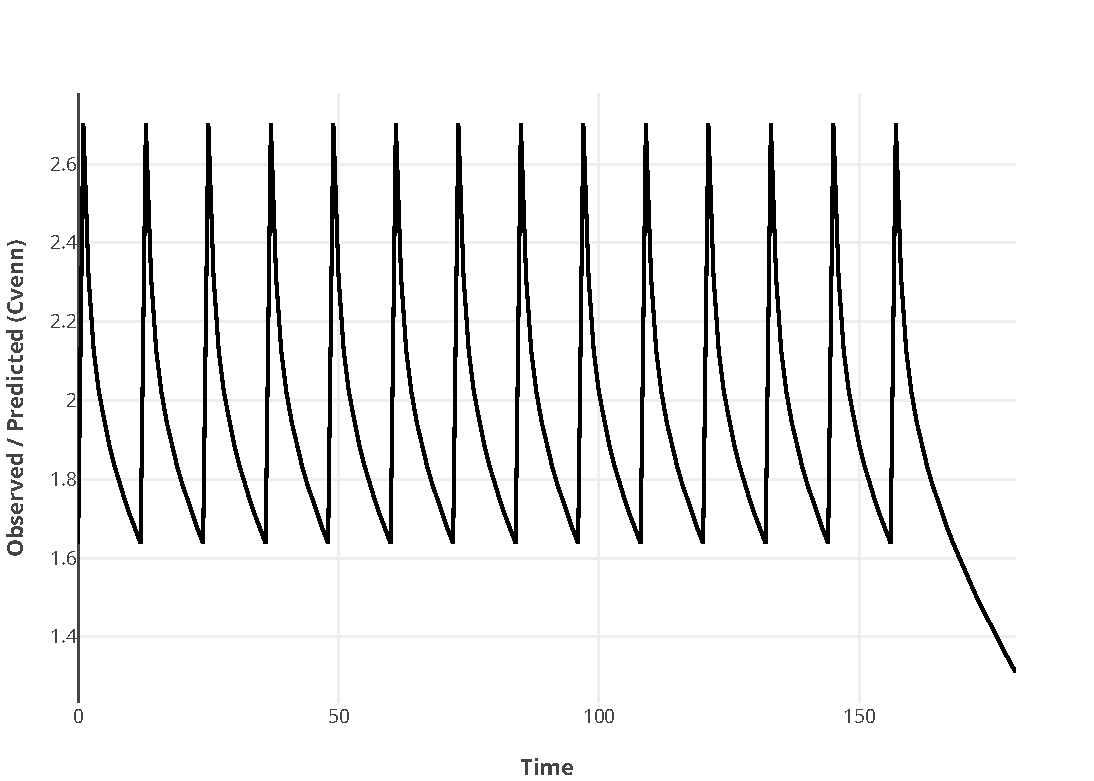
\includegraphics[width=\linewidth]{jl_s6OD6V/vorigsa_6_1.pdf}

We can run parameter estimation on the PBPK model with the \texttt{fit} function, we'll use the simulated data to run the estimation here \texttt{FQad}, \texttt{FQbo}, \texttt{FQbr}, \texttt{FQgu}, \texttt{FQhe}, \texttt{FQki}, \texttt{FQli}, \texttt{FQmu} and \texttt{FQsp} will be estimated within the bounds specified and the other parameters will be fixed.


\begin{lstlisting}
(*@\HLJLn{data}@*) (*@\HLJLoB{=}@*) (*@\HLJLnf{read{\_}pumas}@*)(*@\HLJLp{(}@*)(*@\HLJLnf{DataFrame}@*)(*@\HLJLp{(}@*)(*@\HLJLn{simdata}@*)(*@\HLJLp{),}@*) (*@\HLJLn{observations}@*) (*@\HLJLoB{=}@*) (*@\HLJLp{[}@*)(*@\HLJLsc{:cp}@*)(*@\HLJLp{])}@*)
(*@\HLJLn{ft}@*) (*@\HLJLoB{=}@*) (*@\HLJLnf{fit}@*)(*@\HLJLp{(}@*)(*@\HLJLn{model}@*)(*@\HLJLp{,}@*) (*@\HLJLn{data}@*)(*@\HLJLp{,}@*) (*@\HLJLn{p}@*)(*@\HLJLp{,}@*) (*@\HLJLn{Pumas}@*)(*@\HLJLoB{.}@*)(*@\HLJLnf{NaivePooled}@*)(*@\HLJLp{(),}@*)
    (*@\HLJLn{constantcoef}@*) (*@\HLJLoB{=}@*) (*@\HLJLp{(}@*)
        (*@\HLJLn{Fup}@*) (*@\HLJLoB{=}@*) (*@\HLJLnfB{0.42}@*)(*@\HLJLp{,}@*) (*@\HLJLn{fumic}@*) (*@\HLJLoB{=}@*) (*@\HLJLnfB{0.711}@*)(*@\HLJLp{,}@*) (*@\HLJLn{WEIGHT}@*) (*@\HLJLoB{=}@*) (*@\HLJLni{73}@*)(*@\HLJLp{,}@*) (*@\HLJLn{MPPGL}@*) (*@\HLJLoB{=}@*) (*@\HLJLnfB{30.3}@*)(*@\HLJLp{,}@*) (*@\HLJLn{MPPGI}@*) (*@\HLJLoB{=}@*) (*@\HLJLni{0}@*)(*@\HLJLp{,}@*)
        (*@\HLJLn{C{\_}OUTPUT}@*) (*@\HLJLoB{=}@*) (*@\HLJLnfB{6.5}@*)(*@\HLJLp{,}@*) (*@\HLJLn{VmaxH}@*) (*@\HLJLoB{=}@*) (*@\HLJLni{40}@*)(*@\HLJLp{,}@*) (*@\HLJLn{VmaxG}@*) (*@\HLJLoB{=}@*) (*@\HLJLni{40}@*)(*@\HLJLp{,}@*) (*@\HLJLn{KmH}@*) (*@\HLJLoB{=}@*) (*@\HLJLnfB{9.3}@*)(*@\HLJLp{,}@*) (*@\HLJLn{KmG}@*) (*@\HLJLoB{=}@*) (*@\HLJLnfB{9.3}@*)(*@\HLJLp{,}@*) (*@\HLJLn{bp}@*) (*@\HLJLoB{=}@*) (*@\HLJLni{1}@*)(*@\HLJLp{,}@*)
        (*@\HLJLn{kpad}@*) (*@\HLJLoB{=}@*) (*@\HLJLnfB{9.89}@*)(*@\HLJLp{,}@*) (*@\HLJLn{kpbo}@*) (*@\HLJLoB{=}@*) (*@\HLJLnfB{7.91}@*)(*@\HLJLp{,}@*) (*@\HLJLn{kpbr}@*) (*@\HLJLoB{=}@*) (*@\HLJLnfB{7.35}@*)(*@\HLJLp{,}@*) (*@\HLJLn{kpgu}@*) (*@\HLJLoB{=}@*) (*@\HLJLnfB{5.82}@*)(*@\HLJLp{,}@*) (*@\HLJLn{kphe}@*) (*@\HLJLoB{=}@*) (*@\HLJLnfB{1.95}@*)(*@\HLJLp{,}@*)
        (*@\HLJLn{kpki}@*) (*@\HLJLoB{=}@*) (*@\HLJLnfB{2.9}@*)(*@\HLJLp{,}@*) (*@\HLJLn{kpli}@*) (*@\HLJLoB{=}@*) (*@\HLJLnfB{4.66}@*)(*@\HLJLp{,}@*) (*@\HLJLn{kplu}@*) (*@\HLJLoB{=}@*) (*@\HLJLnfB{0.83}@*)(*@\HLJLp{,}@*) (*@\HLJLn{kpmu}@*) (*@\HLJLoB{=}@*) (*@\HLJLnfB{2.94}@*)(*@\HLJLp{,}@*) (*@\HLJLn{kpsp}@*) (*@\HLJLoB{=}@*) (*@\HLJLnfB{2.96}@*)(*@\HLJLp{,}@*)
        (*@\HLJLn{kpre}@*) (*@\HLJLoB{=}@*) (*@\HLJLni{4}@*)(*@\HLJLp{,}@*) (*@\HLJLn{MW}@*) (*@\HLJLoB{=}@*) (*@\HLJLnfB{349.317}@*)(*@\HLJLp{,}@*) (*@\HLJLn{logP}@*) (*@\HLJLoB{=}@*) (*@\HLJLnfB{2.56}@*)(*@\HLJLp{,}@*) (*@\HLJLn{s{\_}lumen}@*) (*@\HLJLoB{=}@*) (*@\HLJLnfB{0.39}@*)(*@\HLJLoB{*}@*)(*@\HLJLni{1000}@*)(*@\HLJLp{,}@*) (*@\HLJLn{L}@*) (*@\HLJLoB{=}@*) (*@\HLJLni{280}@*)(*@\HLJLp{,}@*)
        (*@\HLJLn{d}@*) (*@\HLJLoB{=}@*) (*@\HLJLnfB{2.5}@*)(*@\HLJLp{,}@*) (*@\HLJLn{PF}@*) (*@\HLJLoB{=}@*) (*@\HLJLnfB{1.57}@*)(*@\HLJLp{,}@*) (*@\HLJLn{VF}@*) (*@\HLJLoB{=}@*) (*@\HLJLnfB{6.5}@*)(*@\HLJLp{,}@*) (*@\HLJLn{MF}@*) (*@\HLJLoB{=}@*) (*@\HLJLni{13}@*)(*@\HLJLp{,}@*) (*@\HLJLn{ITT}@*) (*@\HLJLoB{=}@*) (*@\HLJLnfB{3.32}@*)(*@\HLJLp{,}@*) (*@\HLJLn{A}@*) (*@\HLJLoB{=}@*) (*@\HLJLni{7440}@*)(*@\HLJLp{,}@*) (*@\HLJLn{B}@*) (*@\HLJLoB{=}@*) (*@\HLJLnfB{1e7}@*)(*@\HLJLp{,}@*)
        (*@\HLJLn{alpha}@*) (*@\HLJLoB{=}@*) (*@\HLJLnfB{0.6}@*)(*@\HLJLp{,}@*) (*@\HLJLn{beta}@*) (*@\HLJLoB{=}@*) (*@\HLJLnfB{4.395}@*)(*@\HLJLp{,}@*) (*@\HLJLn{fabs}@*) (*@\HLJLoB{=}@*) (*@\HLJLni{1}@*)(*@\HLJLp{,}@*) (*@\HLJLn{fdis}@*) (*@\HLJLoB{=}@*) (*@\HLJLni{1}@*)(*@\HLJLp{,}@*) (*@\HLJLn{fperm}@*) (*@\HLJLoB{=}@*) (*@\HLJLni{1}@*)(*@\HLJLp{,}@*) (*@\HLJLn{vad}@*) (*@\HLJLoB{=}@*) (*@\HLJLnfB{18.2}@*)(*@\HLJLp{,}@*)
        (*@\HLJLn{vbo}@*) (*@\HLJLoB{=}@*) (*@\HLJLnfB{10.5}@*)(*@\HLJLp{,}@*) (*@\HLJLn{vbr}@*) (*@\HLJLoB{=}@*) (*@\HLJLnfB{1.45}@*)(*@\HLJLp{,}@*) (*@\HLJLn{vguWall}@*) (*@\HLJLoB{=}@*) (*@\HLJLnfB{0.65}@*)(*@\HLJLp{,}@*) (*@\HLJLn{vgulumen}@*) (*@\HLJLoB{=}@*) (*@\HLJLnfB{0.35}@*)(*@\HLJLp{,}@*) (*@\HLJLn{vhe}@*) (*@\HLJLoB{=}@*) (*@\HLJLnfB{0.33}@*)(*@\HLJLp{,}@*)
        (*@\HLJLn{vki}@*) (*@\HLJLoB{=}@*) (*@\HLJLnfB{0.31}@*)(*@\HLJLp{,}@*) (*@\HLJLn{vli}@*) (*@\HLJLoB{=}@*) (*@\HLJLnfB{1.8}@*)(*@\HLJLp{,}@*) (*@\HLJLn{vlu}@*) (*@\HLJLoB{=}@*) (*@\HLJLnfB{0.5}@*)(*@\HLJLp{,}@*) (*@\HLJLn{vmu}@*) (*@\HLJLoB{=}@*) (*@\HLJLni{29}@*)(*@\HLJLp{,}@*) (*@\HLJLn{vsp}@*) (*@\HLJLoB{=}@*) (*@\HLJLnfB{0.15}@*)(*@\HLJLp{,}@*) (*@\HLJLn{vbl}@*) (*@\HLJLoB{=}@*) (*@\HLJLnfB{5.6}@*)(*@\HLJLp{),}@*)
    (*@\HLJLn{ensemblealg}@*)(*@\HLJLoB{=}@*)(*@\HLJLnf{EnsembleThreads}@*)(*@\HLJLp{())}@*)
\end{lstlisting}

\begin{lstlisting}
Iter     Function value   Gradient norm 
     0     3.682016e+03     2.752213e+02
 * time: 6.198883056640625e-5
     1     3.252025e+03     4.512975e+02
 * time: 0.4183320999145508
     2     2.343474e+03     5.140776e+02
 * time: 0.7970240116119385
     3     1.766600e+03     1.200491e+02
 * time: 1.1807188987731934
     4     1.695758e+03     6.517564e+01
 * time: 1.5688560009002686
     5     1.571057e+03     1.089599e+02
 * time: 1.9491629600524902
     6     1.388413e+03     1.741696e+02
 * time: 2.4055609703063965
     7     1.334351e+03     3.132303e+02
 * time: 2.8494529724121094
     8     1.206765e+03     8.085562e+02
 * time: 3.2726891040802
     9     1.028465e+03     9.440923e+01
 * time: 3.7250359058380127
    10     1.011599e+03     3.657840e+01
 * time: 4.110250949859619
    11     1.005571e+03     2.707605e+01
 * time: 4.4939069747924805
    12     9.968068e+02     7.390553e+00
 * time: 4.883265972137451
    13     9.955940e+02     4.583467e+00
 * time: 5.368079900741577
    14     9.950436e+02     1.395316e+01
 * time: 5.80047607421875
    15     9.944541e+02     2.221676e+01
 * time: 6.185312986373901
    16     9.933581e+02     2.684005e+01
 * time: 6.572652101516724
    17     9.925532e+02     1.810444e+01
 * time: 7.623115062713623
    18     9.923363e+02     1.217759e+01
 * time: 8.003284931182861
    19     9.921507e+02     7.880794e+00
 * time: 8.384046077728271
    20     9.919460e+02     3.910831e+00
 * time: 8.763987064361572
    21     9.918746e+02     1.856312e+00
 * time: 9.145912885665894
    22     9.918594e+02     5.778782e-01
 * time: 9.52832293510437
    23     9.918563e+02     6.030107e-01
 * time: 9.911438941955566
    24     9.918552e+02     6.843451e-01
 * time: 10.29286003112793
    25     9.918543e+02     6.338827e-01
 * time: 10.676716089248657
    26     9.918533e+02     7.920941e-01
 * time: 11.060359954833984
    27     9.918514e+02     9.417454e-01
 * time: 11.444878101348877
    28     9.918472e+02     1.073079e+00
 * time: 11.827600955963135
    29     9.918381e+02     1.113643e+00
 * time: 12.211363077163696
    30     9.918214e+02     9.769528e-01
 * time: 12.59877896308899
    31     9.917985e+02     1.080627e+00
 * time: 12.9826180934906
    32     9.917786e+02     8.564848e-01
 * time: 13.366760015487671
    33     9.917363e+02     1.767720e+00
 * time: 13.751688003540039
    34     9.916116e+02     5.550372e+00
 * time: 14.134628057479858
    35     9.914442e+02     1.629176e+01
 * time: 14.518476009368896
    36     9.912107e+02     1.914126e+01
 * time: 14.902476072311401
    37     9.909221e+02     1.818566e+00
 * time: 15.29062795639038
    38     9.907569e+02     1.334672e+00
 * time: 15.673218011856079
    39     9.891721e+02     3.625843e+00
 * time: 16.057929039001465
    40     9.873604e+02     8.709680e+00
 * time: 16.510833024978638
    41     9.853998e+02     1.721744e+01
 * time: 16.966166973114014
    42     9.827862e+02     3.346704e+01
 * time: 17.48515510559082
    43     9.808133e+02     3.868350e+01
 * time: 17.8686580657959
    44     9.799189e+02     1.230831e+01
 * time: 18.256328105926514
    45     9.789635e+02     8.525065e+00
 * time: 18.645689010620117
    46     9.787814e+02     1.170915e+00
 * time: 19.031748056411743
    47     9.787113e+02     8.322856e-01
 * time: 19.957097053527832
    48     9.786777e+02     1.542617e+00
 * time: 20.339303970336914
    49     9.786629e+02     1.973609e+00
 * time: 20.72168803215027
    50     9.786532e+02     2.149714e+00
 * time: 21.106795072555542
    51     9.786342e+02     2.332614e+00
 * time: 21.48783302307129
    52     9.785897e+02     2.740712e+00
 * time: 21.869559049606323
    53     9.784831e+02     3.213833e+00
 * time: 22.249927043914795
    54     9.782695e+02     3.918206e+00
 * time: 22.63142991065979
    55     9.781810e+02     1.392242e+01
 * time: 23.01122498512268
    56     9.780437e+02     3.907756e+00
 * time: 23.389700889587402
    57     9.779749e+02     3.637655e+00
 * time: 23.768632888793945
    58     9.779138e+02     5.239207e+00
 * time: 24.150371074676514
    59     9.778386e+02     4.021796e+00
 * time: 24.532577991485596
    60     9.777753e+02     1.528757e+00
 * time: 24.917359113693237
    61     9.777552e+02     4.086616e+00
 * time: 25.368921995162964
    62     9.777179e+02     1.984431e+00
 * time: 25.755944967269897
    63     9.777034e+02     1.097987e+00
 * time: 26.14190101623535
    64     9.776927e+02     2.070626e+00
 * time: 26.5276460647583
    65     9.776884e+02     1.606587e-01
 * time: 27.04797101020813
    66     9.776875e+02     2.689506e-01
 * time: 27.426809072494507
    67     9.776872e+02     1.312477e-01
 * time: 27.804589986801147
    68     9.776872e+02     9.005929e-03
 * time: 28.18191695213318
    69     9.776872e+02     9.003301e-03
 * time: 28.822920083999634
    70     9.776872e+02     9.003301e-03
 * time: 29.74469494819641
FittedPumasModel

Successful minimization:                      true

Likelihood approximation:        Pumas.NaivePooled
Log-likelihood value:                   -977.68717
Number of subjects:                              1
Number of parameters:         Fixed      Optimized
                                 50              9
Observation records:         Active        Missing
    cp:                         181              0
    Total:                      181              0

-------------------------
             Estimate
-------------------------
Fup           0.42
fumic         0.711
WEIGHT       73.0
MPPGL        30.3
MPPGI         0.0
C(*@{{\_}}@*)OUTPUT      6.5
VmaxH        40.0
VmaxG        40.0
KmH           9.3
KmG           9.3
bp            1.0
kpad          9.89
kpbo          7.91
kpbr          7.35
kpgu          5.82
kphe          1.95
kpki          2.9
kpli          4.66
kplu          0.83
kpmu          2.94
kpsp          2.96
kpre          4.0
MW          349.32
logP          2.56
s(*@{{\_}}@*)lumen     390.0
L           280.0
d             2.5
PF            1.57
VF            6.5
MF           13.0
ITT           3.32
A          7440.0
B             1.0e7
alpha         0.6
beta          4.395
fabs          1.0
fdis          1.0
fperm         1.0
vad          18.2
vbo          10.5
vbr           1.45
vguWall       0.65
vgulumen      0.35
vhe           0.33
vki           0.31
vli           1.8
vlu           0.5
vmu          29.0
vsp           0.15
vbl           5.6
FQad          6.0121e-98
FQbo          3.6745e-82
FQbr          0.032632
FQgu          0.030202
FQhe          0.023345
FQki          1.7398e-11
FQli          0.62779
FQmu          0.26102
FQsp          0.97984
-------------------------
\end{lstlisting}


\subsubsection{GSA}
We'll run the GSA on the AUC and Cmax output of the \texttt{Cvenn} variable and therefore redefine the model to include the NCA calculation.


\begin{lstlisting}
(*@\HLJLn{model}@*) (*@\HLJLoB{=}@*) (*@\HLJLnd{@model}@*) (*@\HLJLk{begin}@*)
    (*@\HLJLnd{@param}@*) (*@\HLJLk{begin}@*)
        (*@\HLJLn{Fup}@*) (*@\HLJLoB{\ensuremath{\in}}@*) (*@\HLJLnf{RealDomain}@*)(*@\HLJLp{(}@*)(*@\HLJLn{init}@*) (*@\HLJLoB{=}@*) (*@\HLJLnfB{0.42}@*)(*@\HLJLp{)}@*)
        (*@\HLJLn{fumic}@*) (*@\HLJLoB{\ensuremath{\in}}@*) (*@\HLJLnf{RealDomain}@*)(*@\HLJLp{(}@*)(*@\HLJLn{init}@*) (*@\HLJLoB{=}@*) (*@\HLJLnfB{0.711}@*)(*@\HLJLp{)}@*)
        (*@\HLJLn{WEIGHT}@*) (*@\HLJLoB{\ensuremath{\in}}@*) (*@\HLJLnf{RealDomain}@*)(*@\HLJLp{(}@*)(*@\HLJLn{init}@*) (*@\HLJLoB{=}@*) (*@\HLJLni{73}@*)(*@\HLJLp{)}@*)
        (*@\HLJLn{MPPGL}@*) (*@\HLJLoB{\ensuremath{\in}}@*) (*@\HLJLnf{RealDomain}@*)(*@\HLJLp{(}@*)(*@\HLJLn{init}@*) (*@\HLJLoB{=}@*) (*@\HLJLnfB{30.3}@*)(*@\HLJLp{)}@*)
        (*@\HLJLn{MPPGI}@*) (*@\HLJLoB{\ensuremath{\in}}@*) (*@\HLJLnf{RealDomain}@*)(*@\HLJLp{(}@*)(*@\HLJLn{init}@*) (*@\HLJLoB{=}@*) (*@\HLJLni{0}@*)(*@\HLJLp{)}@*)
        (*@\HLJLn{C{\_}OUTPUT}@*) (*@\HLJLoB{\ensuremath{\in}}@*) (*@\HLJLnf{RealDomain}@*)(*@\HLJLp{(}@*)(*@\HLJLn{init}@*) (*@\HLJLoB{=}@*) (*@\HLJLnfB{6.5}@*)(*@\HLJLp{)}@*)
        (*@\HLJLn{VmaxH}@*) (*@\HLJLoB{\ensuremath{\in}}@*) (*@\HLJLnf{RealDomain}@*)(*@\HLJLp{(}@*)(*@\HLJLn{init}@*) (*@\HLJLoB{=}@*) (*@\HLJLni{40}@*)(*@\HLJLp{)}@*)
        (*@\HLJLn{VmaxG}@*) (*@\HLJLoB{\ensuremath{\in}}@*) (*@\HLJLnf{RealDomain}@*)(*@\HLJLp{(}@*)(*@\HLJLn{init}@*) (*@\HLJLoB{=}@*) (*@\HLJLni{40}@*)(*@\HLJLp{)}@*)
        (*@\HLJLn{KmH}@*) (*@\HLJLoB{\ensuremath{\in}}@*) (*@\HLJLnf{RealDomain}@*)(*@\HLJLp{(}@*)(*@\HLJLn{init}@*) (*@\HLJLoB{=}@*) (*@\HLJLnfB{9.3}@*)(*@\HLJLp{)}@*)
        (*@\HLJLn{KmG}@*) (*@\HLJLoB{\ensuremath{\in}}@*) (*@\HLJLnf{RealDomain}@*)(*@\HLJLp{(}@*)(*@\HLJLn{init}@*) (*@\HLJLoB{=}@*) (*@\HLJLnfB{9.3}@*)(*@\HLJLp{)}@*)
        (*@\HLJLn{bp}@*) (*@\HLJLoB{\ensuremath{\in}}@*) (*@\HLJLnf{RealDomain}@*)(*@\HLJLp{(}@*)(*@\HLJLn{init}@*) (*@\HLJLoB{=}@*) (*@\HLJLni{1}@*)(*@\HLJLp{)}@*)
        (*@\HLJLn{kpad}@*) (*@\HLJLoB{\ensuremath{\in}}@*) (*@\HLJLnf{RealDomain}@*)(*@\HLJLp{(}@*)(*@\HLJLn{init}@*) (*@\HLJLoB{=}@*) (*@\HLJLnfB{9.89}@*)(*@\HLJLp{)}@*)
        (*@\HLJLn{kpbo}@*) (*@\HLJLoB{\ensuremath{\in}}@*) (*@\HLJLnf{RealDomain}@*)(*@\HLJLp{(}@*)(*@\HLJLn{init}@*) (*@\HLJLoB{=}@*) (*@\HLJLnfB{7.91}@*)(*@\HLJLp{)}@*)
        (*@\HLJLn{kpbr}@*) (*@\HLJLoB{\ensuremath{\in}}@*) (*@\HLJLnf{RealDomain}@*)(*@\HLJLp{(}@*)(*@\HLJLn{init}@*) (*@\HLJLoB{=}@*) (*@\HLJLnfB{7.35}@*)(*@\HLJLp{)}@*)
        (*@\HLJLn{kpgu}@*) (*@\HLJLoB{\ensuremath{\in}}@*) (*@\HLJLnf{RealDomain}@*)(*@\HLJLp{(}@*)(*@\HLJLn{init}@*) (*@\HLJLoB{=}@*) (*@\HLJLnfB{5.82}@*)(*@\HLJLp{)}@*)
        (*@\HLJLn{kphe}@*) (*@\HLJLoB{\ensuremath{\in}}@*) (*@\HLJLnf{RealDomain}@*)(*@\HLJLp{(}@*)(*@\HLJLn{init}@*) (*@\HLJLoB{=}@*) (*@\HLJLnfB{1.95}@*)(*@\HLJLp{)}@*)
        (*@\HLJLn{kpki}@*) (*@\HLJLoB{\ensuremath{\in}}@*) (*@\HLJLnf{RealDomain}@*)(*@\HLJLp{(}@*)(*@\HLJLn{init}@*) (*@\HLJLoB{=}@*) (*@\HLJLnfB{2.9}@*)(*@\HLJLp{)}@*)
        (*@\HLJLn{kpli}@*) (*@\HLJLoB{\ensuremath{\in}}@*) (*@\HLJLnf{RealDomain}@*)(*@\HLJLp{(}@*)(*@\HLJLn{init}@*) (*@\HLJLoB{=}@*) (*@\HLJLnfB{4.66}@*)(*@\HLJLp{)}@*)
        (*@\HLJLn{kplu}@*) (*@\HLJLoB{\ensuremath{\in}}@*) (*@\HLJLnf{RealDomain}@*)(*@\HLJLp{(}@*)(*@\HLJLn{init}@*) (*@\HLJLoB{=}@*) (*@\HLJLnfB{0.83}@*)(*@\HLJLp{)}@*)
        (*@\HLJLn{kpmu}@*) (*@\HLJLoB{\ensuremath{\in}}@*) (*@\HLJLnf{RealDomain}@*)(*@\HLJLp{(}@*)(*@\HLJLn{init}@*) (*@\HLJLoB{=}@*) (*@\HLJLnfB{2.94}@*)(*@\HLJLp{)}@*)
        (*@\HLJLn{kpsp}@*) (*@\HLJLoB{\ensuremath{\in}}@*) (*@\HLJLnf{RealDomain}@*)(*@\HLJLp{(}@*)(*@\HLJLn{init}@*) (*@\HLJLoB{=}@*) (*@\HLJLnfB{2.96}@*)(*@\HLJLp{)}@*)
        (*@\HLJLn{kpre}@*) (*@\HLJLoB{\ensuremath{\in}}@*) (*@\HLJLnf{RealDomain}@*)(*@\HLJLp{(}@*)(*@\HLJLn{init}@*) (*@\HLJLoB{=}@*) (*@\HLJLni{4}@*)(*@\HLJLp{)}@*)
        (*@\HLJLn{MW}@*) (*@\HLJLoB{\ensuremath{\in}}@*) (*@\HLJLnf{RealDomain}@*)(*@\HLJLp{(}@*)(*@\HLJLn{init}@*) (*@\HLJLoB{=}@*) (*@\HLJLnfB{349.317}@*)(*@\HLJLp{)}@*)
        (*@\HLJLn{logP}@*) (*@\HLJLoB{\ensuremath{\in}}@*) (*@\HLJLnf{RealDomain}@*)(*@\HLJLp{(}@*)(*@\HLJLn{init}@*) (*@\HLJLoB{=}@*) (*@\HLJLnfB{2.56}@*)(*@\HLJLp{)}@*)
        (*@\HLJLn{s{\_}lumen}@*) (*@\HLJLoB{\ensuremath{\in}}@*) (*@\HLJLnf{RealDomain}@*)(*@\HLJLp{(}@*)(*@\HLJLn{init}@*) (*@\HLJLoB{=}@*) (*@\HLJLnfB{0.39}@*)(*@\HLJLoB{*}@*)(*@\HLJLni{1000}@*)(*@\HLJLp{)}@*)
        (*@\HLJLn{L}@*) (*@\HLJLoB{\ensuremath{\in}}@*) (*@\HLJLnf{RealDomain}@*)(*@\HLJLp{(}@*)(*@\HLJLn{init}@*) (*@\HLJLoB{=}@*) (*@\HLJLni{280}@*)(*@\HLJLp{)}@*)
        (*@\HLJLn{d}@*) (*@\HLJLoB{\ensuremath{\in}}@*) (*@\HLJLnf{RealDomain}@*)(*@\HLJLp{(}@*)(*@\HLJLn{init}@*) (*@\HLJLoB{=}@*) (*@\HLJLnfB{2.5}@*)(*@\HLJLp{)}@*)
        (*@\HLJLn{PF}@*) (*@\HLJLoB{\ensuremath{\in}}@*) (*@\HLJLnf{RealDomain}@*)(*@\HLJLp{(}@*)(*@\HLJLn{init}@*) (*@\HLJLoB{=}@*) (*@\HLJLnfB{1.57}@*)(*@\HLJLp{)}@*)
        (*@\HLJLn{VF}@*) (*@\HLJLoB{\ensuremath{\in}}@*) (*@\HLJLnf{RealDomain}@*)(*@\HLJLp{(}@*)(*@\HLJLn{init}@*) (*@\HLJLoB{=}@*) (*@\HLJLnfB{6.5}@*)(*@\HLJLp{)}@*)
        (*@\HLJLn{MF}@*) (*@\HLJLoB{\ensuremath{\in}}@*) (*@\HLJLnf{RealDomain}@*)(*@\HLJLp{(}@*)(*@\HLJLn{init}@*) (*@\HLJLoB{=}@*) (*@\HLJLni{13}@*)(*@\HLJLp{)}@*)
        (*@\HLJLn{ITT}@*) (*@\HLJLoB{\ensuremath{\in}}@*) (*@\HLJLnf{RealDomain}@*)(*@\HLJLp{(}@*)(*@\HLJLn{init}@*) (*@\HLJLoB{=}@*) (*@\HLJLnfB{3.32}@*)(*@\HLJLp{)}@*)
        (*@\HLJLn{A}@*) (*@\HLJLoB{\ensuremath{\in}}@*) (*@\HLJLnf{RealDomain}@*)(*@\HLJLp{(}@*)(*@\HLJLn{init}@*) (*@\HLJLoB{=}@*) (*@\HLJLni{7440}@*)(*@\HLJLp{)}@*)
        (*@\HLJLn{B}@*) (*@\HLJLoB{\ensuremath{\in}}@*) (*@\HLJLnf{RealDomain}@*)(*@\HLJLp{(}@*)(*@\HLJLn{init}@*) (*@\HLJLoB{=}@*) (*@\HLJLnfB{1e7}@*)(*@\HLJLp{)}@*)
        (*@\HLJLn{alpha}@*) (*@\HLJLoB{\ensuremath{\in}}@*) (*@\HLJLnf{RealDomain}@*)(*@\HLJLp{(}@*)(*@\HLJLn{init}@*) (*@\HLJLoB{=}@*) (*@\HLJLnfB{0.6}@*)(*@\HLJLp{)}@*)
        (*@\HLJLn{beta}@*) (*@\HLJLoB{\ensuremath{\in}}@*) (*@\HLJLnf{RealDomain}@*)(*@\HLJLp{(}@*)(*@\HLJLn{init}@*) (*@\HLJLoB{=}@*) (*@\HLJLnfB{4.395}@*)(*@\HLJLp{)}@*)
        (*@\HLJLn{fabs}@*) (*@\HLJLoB{\ensuremath{\in}}@*) (*@\HLJLnf{RealDomain}@*)(*@\HLJLp{(}@*)(*@\HLJLn{init}@*) (*@\HLJLoB{=}@*) (*@\HLJLni{1}@*)(*@\HLJLp{)}@*)
        (*@\HLJLn{fdis}@*) (*@\HLJLoB{\ensuremath{\in}}@*) (*@\HLJLnf{RealDomain}@*)(*@\HLJLp{(}@*)(*@\HLJLn{init}@*) (*@\HLJLoB{=}@*) (*@\HLJLni{1}@*)(*@\HLJLp{)}@*)
        (*@\HLJLn{fperm}@*) (*@\HLJLoB{\ensuremath{\in}}@*) (*@\HLJLnf{RealDomain}@*)(*@\HLJLp{(}@*)(*@\HLJLn{init}@*) (*@\HLJLoB{=}@*) (*@\HLJLni{1}@*)(*@\HLJLp{)}@*)
        (*@\HLJLn{vad}@*) (*@\HLJLoB{\ensuremath{\in}}@*) (*@\HLJLnf{RealDomain}@*)(*@\HLJLp{(}@*)(*@\HLJLn{init}@*) (*@\HLJLoB{=}@*) (*@\HLJLnfB{18.2}@*)(*@\HLJLp{)}@*)
        (*@\HLJLn{vbo}@*) (*@\HLJLoB{\ensuremath{\in}}@*) (*@\HLJLnf{RealDomain}@*)(*@\HLJLp{(}@*)(*@\HLJLn{init}@*) (*@\HLJLoB{=}@*)(*@\HLJLnfB{10.5}@*)(*@\HLJLp{)}@*)
        (*@\HLJLn{vbr}@*) (*@\HLJLoB{\ensuremath{\in}}@*) (*@\HLJLnf{RealDomain}@*)(*@\HLJLp{(}@*)(*@\HLJLn{init}@*) (*@\HLJLoB{=}@*)(*@\HLJLnfB{1.45}@*)(*@\HLJLp{)}@*)
        (*@\HLJLn{vguWall}@*) (*@\HLJLoB{\ensuremath{\in}}@*) (*@\HLJLnf{RealDomain}@*)(*@\HLJLp{(}@*)(*@\HLJLn{init}@*) (*@\HLJLoB{=}@*)(*@\HLJLnfB{0.65}@*)(*@\HLJLp{)}@*)
        (*@\HLJLn{vgulumen}@*) (*@\HLJLoB{\ensuremath{\in}}@*) (*@\HLJLnf{RealDomain}@*)(*@\HLJLp{(}@*)(*@\HLJLn{init}@*) (*@\HLJLoB{=}@*)(*@\HLJLnfB{0.35}@*)(*@\HLJLp{)}@*)
        (*@\HLJLn{vhe}@*) (*@\HLJLoB{\ensuremath{\in}}@*) (*@\HLJLnf{RealDomain}@*)(*@\HLJLp{(}@*)(*@\HLJLn{init}@*) (*@\HLJLoB{=}@*)(*@\HLJLnfB{0.33}@*)(*@\HLJLp{)}@*)
        (*@\HLJLn{vki}@*) (*@\HLJLoB{\ensuremath{\in}}@*) (*@\HLJLnf{RealDomain}@*)(*@\HLJLp{(}@*)(*@\HLJLn{init}@*) (*@\HLJLoB{=}@*)(*@\HLJLnfB{0.31}@*)(*@\HLJLp{)}@*)
        (*@\HLJLn{vli}@*) (*@\HLJLoB{\ensuremath{\in}}@*) (*@\HLJLnf{RealDomain}@*)(*@\HLJLp{(}@*)(*@\HLJLn{init}@*) (*@\HLJLoB{=}@*)(*@\HLJLnfB{1.8}@*)(*@\HLJLp{)}@*)
        (*@\HLJLn{vlu}@*) (*@\HLJLoB{\ensuremath{\in}}@*) (*@\HLJLnf{RealDomain}@*)(*@\HLJLp{(}@*)(*@\HLJLn{init}@*) (*@\HLJLoB{=}@*)(*@\HLJLnfB{0.5}@*)(*@\HLJLp{)}@*)
        (*@\HLJLn{vmu}@*) (*@\HLJLoB{\ensuremath{\in}}@*) (*@\HLJLnf{RealDomain}@*)(*@\HLJLp{(}@*)(*@\HLJLn{init}@*) (*@\HLJLoB{=}@*)(*@\HLJLni{29}@*)(*@\HLJLp{)}@*)
        (*@\HLJLn{vsp}@*) (*@\HLJLoB{\ensuremath{\in}}@*) (*@\HLJLnf{RealDomain}@*)(*@\HLJLp{(}@*)(*@\HLJLn{init}@*) (*@\HLJLoB{=}@*)(*@\HLJLnfB{0.15}@*)(*@\HLJLp{)}@*)
        (*@\HLJLn{vbl}@*) (*@\HLJLoB{\ensuremath{\in}}@*) (*@\HLJLnf{RealDomain}@*)(*@\HLJLp{(}@*)(*@\HLJLn{init}@*) (*@\HLJLoB{=}@*)(*@\HLJLnfB{5.6}@*)(*@\HLJLp{)}@*)
        (*@\HLJLn{FQad}@*) (*@\HLJLoB{\ensuremath{\in}}@*) (*@\HLJLnf{RealDomain}@*)(*@\HLJLp{(}@*)(*@\HLJLn{lower}@*) (*@\HLJLoB{=}@*) (*@\HLJLnfB{0.0}@*)(*@\HLJLp{,}@*) (*@\HLJLn{init}@*) (*@\HLJLoB{=}@*) (*@\HLJLnfB{0.05}@*)(*@\HLJLp{,}@*) (*@\HLJLn{upper}@*) (*@\HLJLoB{=}@*) (*@\HLJLnfB{1.0}@*)(*@\HLJLp{)}@*)
        (*@\HLJLn{FQbo}@*) (*@\HLJLoB{\ensuremath{\in}}@*) (*@\HLJLnf{RealDomain}@*)(*@\HLJLp{(}@*)(*@\HLJLn{lower}@*) (*@\HLJLoB{=}@*) (*@\HLJLnfB{0.0}@*)(*@\HLJLp{,}@*) (*@\HLJLn{init}@*) (*@\HLJLoB{=}@*) (*@\HLJLnfB{0.05}@*)(*@\HLJLp{,}@*) (*@\HLJLn{upper}@*) (*@\HLJLoB{=}@*) (*@\HLJLnfB{1.0}@*)(*@\HLJLp{)}@*)
        (*@\HLJLn{FQbr}@*) (*@\HLJLoB{\ensuremath{\in}}@*) (*@\HLJLnf{RealDomain}@*)(*@\HLJLp{(}@*)(*@\HLJLn{lower}@*) (*@\HLJLoB{=}@*) (*@\HLJLnfB{0.0}@*)(*@\HLJLp{,}@*) (*@\HLJLn{init}@*) (*@\HLJLoB{=}@*) (*@\HLJLnfB{0.12}@*)(*@\HLJLp{,}@*) (*@\HLJLn{upper}@*) (*@\HLJLoB{=}@*) (*@\HLJLnfB{1.0}@*)(*@\HLJLp{)}@*)
        (*@\HLJLn{FQgu}@*) (*@\HLJLoB{\ensuremath{\in}}@*) (*@\HLJLnf{RealDomain}@*)(*@\HLJLp{(}@*)(*@\HLJLn{lower}@*) (*@\HLJLoB{=}@*) (*@\HLJLnfB{0.0}@*)(*@\HLJLp{,}@*) (*@\HLJLn{init}@*) (*@\HLJLoB{=}@*) (*@\HLJLnfB{0.16}@*)(*@\HLJLp{,}@*) (*@\HLJLn{upper}@*) (*@\HLJLoB{=}@*) (*@\HLJLnfB{1.0}@*)(*@\HLJLp{)}@*)
        (*@\HLJLn{FQhe}@*) (*@\HLJLoB{\ensuremath{\in}}@*) (*@\HLJLnf{RealDomain}@*)(*@\HLJLp{(}@*)(*@\HLJLn{lower}@*) (*@\HLJLoB{=}@*) (*@\HLJLnfB{0.0}@*)(*@\HLJLp{,}@*) (*@\HLJLn{init}@*) (*@\HLJLoB{=}@*) (*@\HLJLnfB{0.04}@*)(*@\HLJLp{,}@*) (*@\HLJLn{upper}@*) (*@\HLJLoB{=}@*) (*@\HLJLnfB{1.0}@*)(*@\HLJLp{)}@*)
        (*@\HLJLn{FQki}@*) (*@\HLJLoB{\ensuremath{\in}}@*) (*@\HLJLnf{RealDomain}@*)(*@\HLJLp{(}@*)(*@\HLJLn{lower}@*) (*@\HLJLoB{=}@*) (*@\HLJLnfB{0.0}@*)(*@\HLJLp{,}@*) (*@\HLJLn{init}@*) (*@\HLJLoB{=}@*) (*@\HLJLnfB{0.19}@*)(*@\HLJLp{,}@*) (*@\HLJLn{upper}@*) (*@\HLJLoB{=}@*) (*@\HLJLnfB{1.0}@*)(*@\HLJLp{)}@*)
        (*@\HLJLn{FQli}@*) (*@\HLJLoB{\ensuremath{\in}}@*) (*@\HLJLnf{RealDomain}@*)(*@\HLJLp{(}@*)(*@\HLJLn{lower}@*) (*@\HLJLoB{=}@*) (*@\HLJLnfB{0.0}@*)(*@\HLJLp{,}@*) (*@\HLJLn{init}@*) (*@\HLJLoB{=}@*) (*@\HLJLnfB{0.255}@*)(*@\HLJLp{,}@*) (*@\HLJLn{upper}@*) (*@\HLJLoB{=}@*) (*@\HLJLnfB{1.0}@*)(*@\HLJLp{)}@*)
        (*@\HLJLn{FQmu}@*) (*@\HLJLoB{\ensuremath{\in}}@*) (*@\HLJLnf{RealDomain}@*)(*@\HLJLp{(}@*)(*@\HLJLn{lower}@*) (*@\HLJLoB{=}@*) (*@\HLJLnfB{0.0}@*)(*@\HLJLp{,}@*) (*@\HLJLn{init}@*) (*@\HLJLoB{=}@*) (*@\HLJLnfB{0.17}@*)(*@\HLJLp{,}@*) (*@\HLJLn{upper}@*) (*@\HLJLoB{=}@*) (*@\HLJLnfB{1.0}@*)(*@\HLJLp{)}@*)
        (*@\HLJLn{FQsp}@*) (*@\HLJLoB{\ensuremath{\in}}@*) (*@\HLJLnf{RealDomain}@*)(*@\HLJLp{(}@*)(*@\HLJLn{lower}@*) (*@\HLJLoB{=}@*) (*@\HLJLnfB{0.0}@*)(*@\HLJLp{,}@*) (*@\HLJLn{init}@*) (*@\HLJLoB{=}@*) (*@\HLJLnfB{0.03}@*)(*@\HLJLp{,}@*) (*@\HLJLn{upper}@*) (*@\HLJLoB{=}@*) (*@\HLJLnfB{1.0}@*)(*@\HLJLp{)}@*)
    (*@\HLJLk{end}@*)
    (*@\HLJLnd{@pre}@*) (*@\HLJLk{begin}@*)
        (*@\HLJLn{Vgu}@*) (*@\HLJLoB{=}@*) (*@\HLJLn{vguWall}@*) (*@\HLJLoB{+}@*) (*@\HLJLn{vgulumen}@*)
        (*@\HLJLn{Vve}@*) (*@\HLJLoB{=}@*) (*@\HLJLnfB{0.705}@*)(*@\HLJLoB{*}@*)(*@\HLJLn{vbl}@*)
        (*@\HLJLn{Var}@*) (*@\HLJLoB{=}@*) (*@\HLJLnfB{0.295}@*)(*@\HLJLoB{*}@*)(*@\HLJLn{vbl}@*)
        (*@\HLJLn{Vre}@*) (*@\HLJLoB{=}@*) (*@\HLJLn{WEIGHT}@*) (*@\HLJLoB{-}@*) (*@\HLJLp{(}@*)(*@\HLJLn{vli}@*)(*@\HLJLoB{+}@*)(*@\HLJLn{vki}@*)(*@\HLJLoB{+}@*)(*@\HLJLn{vsp}@*)(*@\HLJLoB{+}@*)(*@\HLJLn{vhe}@*)(*@\HLJLoB{+}@*)(*@\HLJLn{vlu}@*)(*@\HLJLoB{+}@*)(*@\HLJLn{vbo}@*)(*@\HLJLoB{+}@*)(*@\HLJLn{vbr}@*)(*@\HLJLoB{+}@*)(*@\HLJLn{vmu}@*)(*@\HLJLoB{+}@*)(*@\HLJLn{vad}@*)(*@\HLJLoB{+}@*)(*@\HLJLn{vguWall}@*)(*@\HLJLoB{+}@*)(*@\HLJLn{vbl}@*)(*@\HLJLp{)}@*)
        (*@\HLJLn{CO}@*) (*@\HLJLoB{=}@*) (*@\HLJLn{C{\_}OUTPUT}@*)(*@\HLJLoB{*}@*)(*@\HLJLni{60}@*)
        (*@\HLJLn{Qad}@*) (*@\HLJLoB{=}@*) (*@\HLJLn{FQad}@*)(*@\HLJLoB{*}@*)(*@\HLJLn{CO}@*)
        (*@\HLJLn{Qbo}@*) (*@\HLJLoB{=}@*) (*@\HLJLn{FQbo}@*)(*@\HLJLoB{*}@*)(*@\HLJLn{CO}@*)
        (*@\HLJLn{Qbr}@*) (*@\HLJLoB{=}@*) (*@\HLJLn{FQbr}@*)(*@\HLJLoB{*}@*)(*@\HLJLn{CO}@*)
        (*@\HLJLn{Qgu}@*) (*@\HLJLoB{=}@*) (*@\HLJLn{FQgu}@*)(*@\HLJLoB{*}@*)(*@\HLJLn{CO}@*)
        (*@\HLJLn{Qhe}@*) (*@\HLJLoB{=}@*) (*@\HLJLn{FQhe}@*)(*@\HLJLoB{*}@*)(*@\HLJLn{CO}@*)
        (*@\HLJLn{Qki}@*) (*@\HLJLoB{=}@*) (*@\HLJLn{FQki}@*)(*@\HLJLoB{*}@*)(*@\HLJLn{CO}@*)
        (*@\HLJLn{Qli}@*) (*@\HLJLoB{=}@*) (*@\HLJLn{FQli}@*)(*@\HLJLoB{*}@*)(*@\HLJLn{CO}@*)
        (*@\HLJLn{Qmu}@*) (*@\HLJLoB{=}@*) (*@\HLJLn{FQmu}@*)(*@\HLJLoB{*}@*)(*@\HLJLn{CO}@*)
        (*@\HLJLn{Qsp}@*) (*@\HLJLoB{=}@*) (*@\HLJLn{FQsp}@*)(*@\HLJLoB{*}@*)(*@\HLJLn{CO}@*)
        (*@\HLJLn{Qha}@*) (*@\HLJLoB{=}@*) (*@\HLJLn{Qli}@*) (*@\HLJLoB{-}@*) (*@\HLJLp{(}@*)(*@\HLJLn{Qgu}@*)(*@\HLJLoB{+}@*)(*@\HLJLn{Qsp}@*)(*@\HLJLp{)}@*)
        (*@\HLJLn{Qtot}@*) (*@\HLJLoB{=}@*) (*@\HLJLn{Qli}@*)(*@\HLJLoB{+}@*)(*@\HLJLn{Qki}@*)(*@\HLJLoB{+}@*)(*@\HLJLn{Qbo}@*)(*@\HLJLoB{+}@*)(*@\HLJLn{Qhe}@*)(*@\HLJLoB{+}@*)(*@\HLJLn{Qmu}@*)(*@\HLJLoB{+}@*)(*@\HLJLn{Qad}@*)(*@\HLJLoB{+}@*)(*@\HLJLn{Qbr}@*)
        (*@\HLJLn{Qre}@*) (*@\HLJLoB{=}@*) (*@\HLJLn{CO}@*) (*@\HLJLoB{-}@*) (*@\HLJLn{Qtot}@*)
        (*@\HLJLn{Qlu}@*) (*@\HLJLoB{=}@*) (*@\HLJLn{CO}@*)
        (*@\HLJLn{Vgulumen}@*) (*@\HLJLoB{=}@*) (*@\HLJLn{vgulumen}@*)
        (*@\HLJLn{S{\_}lumen}@*) (*@\HLJLoB{=}@*) (*@\HLJLn{s{\_}lumen}@*)
        (*@\HLJLn{VguWall}@*) (*@\HLJLoB{=}@*) (*@\HLJLn{vguWall}@*)
        (*@\HLJLn{Kpgu}@*) (*@\HLJLoB{=}@*) (*@\HLJLn{kpgu}@*)
        (*@\HLJLn{BP}@*) (*@\HLJLoB{=}@*) (*@\HLJLn{bp}@*)
        (*@\HLJLn{Vad}@*) (*@\HLJLoB{=}@*) (*@\HLJLn{vad}@*)
        (*@\HLJLn{Kpad}@*) (*@\HLJLoB{=}@*) (*@\HLJLn{kpad}@*)
        (*@\HLJLn{Vbr}@*) (*@\HLJLoB{=}@*) (*@\HLJLn{vbr}@*)
        (*@\HLJLn{Kpbr}@*) (*@\HLJLoB{=}@*) (*@\HLJLn{kpbr}@*)
        (*@\HLJLn{Vhe}@*) (*@\HLJLoB{=}@*) (*@\HLJLn{vhe}@*)
        (*@\HLJLn{Kphe}@*) (*@\HLJLoB{=}@*) (*@\HLJLn{kphe}@*)
        (*@\HLJLn{Vki}@*) (*@\HLJLoB{=}@*) (*@\HLJLn{vki}@*)
        (*@\HLJLn{Kpki}@*) (*@\HLJLoB{=}@*) (*@\HLJLn{kpki}@*)
        (*@\HLJLn{fup}@*) (*@\HLJLoB{=}@*) (*@\HLJLn{Fup}@*)
        (*@\HLJLn{Vsp}@*) (*@\HLJLoB{=}@*) (*@\HLJLn{vsp}@*)
        (*@\HLJLn{Kpsp}@*) (*@\HLJLoB{=}@*) (*@\HLJLn{kpsp}@*)
        (*@\HLJLn{Vli}@*) (*@\HLJLoB{=}@*) (*@\HLJLn{vli}@*)
        (*@\HLJLn{Kpli}@*) (*@\HLJLoB{=}@*) (*@\HLJLn{kpli}@*)
        (*@\HLJLn{Vlu}@*) (*@\HLJLoB{=}@*) (*@\HLJLn{vlu}@*)
        (*@\HLJLn{Kplu}@*) (*@\HLJLoB{=}@*) (*@\HLJLn{kplu}@*)
        (*@\HLJLn{Kpmu}@*) (*@\HLJLoB{=}@*) (*@\HLJLn{kpmu}@*)
        (*@\HLJLn{Kpre}@*) (*@\HLJLoB{=}@*) (*@\HLJLn{kpre}@*)
        (*@\HLJLn{Vmu}@*) (*@\HLJLoB{=}@*) (*@\HLJLn{vmu}@*)
        (*@\HLJLn{Vbl}@*) (*@\HLJLoB{=}@*) (*@\HLJLn{vbl}@*)
        (*@\HLJLn{Vbo}@*) (*@\HLJLoB{=}@*) (*@\HLJLn{vbo}@*)
        (*@\HLJLn{Kpbo}@*) (*@\HLJLoB{=}@*) (*@\HLJLn{kpbo}@*)
        (*@\HLJLn{SA{\_}abs}@*) (*@\HLJLoB{=}@*) (*@\HLJLn{pi}@*)(*@\HLJLoB{*}@*)(*@\HLJLn{L}@*)(*@\HLJLoB{*}@*)(*@\HLJLn{d}@*)(*@\HLJLoB{*}@*)(*@\HLJLn{PF}@*)(*@\HLJLoB{*}@*)(*@\HLJLn{VF}@*)(*@\HLJLoB{*}@*)(*@\HLJLn{MF}@*)(*@\HLJLoB{*}@*)(*@\HLJLnfB{1e-4}@*)
        (*@\HLJLn{SA{\_}basal}@*) (*@\HLJLoB{=}@*) (*@\HLJLn{pi}@*)(*@\HLJLoB{*}@*)(*@\HLJLn{L}@*)(*@\HLJLoB{*}@*)(*@\HLJLn{d}@*)(*@\HLJLoB{*}@*)(*@\HLJLn{PF}@*)(*@\HLJLoB{*}@*)(*@\HLJLn{VF}@*)(*@\HLJLoB{*}@*)(*@\HLJLnfB{1e-4}@*)
        (*@\HLJLn{MA}@*) (*@\HLJLoB{=}@*) (*@\HLJLni{10}@*)(*@\HLJLoB{{\textasciicircum}}@*)(*@\HLJLn{logP}@*)
        (*@\HLJLn{MW{\_}eff}@*) (*@\HLJLoB{=}@*) (*@\HLJLn{MW}@*) (*@\HLJLoB{-}@*) (*@\HLJLp{(}@*)(*@\HLJLni{3}@*)(*@\HLJLoB{*}@*)(*@\HLJLni{17}@*)(*@\HLJLp{)}@*)
        (*@\HLJLn{Peff}@*) (*@\HLJLoB{=}@*) (*@\HLJLn{fperm}@*)(*@\HLJLoB{*}@*)(*@\HLJLn{A}@*)(*@\HLJLoB{*}@*)(*@\HLJLp{(((}@*)(*@\HLJLn{MW{\_}eff}@*)(*@\HLJLoB{{\textasciicircum}}@*)(*@\HLJLp{(}@*)(*@\HLJLoB{-}@*)(*@\HLJLn{alpha}@*)(*@\HLJLoB{-}@*)(*@\HLJLn{beta}@*)(*@\HLJLp{))}@*)(*@\HLJLoB{*}@*)(*@\HLJLn{MA}@*)(*@\HLJLp{)}@*)(*@\HLJLoB{/}@*)(*@\HLJLp{((}@*)(*@\HLJLn{MW{\_}eff}@*)(*@\HLJLoB{{\textasciicircum}}@*)(*@\HLJLp{(}@*)(*@\HLJLoB{-}@*)(*@\HLJLn{alpha}@*)(*@\HLJLp{))}@*) (*@\HLJLoB{+}@*) (*@\HLJLn{B}@*)(*@\HLJLoB{*}@*)(*@\HLJLp{(}@*)(*@\HLJLn{MW{\_}eff}@*)(*@\HLJLoB{{\textasciicircum}}@*)(*@\HLJLp{(}@*)(*@\HLJLoB{-}@*)(*@\HLJLn{beta}@*)(*@\HLJLp{))}@*)(*@\HLJLoB{*}@*)(*@\HLJLn{MA}@*)(*@\HLJLp{)}@*) (*@\HLJLoB{*}@*) (*@\HLJLnfB{1e-2}@*) (*@\HLJLoB{*}@*) (*@\HLJLni{3600}@*)(*@\HLJLp{)}@*)
        (*@\HLJLn{kd}@*) (*@\HLJLoB{=}@*) (*@\HLJLn{fdis}@*)(*@\HLJLoB{*}@*)(*@\HLJLn{Peff}@*)(*@\HLJLoB{*}@*)(*@\HLJLn{SA{\_}abs}@*)(*@\HLJLoB{*}@*)(*@\HLJLni{1000}@*)(*@\HLJLoB{/}@*)(*@\HLJLn{vgulumen}@*)
        (*@\HLJLn{ka}@*) (*@\HLJLoB{=}@*) (*@\HLJLn{fabs}@*)(*@\HLJLoB{*}@*)(*@\HLJLn{Peff}@*)(*@\HLJLoB{*}@*)(*@\HLJLn{SA{\_}basal}@*)(*@\HLJLoB{*}@*)(*@\HLJLni{1000}@*)(*@\HLJLoB{/}@*)(*@\HLJLn{VguWall}@*)
        (*@\HLJLn{kt}@*) (*@\HLJLoB{=}@*) (*@\HLJLni{1}@*)(*@\HLJLoB{/}@*)(*@\HLJLn{ITT}@*)
        (*@\HLJLn{scale{\_}factor{\_}H}@*) (*@\HLJLoB{=}@*) (*@\HLJLn{MPPGL}@*)(*@\HLJLoB{*}@*)(*@\HLJLn{Vli}@*)(*@\HLJLoB{*}@*)(*@\HLJLni{1000}@*)
        (*@\HLJLn{scale{\_}factor{\_}G}@*) (*@\HLJLoB{=}@*) (*@\HLJLn{MPPGI}@*)(*@\HLJLoB{*}@*)(*@\HLJLn{VguWall}@*)(*@\HLJLoB{*}@*)(*@\HLJLni{1000}@*)
        (*@\HLJLn{CLintHep}@*) (*@\HLJLoB{=}@*) (*@\HLJLp{((}@*)(*@\HLJLn{VmaxH}@*)(*@\HLJLoB{/}@*)(*@\HLJLn{KmH}@*)(*@\HLJLp{)}@*)(*@\HLJLoB{*}@*)(*@\HLJLn{scale{\_}factor{\_}H}@*)(*@\HLJLoB{*}@*)(*@\HLJLni{60}@*)(*@\HLJLoB{*}@*)(*@\HLJLnfB{1e-6}@*)(*@\HLJLp{)}@*)(*@\HLJLoB{/}@*)(*@\HLJLn{fumic}@*)
        (*@\HLJLn{CLintGut}@*) (*@\HLJLoB{=}@*) (*@\HLJLp{((}@*)(*@\HLJLn{VmaxG}@*)(*@\HLJLoB{/}@*)(*@\HLJLn{KmG}@*)(*@\HLJLp{)}@*)(*@\HLJLoB{*}@*)(*@\HLJLn{scale{\_}factor{\_}G}@*)(*@\HLJLoB{*}@*)(*@\HLJLni{60}@*)(*@\HLJLoB{*}@*)(*@\HLJLnfB{1e-6}@*)(*@\HLJLp{)}@*)(*@\HLJLoB{/}@*)(*@\HLJLn{fumic}@*)
        (*@\HLJLcs{{\#}CLintHep}@*) (*@\HLJLcs{=}@*) (*@\HLJLcs{CLintHep/fumic}@*)
        (*@\HLJLcs{{\#}CLintGut}@*) (*@\HLJLcs{=}@*) (*@\HLJLcs{CLintGut/fumic}@*)
        (*@\HLJLn{CLrenal}@*) (*@\HLJLoB{=}@*) (*@\HLJLnfB{0.096}@*)
        (*@\HLJLn{f}@*) (*@\HLJLoB{=}@*) (*@\HLJLni{1}@*)
    (*@\HLJLk{end}@*)
    (*@\HLJLnd{@dynamics}@*) (*@\HLJLk{begin}@*)
        (*@\HLJLn{GUTLUMEN}@*)(*@\HLJLoB{{\textquotesingle}}@*) (*@\HLJLoB{=}@*) (*@\HLJLoB{-}@*)(*@\HLJLn{kd}@*)(*@\HLJLoB{*}@*)(*@\HLJLn{Vgulumen}@*)(*@\HLJLoB{*}@*)(*@\HLJLp{(}@*)(*@\HLJLn{f}@*)(*@\HLJLoB{*}@*)(*@\HLJLp{(}@*)(*@\HLJLn{GUTLUMEN}@*)(*@\HLJLoB{/}@*)(*@\HLJLn{Vgulumen}@*)(*@\HLJLp{)}@*) (*@\HLJLoB{+}@*) (*@\HLJLp{(}@*)(*@\HLJLni{1}@*)(*@\HLJLoB{-}@*)(*@\HLJLn{f}@*)(*@\HLJLp{)}@*)(*@\HLJLoB{*}@*)(*@\HLJLn{S{\_}lumen}@*)(*@\HLJLp{)}@*) (*@\HLJLoB{-}@*)
            (*@\HLJLn{kt}@*)(*@\HLJLoB{*}@*)(*@\HLJLn{GUTLUMEN}@*)
        (*@\HLJLn{GUTWALL}@*)(*@\HLJLoB{{\textquotesingle}}@*) (*@\HLJLoB{=}@*) (*@\HLJLn{kd}@*)(*@\HLJLoB{*}@*)(*@\HLJLn{Vgulumen}@*)(*@\HLJLoB{*}@*)(*@\HLJLp{(}@*)(*@\HLJLn{f}@*)(*@\HLJLoB{*}@*)(*@\HLJLp{(}@*)(*@\HLJLn{GUTLUMEN}@*)(*@\HLJLoB{/}@*)(*@\HLJLn{Vgulumen}@*)(*@\HLJLp{)}@*) (*@\HLJLoB{+}@*) (*@\HLJLp{(}@*)(*@\HLJLni{1}@*)(*@\HLJLoB{-}@*)(*@\HLJLn{f}@*)(*@\HLJLp{)}@*)(*@\HLJLoB{*}@*)(*@\HLJLn{S{\_}lumen}@*)(*@\HLJLp{)}@*) (*@\HLJLoB{-}@*)
            (*@\HLJLn{ka}@*)(*@\HLJLoB{*}@*)(*@\HLJLn{GUTWALL}@*) (*@\HLJLoB{-}@*) (*@\HLJLn{CLintGut}@*)(*@\HLJLoB{*}@*)(*@\HLJLp{(}@*)(*@\HLJLn{GUTWALL}@*)(*@\HLJLoB{/}@*)(*@\HLJLn{VguWall}@*)(*@\HLJLp{)}@*)
        (*@\HLJLn{GUT}@*)(*@\HLJLoB{{\textquotesingle}}@*) (*@\HLJLoB{=}@*) (*@\HLJLn{ka}@*)(*@\HLJLoB{*}@*)(*@\HLJLn{GUTWALL}@*) (*@\HLJLoB{+}@*) (*@\HLJLn{Qgu}@*)(*@\HLJLoB{*}@*)(*@\HLJLp{((}@*)(*@\HLJLn{ART}@*)(*@\HLJLoB{/}@*)(*@\HLJLn{Var}@*)(*@\HLJLp{)}@*) (*@\HLJLoB{-}@*) (*@\HLJLp{(}@*)(*@\HLJLn{GUT}@*)(*@\HLJLoB{/}@*)(*@\HLJLn{VguWall}@*)(*@\HLJLp{)}@*)(*@\HLJLoB{/}@*)(*@\HLJLp{(}@*)(*@\HLJLn{Kpgu}@*)(*@\HLJLoB{/}@*)(*@\HLJLn{BP}@*)(*@\HLJLp{))}@*)
        (*@\HLJLn{ADIPOSE}@*)(*@\HLJLoB{{\textquotesingle}}@*) (*@\HLJLoB{=}@*) (*@\HLJLn{Qad}@*)(*@\HLJLoB{*}@*)(*@\HLJLp{((}@*)(*@\HLJLn{ART}@*)(*@\HLJLoB{/}@*)(*@\HLJLn{Var}@*)(*@\HLJLp{)}@*) (*@\HLJLoB{-}@*) (*@\HLJLp{(}@*)(*@\HLJLn{ADIPOSE}@*)(*@\HLJLoB{/}@*)(*@\HLJLn{Vad}@*)(*@\HLJLp{)}@*)(*@\HLJLoB{/}@*)(*@\HLJLp{(}@*)(*@\HLJLn{Kpad}@*)(*@\HLJLoB{/}@*)(*@\HLJLn{BP}@*)(*@\HLJLp{))}@*)
        (*@\HLJLn{BRAIN}@*)(*@\HLJLoB{{\textquotesingle}}@*) (*@\HLJLoB{=}@*) (*@\HLJLn{Qbr}@*)(*@\HLJLoB{*}@*)(*@\HLJLp{((}@*)(*@\HLJLn{ART}@*)(*@\HLJLoB{/}@*)(*@\HLJLn{Var}@*)(*@\HLJLp{)}@*) (*@\HLJLoB{-}@*) (*@\HLJLp{(}@*)(*@\HLJLn{BRAIN}@*)(*@\HLJLoB{/}@*)(*@\HLJLn{Vbr}@*)(*@\HLJLp{)}@*)(*@\HLJLoB{/}@*)(*@\HLJLp{(}@*)(*@\HLJLn{Kpbr}@*)(*@\HLJLoB{/}@*)(*@\HLJLn{BP}@*)(*@\HLJLp{))}@*)
        (*@\HLJLn{HEART}@*)(*@\HLJLoB{{\textquotesingle}}@*) (*@\HLJLoB{=}@*) (*@\HLJLn{Qhe}@*)(*@\HLJLoB{*}@*)(*@\HLJLp{((}@*)(*@\HLJLn{ART}@*)(*@\HLJLoB{/}@*)(*@\HLJLn{Var}@*)(*@\HLJLp{)}@*) (*@\HLJLoB{-}@*) (*@\HLJLp{(}@*)(*@\HLJLn{HEART}@*)(*@\HLJLoB{/}@*)(*@\HLJLn{Vhe}@*)(*@\HLJLp{)}@*)(*@\HLJLoB{/}@*)(*@\HLJLp{(}@*)(*@\HLJLn{Kphe}@*)(*@\HLJLoB{/}@*)(*@\HLJLn{BP}@*)(*@\HLJLp{))}@*)
        (*@\HLJLn{KIDNEY}@*)(*@\HLJLoB{{\textquotesingle}}@*) (*@\HLJLoB{=}@*) (*@\HLJLn{Qki}@*)(*@\HLJLoB{*}@*)(*@\HLJLp{((}@*)(*@\HLJLn{ART}@*)(*@\HLJLoB{/}@*)(*@\HLJLn{Var}@*)(*@\HLJLp{)}@*) (*@\HLJLoB{-}@*) (*@\HLJLp{(}@*)(*@\HLJLn{KIDNEY}@*)(*@\HLJLoB{/}@*)(*@\HLJLn{Vki}@*)(*@\HLJLp{)}@*)(*@\HLJLoB{/}@*)(*@\HLJLp{(}@*)(*@\HLJLn{Kpki}@*)(*@\HLJLoB{/}@*)(*@\HLJLn{BP}@*)(*@\HLJLp{))}@*) (*@\HLJLoB{-}@*)
            (*@\HLJLn{CLrenal}@*)(*@\HLJLoB{*}@*)(*@\HLJLp{(((}@*)(*@\HLJLn{KIDNEY}@*)(*@\HLJLoB{/}@*)(*@\HLJLn{Vki}@*)(*@\HLJLp{)}@*)(*@\HLJLoB{*}@*)(*@\HLJLn{fup}@*)(*@\HLJLp{)}@*)(*@\HLJLoB{/}@*)(*@\HLJLp{(}@*)(*@\HLJLn{Kpki}@*)(*@\HLJLoB{/}@*)(*@\HLJLn{BP}@*)(*@\HLJLp{))}@*)
        (*@\HLJLn{LIVER}@*)(*@\HLJLoB{{\textquotesingle}}@*) (*@\HLJLoB{=}@*) (*@\HLJLn{Qgu}@*)(*@\HLJLoB{*}@*)(*@\HLJLp{((}@*)(*@\HLJLn{GUT}@*)(*@\HLJLoB{/}@*)(*@\HLJLn{VguWall}@*)(*@\HLJLp{)}@*)(*@\HLJLoB{/}@*)(*@\HLJLp{(}@*)(*@\HLJLn{Kpgu}@*)(*@\HLJLoB{/}@*)(*@\HLJLn{BP}@*)(*@\HLJLp{))}@*) (*@\HLJLoB{+}@*) (*@\HLJLn{Qsp}@*)(*@\HLJLoB{*}@*)(*@\HLJLp{((}@*)(*@\HLJLn{SPLEEN}@*)(*@\HLJLoB{/}@*)(*@\HLJLn{Vsp}@*)(*@\HLJLp{)}@*)(*@\HLJLoB{/}@*)(*@\HLJLp{(}@*)(*@\HLJLn{Kpsp}@*)(*@\HLJLoB{/}@*)(*@\HLJLn{BP}@*)(*@\HLJLp{))}@*) (*@\HLJLoB{+}@*)
            (*@\HLJLn{Qha}@*)(*@\HLJLoB{*}@*)(*@\HLJLp{(}@*)(*@\HLJLn{ART}@*)(*@\HLJLoB{/}@*)(*@\HLJLn{Var}@*)(*@\HLJLp{)}@*) (*@\HLJLoB{-}@*) (*@\HLJLn{Qli}@*)(*@\HLJLoB{*}@*)(*@\HLJLp{((}@*)(*@\HLJLn{LIVER}@*)(*@\HLJLoB{/}@*)(*@\HLJLn{Vli}@*)(*@\HLJLp{)}@*)(*@\HLJLoB{/}@*)(*@\HLJLp{(}@*)(*@\HLJLn{Kpli}@*)(*@\HLJLoB{/}@*)(*@\HLJLn{BP}@*)(*@\HLJLp{))}@*) (*@\HLJLoB{-}@*)
            (*@\HLJLn{CLintHep}@*)(*@\HLJLoB{*}@*)(*@\HLJLp{(((}@*)(*@\HLJLn{LIVER}@*)(*@\HLJLoB{/}@*)(*@\HLJLn{Vli}@*)(*@\HLJLp{)}@*)(*@\HLJLoB{*}@*)(*@\HLJLn{fup}@*)(*@\HLJLp{)}@*)(*@\HLJLoB{/}@*)(*@\HLJLp{(}@*)(*@\HLJLn{Kpli}@*)(*@\HLJLoB{/}@*)(*@\HLJLn{BP}@*)(*@\HLJLp{))}@*)
        (*@\HLJLn{LUNG}@*)(*@\HLJLoB{{\textquotesingle}}@*) (*@\HLJLoB{=}@*) (*@\HLJLn{Qlu}@*)(*@\HLJLoB{*}@*)(*@\HLJLp{((}@*)(*@\HLJLn{VEN}@*)(*@\HLJLoB{/}@*)(*@\HLJLn{Vve}@*)(*@\HLJLp{)}@*) (*@\HLJLoB{-}@*) (*@\HLJLp{(}@*)(*@\HLJLn{LUNG}@*)(*@\HLJLoB{/}@*)(*@\HLJLn{Vlu}@*)(*@\HLJLp{)}@*)(*@\HLJLoB{/}@*)(*@\HLJLp{(}@*)(*@\HLJLn{Kplu}@*)(*@\HLJLoB{/}@*)(*@\HLJLn{BP}@*)(*@\HLJLp{))}@*)
        (*@\HLJLn{MUSCLE}@*)(*@\HLJLoB{{\textquotesingle}}@*) (*@\HLJLoB{=}@*) (*@\HLJLn{Qmu}@*)(*@\HLJLoB{*}@*)(*@\HLJLp{((}@*)(*@\HLJLn{ART}@*)(*@\HLJLoB{/}@*)(*@\HLJLn{Var}@*)(*@\HLJLp{)}@*) (*@\HLJLoB{-}@*) (*@\HLJLp{(}@*)(*@\HLJLn{MUSCLE}@*)(*@\HLJLoB{/}@*)(*@\HLJLn{Vmu}@*)(*@\HLJLp{)}@*)(*@\HLJLoB{/}@*)(*@\HLJLp{(}@*)(*@\HLJLn{Kpmu}@*)(*@\HLJLoB{/}@*)(*@\HLJLn{BP}@*)(*@\HLJLp{))}@*)
        (*@\HLJLn{SPLEEN}@*)(*@\HLJLoB{{\textquotesingle}}@*) (*@\HLJLoB{=}@*) (*@\HLJLn{Qsp}@*)(*@\HLJLoB{*}@*)(*@\HLJLp{((}@*)(*@\HLJLn{ART}@*)(*@\HLJLoB{/}@*)(*@\HLJLn{Var}@*)(*@\HLJLp{)}@*) (*@\HLJLoB{-}@*) (*@\HLJLp{(}@*)(*@\HLJLn{SPLEEN}@*)(*@\HLJLoB{/}@*)(*@\HLJLn{Vsp}@*)(*@\HLJLp{)}@*)(*@\HLJLoB{/}@*)(*@\HLJLp{(}@*)(*@\HLJLn{Kpsp}@*)(*@\HLJLoB{/}@*)(*@\HLJLn{BP}@*)(*@\HLJLp{))}@*)
        (*@\HLJLn{BONE}@*)(*@\HLJLoB{{\textquotesingle}}@*) (*@\HLJLoB{=}@*) (*@\HLJLn{Qbo}@*)(*@\HLJLoB{*}@*)(*@\HLJLp{((}@*)(*@\HLJLn{ART}@*)(*@\HLJLoB{/}@*)(*@\HLJLn{Var}@*)(*@\HLJLp{)}@*) (*@\HLJLoB{-}@*) (*@\HLJLp{(}@*)(*@\HLJLn{BONE}@*)(*@\HLJLoB{/}@*)(*@\HLJLn{Vbo}@*)(*@\HLJLp{)}@*)(*@\HLJLoB{/}@*)(*@\HLJLp{(}@*)(*@\HLJLn{Kpbo}@*)(*@\HLJLoB{/}@*)(*@\HLJLn{BP}@*)(*@\HLJLp{))}@*)
        (*@\HLJLn{REST}@*)(*@\HLJLoB{{\textquotesingle}}@*) (*@\HLJLoB{=}@*) (*@\HLJLn{Qre}@*)(*@\HLJLoB{*}@*)(*@\HLJLp{((}@*)(*@\HLJLn{ART}@*)(*@\HLJLoB{/}@*)(*@\HLJLn{Var}@*)(*@\HLJLp{)}@*) (*@\HLJLoB{-}@*) (*@\HLJLp{(}@*)(*@\HLJLn{REST}@*)(*@\HLJLoB{/}@*)(*@\HLJLn{Vre}@*)(*@\HLJLp{)}@*)(*@\HLJLoB{/}@*)(*@\HLJLp{(}@*)(*@\HLJLn{Kpre}@*)(*@\HLJLoB{/}@*)(*@\HLJLn{BP}@*)(*@\HLJLp{))}@*)
        (*@\HLJLn{VEN}@*)(*@\HLJLoB{{\textquotesingle}}@*) (*@\HLJLoB{=}@*) (*@\HLJLn{Qad}@*)(*@\HLJLoB{*}@*)(*@\HLJLp{((}@*)(*@\HLJLn{ADIPOSE}@*)(*@\HLJLoB{/}@*)(*@\HLJLn{Vad}@*)(*@\HLJLp{)}@*)(*@\HLJLoB{/}@*)(*@\HLJLp{(}@*)(*@\HLJLn{Kpad}@*)(*@\HLJLoB{/}@*)(*@\HLJLn{BP}@*)(*@\HLJLp{))}@*) (*@\HLJLoB{+}@*) (*@\HLJLn{Qbr}@*)(*@\HLJLoB{*}@*)(*@\HLJLp{((}@*)(*@\HLJLn{BRAIN}@*)(*@\HLJLoB{/}@*)(*@\HLJLn{Vbr}@*)(*@\HLJLp{)}@*)(*@\HLJLoB{/}@*)(*@\HLJLp{(}@*)(*@\HLJLn{Kpbr}@*)(*@\HLJLoB{/}@*)(*@\HLJLn{BP}@*)(*@\HLJLp{))}@*) (*@\HLJLoB{+}@*)
            (*@\HLJLn{Qhe}@*)(*@\HLJLoB{*}@*)(*@\HLJLp{((}@*)(*@\HLJLn{HEART}@*)(*@\HLJLoB{/}@*)(*@\HLJLn{Vhe}@*)(*@\HLJLp{)}@*)(*@\HLJLoB{/}@*)(*@\HLJLp{(}@*)(*@\HLJLn{Kphe}@*)(*@\HLJLoB{/}@*)(*@\HLJLn{BP}@*)(*@\HLJLp{))}@*) (*@\HLJLoB{+}@*) (*@\HLJLn{Qki}@*)(*@\HLJLoB{*}@*)(*@\HLJLp{((}@*)(*@\HLJLn{KIDNEY}@*)(*@\HLJLoB{/}@*)(*@\HLJLn{Vki}@*)(*@\HLJLp{)}@*)(*@\HLJLoB{/}@*)(*@\HLJLp{(}@*)(*@\HLJLn{Kpki}@*)(*@\HLJLoB{/}@*)(*@\HLJLn{BP}@*)(*@\HLJLp{))}@*) (*@\HLJLoB{+}@*)
            (*@\HLJLn{Qli}@*)(*@\HLJLoB{*}@*)(*@\HLJLp{((}@*)(*@\HLJLn{LIVER}@*)(*@\HLJLoB{/}@*)(*@\HLJLn{Vli}@*)(*@\HLJLp{)}@*)(*@\HLJLoB{/}@*)(*@\HLJLp{(}@*)(*@\HLJLn{Kpli}@*)(*@\HLJLoB{/}@*)(*@\HLJLn{BP}@*)(*@\HLJLp{))}@*) (*@\HLJLoB{+}@*) (*@\HLJLn{Qmu}@*)(*@\HLJLoB{*}@*)(*@\HLJLp{((}@*)(*@\HLJLn{MUSCLE}@*)(*@\HLJLoB{/}@*)(*@\HLJLn{Vmu}@*)(*@\HLJLp{)}@*)(*@\HLJLoB{/}@*)(*@\HLJLp{(}@*)(*@\HLJLn{Kpmu}@*)(*@\HLJLoB{/}@*)(*@\HLJLn{BP}@*)(*@\HLJLp{))}@*) (*@\HLJLoB{+}@*)
            (*@\HLJLn{Qbo}@*)(*@\HLJLoB{*}@*)(*@\HLJLp{((}@*)(*@\HLJLn{BONE}@*)(*@\HLJLoB{/}@*)(*@\HLJLn{Vbo}@*)(*@\HLJLp{)}@*)(*@\HLJLoB{/}@*)(*@\HLJLp{(}@*)(*@\HLJLn{Kpbo}@*)(*@\HLJLoB{/}@*)(*@\HLJLn{BP}@*)(*@\HLJLp{))}@*) (*@\HLJLoB{+}@*) (*@\HLJLn{Qre}@*)(*@\HLJLoB{*}@*)(*@\HLJLp{((}@*)(*@\HLJLn{REST}@*)(*@\HLJLoB{/}@*)(*@\HLJLn{Vre}@*)(*@\HLJLp{)}@*)(*@\HLJLoB{/}@*)(*@\HLJLp{(}@*)(*@\HLJLn{Kpre}@*)(*@\HLJLoB{/}@*)(*@\HLJLn{BP}@*)(*@\HLJLp{))}@*) (*@\HLJLoB{-}@*)
            (*@\HLJLn{Qlu}@*)(*@\HLJLoB{*}@*)(*@\HLJLp{(}@*)(*@\HLJLn{VEN}@*)(*@\HLJLoB{/}@*)(*@\HLJLn{Vve}@*)(*@\HLJLp{)}@*)
        (*@\HLJLn{ART}@*)(*@\HLJLoB{{\textquotesingle}}@*) (*@\HLJLoB{=}@*) (*@\HLJLn{Qlu}@*)(*@\HLJLoB{*}@*)(*@\HLJLp{((}@*)(*@\HLJLn{LUNG}@*)(*@\HLJLoB{/}@*)(*@\HLJLn{Vlu}@*)(*@\HLJLp{)}@*)(*@\HLJLoB{/}@*)(*@\HLJLp{(}@*)(*@\HLJLn{Kplu}@*)(*@\HLJLoB{/}@*)(*@\HLJLn{BP}@*)(*@\HLJLp{)}@*) (*@\HLJLoB{-}@*) (*@\HLJLp{(}@*)(*@\HLJLn{ART}@*)(*@\HLJLoB{/}@*)(*@\HLJLn{Var}@*)(*@\HLJLp{))}@*)
    (*@\HLJLk{end}@*)
    (*@\HLJLnd{@derived}@*) (*@\HLJLk{begin}@*)
        (*@\HLJLn{Cvenn}@*) (*@\HLJLoB{=}@*) (*@\HLJLn{VEN}@*)(*@\HLJLoB{./}@*)(*@\HLJLn{Vve}@*)
        (*@\HLJLcs{{\#}capturing}@*) (*@\HLJLcs{NCA}@*) (*@\HLJLcs{metrics}@*) (*@\HLJLcs{for}@*) (*@\HLJLcs{evaluations}@*)
        (*@\HLJLn{nca}@*) (*@\HLJLoB{:=}@*) (*@\HLJLnd{@nca}@*) (*@\HLJLn{Cvenn}@*)
        (*@\HLJLn{auc}@*) (*@\HLJLoB{=}@*)  (*@\HLJLnf{last}@*)(*@\HLJLp{(}@*)(*@\HLJLn{NCA}@*)(*@\HLJLoB{.}@*)(*@\HLJLnf{auc}@*)(*@\HLJLp{(}@*)(*@\HLJLn{nca}@*)(*@\HLJLp{))}@*)
        (*@\HLJLn{cmax}@*) (*@\HLJLoB{=}@*) (*@\HLJLnf{last}@*)(*@\HLJLp{(}@*)(*@\HLJLn{NCA}@*)(*@\HLJLoB{.}@*)(*@\HLJLnf{cmax}@*)(*@\HLJLp{(}@*)(*@\HLJLn{nca}@*)(*@\HLJLp{))}@*)
    (*@\HLJLk{end}@*)
(*@\HLJLk{end}@*)
\end{lstlisting}

\begin{lstlisting}
PumasModel
  Parameters: Fup, fumic, WEIGHT, MPPGL, MPPGI, C(*@{{\_}}@*)OUTPUT, VmaxH, VmaxG, KmH
, KmG, bp, kpad, kpbo, kpbr, kpgu, kphe, kpki, kpli, kplu, kpmu, kpsp, kpre
, MW, logP, s(*@{{\_}}@*)lumen, L, d, PF, VF, MF, ITT, A, B, alpha, beta, fabs, fdis, 
fperm, vad, vbo, vbr, vguWall, vgulumen, vhe, vki, vli, vlu, vmu, vsp, vbl,
 FQad, FQbo, FQbr, FQgu, FQhe, FQki, FQli, FQmu, FQsp
  Random effects: 
  Covariates: 
  Dynamical variables: GUTLUMEN, GUTWALL, GUT, ADIPOSE, BRAIN, HEART, KIDNE
Y, LIVER, LUNG, MUSCLE, SPLEEN, BONE, REST, VEN, ART
  Derived: Cvenn, auc, cmax
  Observed: Cvenn, auc, cmax
\end{lstlisting}


To run the GSA we'll define the parameter ranges for our parameters of interest.


\begin{lstlisting}
(*@\HLJLn{p{\_}range{\_}low}@*) (*@\HLJLoB{=}@*) (*@\HLJLp{(}@*)(*@\HLJLn{fperm}@*)(*@\HLJLoB{=}@*)(*@\HLJLni{1}@*)(*@\HLJLoB{/}@*)(*@\HLJLni{3}@*)(*@\HLJLp{,}@*) (*@\HLJLn{s{\_}lumen}@*)(*@\HLJLoB{=}@*)(*@\HLJLni{390}@*)(*@\HLJLoB{/}@*)(*@\HLJLni{3}@*)(*@\HLJLp{,}@*) (*@\HLJLn{ITT}@*) (*@\HLJLoB{=}@*) (*@\HLJLnfB{3.32}@*)(*@\HLJLoB{/}@*)(*@\HLJLni{3}@*)(*@\HLJLp{,}@*) (*@\HLJLn{MPPGI}@*)(*@\HLJLoB{=}@*)(*@\HLJLnfB{1.44}@*)(*@\HLJLoB{/}@*)(*@\HLJLni{3}@*)(*@\HLJLp{,}@*) (*@\HLJLp{)}@*)

(*@\HLJLn{p{\_}range{\_}high}@*) (*@\HLJLoB{=}@*) (*@\HLJLp{(}@*)(*@\HLJLn{fperm}@*)(*@\HLJLoB{=}@*)(*@\HLJLni{1}@*)(*@\HLJLoB{*}@*)(*@\HLJLni{3}@*)(*@\HLJLp{,}@*) (*@\HLJLn{s{\_}lumen}@*)(*@\HLJLoB{=}@*)(*@\HLJLni{390}@*)(*@\HLJLoB{*}@*)(*@\HLJLni{3}@*)(*@\HLJLp{,}@*) (*@\HLJLn{ITT}@*) (*@\HLJLoB{=}@*) (*@\HLJLnfB{3.32}@*)(*@\HLJLoB{*}@*)(*@\HLJLni{3}@*)(*@\HLJLp{,}@*) (*@\HLJLn{MPPGI}@*)(*@\HLJLoB{=}@*)(*@\HLJLnfB{1.44}@*)(*@\HLJLoB{*}@*)(*@\HLJLni{3}@*)(*@\HLJLp{,}@*) (*@\HLJLp{)}@*)
\end{lstlisting}

\begin{lstlisting}
(fperm = 3, s(*@{{\_}}@*)lumen = 1170, ITT = 9.959999999999999, MPPGI = 4.32)
\end{lstlisting}


Now, we are ready to run GSA on our model.

\paragraph{The Sobol Method}
We will run the Sobol method for 1000 iterations, please note that this takes a couple of hours to finish because of the complexity of the model.


\begin{lstlisting}
(*@\HLJLn{regimen{\_}s}@*) (*@\HLJLoB{=}@*) (*@\HLJLnf{DosageRegimen}@*)(*@\HLJLp{(}@*)(*@\HLJLni{200}@*)(*@\HLJLp{,}@*) (*@\HLJLn{time}@*)(*@\HLJLoB{=}@*)(*@\HLJLni{0}@*)(*@\HLJLp{,}@*) (*@\HLJLn{addl}@*)(*@\HLJLoB{=}@*)(*@\HLJLni{13}@*)(*@\HLJLp{,}@*) (*@\HLJLn{ii}@*)(*@\HLJLoB{=}@*)(*@\HLJLni{12}@*)(*@\HLJLp{,}@*) (*@\HLJLn{cmt}@*)(*@\HLJLoB{=}@*)(*@\HLJLni{1}@*)(*@\HLJLp{,}@*) (*@\HLJLn{ss}@*)(*@\HLJLoB{=}@*)(*@\HLJLni{1}@*)(*@\HLJLp{,}@*) (*@\HLJLn{route}@*) (*@\HLJLoB{=}@*) (*@\HLJLn{Pumas}@*)(*@\HLJLoB{.}@*)(*@\HLJLn{NCA}@*)(*@\HLJLoB{.}@*)(*@\HLJLn{IVInfusion}@*)(*@\HLJLp{)}@*)
(*@\HLJLn{sub{\_}s}@*) (*@\HLJLoB{=}@*) (*@\HLJLnf{Subject}@*)(*@\HLJLp{(}@*)(*@\HLJLn{id}@*)(*@\HLJLoB{=}@*)(*@\HLJLni{1}@*)(*@\HLJLp{,}@*) (*@\HLJLn{events}@*)(*@\HLJLoB{=}@*)(*@\HLJLn{regimen{\_}s}@*)(*@\HLJLp{)}@*)
(*@\HLJLn{sobol{\_}}@*) (*@\HLJLoB{=}@*) (*@\HLJLn{Pumas}@*)(*@\HLJLoB{.}@*)(*@\HLJLnf{gsa}@*)(*@\HLJLp{(}@*)(*@\HLJLn{model}@*)(*@\HLJLp{,}@*) (*@\HLJLn{sub{\_}s}@*)(*@\HLJLp{,}@*) (*@\HLJLn{p}@*)(*@\HLJLp{,}@*) (*@\HLJLn{GlobalSensitivity}@*)(*@\HLJLoB{.}@*)(*@\HLJLnf{Sobol}@*)(*@\HLJLp{(),}@*) (*@\HLJLp{[}@*)(*@\HLJLsc{:cmax}@*)(*@\HLJLp{,}@*)(*@\HLJLoB{:}@*)(*@\HLJLn{auc}@*)(*@\HLJLp{],}@*) (*@\HLJLn{p{\_}range{\_}low}@*)(*@\HLJLp{,}@*)(*@\HLJLn{p{\_}range{\_}high}@*)(*@\HLJLp{,}@*) (*@\HLJLn{N}@*)(*@\HLJLoB{=}@*)(*@\HLJLni{1000}@*)(*@\HLJLp{,}@*) (*@\HLJLn{obstimes}@*)(*@\HLJLoB{=}@*)(*@\HLJLnfB{0.0}@*)(*@\HLJLoB{:}@*)(*@\HLJLnfB{1.0}@*)(*@\HLJLoB{:}@*)(*@\HLJLnfB{30.0}@*)(*@\HLJLp{)}@*)
\end{lstlisting}

\begin{lstlisting}
Sobol Sensitivity Analysis

First Order Indices
2(*@\ensuremath{\times}@*)5 DataFrame
 Row │ dv(*@{{\_}}@*)name  fperm     s(*@{{\_}}@*)lumen  ITT         MPPGI
     │ Any      Float64   Float64  Float64     Float64
─────┼──────────────────────────────────────────────────
   1 │ cmax     0.505844      0.0  0.00157097  0.444075
   2 │ auc      0.550181      0.0  0.0014958   0.388602

Total Order Indices
2(*@\ensuremath{\times}@*)5 DataFrame
 Row │ dv(*@{{\_}}@*)name  fperm     s(*@{{\_}}@*)lumen  ITT          MPPGI
     │ Any      Float64   Float64  Float64      Float64
─────┼───────────────────────────────────────────────────
   1 │ cmax     0.561158      0.0  -0.00111054  0.468542
   2 │ auc      0.611066      0.0  -0.00114236  0.430997
\end{lstlisting}


We can use scatter plot the result to visualize the result.


\begin{lstlisting}
(*@\HLJLn{keys{\_}}@*) (*@\HLJLoB{=}@*) (*@\HLJLnf{keys}@*)(*@\HLJLp{(}@*)(*@\HLJLn{p{\_}range{\_}low}@*)(*@\HLJLp{)}@*)
(*@\HLJLn{cmax{\_}s1}@*) (*@\HLJLoB{=}@*) (*@\HLJLp{[}@*)(*@\HLJLn{sobol{\_}}@*)(*@\HLJLoB{.}@*)(*@\HLJLn{first{\_}order}@*)(*@\HLJLp{[}@*)(*@\HLJLni{1}@*)(*@\HLJLp{,}@*)(*@\HLJLoB{:}@*)(*@\HLJLp{][}@*)(*@\HLJLn{key}@*)(*@\HLJLp{]}@*) (*@\HLJLk{for}@*) (*@\HLJLn{key}@*) (*@\HLJLkp{in}@*) (*@\HLJLn{keys{\_}}@*)(*@\HLJLp{]}@*)
(*@\HLJLn{cmax{\_}st}@*) (*@\HLJLoB{=}@*) (*@\HLJLp{[}@*)(*@\HLJLn{sobol{\_}}@*)(*@\HLJLoB{.}@*)(*@\HLJLn{total{\_}order}@*)(*@\HLJLp{[}@*)(*@\HLJLni{1}@*)(*@\HLJLp{,}@*)(*@\HLJLoB{:}@*)(*@\HLJLp{][}@*)(*@\HLJLn{key}@*)(*@\HLJLp{]}@*) (*@\HLJLk{for}@*) (*@\HLJLn{key}@*) (*@\HLJLkp{in}@*) (*@\HLJLn{keys{\_}}@*)(*@\HLJLp{]}@*)

(*@\HLJLn{fig}@*) (*@\HLJLoB{=}@*) (*@\HLJLnf{Figure}@*)(*@\HLJLp{(}@*)(*@\HLJLn{resolution}@*) (*@\HLJLoB{=}@*) (*@\HLJLp{(}@*)(*@\HLJLni{1200}@*)(*@\HLJLp{,}@*) (*@\HLJLni{800}@*)(*@\HLJLp{))}@*)
(*@\HLJLn{plot{\_}cmax{\_}s1}@*) (*@\HLJLoB{=}@*) (*@\HLJLnf{scatter}@*)(*@\HLJLp{(}@*)(*@\HLJLn{fig}@*)(*@\HLJLp{[}@*)(*@\HLJLni{1}@*)(*@\HLJLp{,}@*)(*@\HLJLni{1}@*)(*@\HLJLp{],}@*) (*@\HLJLni{1}@*)(*@\HLJLoB{:}@*)(*@\HLJLni{4}@*)(*@\HLJLp{,}@*) (*@\HLJLn{cmax{\_}s1}@*)(*@\HLJLp{,}@*) (*@\HLJLn{axis}@*) (*@\HLJLoB{=}@*) (*@\HLJLp{(}@*)(*@\HLJLn{yticks}@*) (*@\HLJLoB{=}@*) (*@\HLJLni{0}@*)(*@\HLJLoB{:}@*)(*@\HLJLni{1}@*)(*@\HLJLp{,}@*) (*@\HLJLn{xticks}@*) (*@\HLJLoB{=}@*) (*@\HLJLp{(}@*)(*@\HLJLni{1}@*)(*@\HLJLoB{:}@*)(*@\HLJLni{4}@*)(*@\HLJLp{,}@*) (*@\HLJLp{[}@*)(*@\HLJLn{string}@*)(*@\HLJLoB{.}@*)(*@\HLJLp{(}@*)(*@\HLJLn{keys{\_}}@*)(*@\HLJLp{)}@*)(*@\HLJLoB{...}@*)(*@\HLJLp{]),}@*) (*@\HLJLn{label}@*) (*@\HLJLoB{=}@*) (*@\HLJLs{"{}First}@*) (*@\HLJLs{Order"{}}@*)(*@\HLJLp{,}@*) (*@\HLJLn{title}@*)(*@\HLJLoB{=}@*)(*@\HLJLs{"{}Cmax"{}}@*)(*@\HLJLp{))}@*)
(*@\HLJLn{plot{\_}cmax{\_}st}@*) (*@\HLJLoB{=}@*) (*@\HLJLnf{scatter}@*)(*@\HLJLp{(}@*)(*@\HLJLn{fig}@*)(*@\HLJLp{[}@*)(*@\HLJLni{1}@*)(*@\HLJLp{,}@*)(*@\HLJLni{2}@*)(*@\HLJLp{],}@*) (*@\HLJLni{1}@*)(*@\HLJLoB{:}@*)(*@\HLJLni{4}@*)(*@\HLJLp{,}@*) (*@\HLJLn{cmax{\_}st}@*)(*@\HLJLp{,}@*) (*@\HLJLn{axis}@*) (*@\HLJLoB{=}@*) (*@\HLJLp{(}@*)(*@\HLJLn{yticks}@*) (*@\HLJLoB{=}@*) (*@\HLJLni{0}@*)(*@\HLJLoB{:}@*)(*@\HLJLni{1}@*)(*@\HLJLp{,}@*) (*@\HLJLn{xticks}@*) (*@\HLJLoB{=}@*) (*@\HLJLp{(}@*)(*@\HLJLni{1}@*)(*@\HLJLoB{:}@*)(*@\HLJLni{4}@*)(*@\HLJLp{,}@*) (*@\HLJLp{[}@*)(*@\HLJLn{string}@*)(*@\HLJLoB{.}@*)(*@\HLJLp{(}@*)(*@\HLJLn{keys{\_}}@*)(*@\HLJLp{)}@*)(*@\HLJLoB{...}@*)(*@\HLJLp{]),}@*) (*@\HLJLn{label}@*) (*@\HLJLoB{=}@*) (*@\HLJLs{"{}Total}@*) (*@\HLJLs{Order"{}}@*)(*@\HLJLp{),}@*) (*@\HLJLn{marker}@*)(*@\HLJLoB{=:}@*)(*@\HLJLn{utriangle}@*)(*@\HLJLp{)}@*)

(*@\HLJLn{auc{\_}s1}@*) (*@\HLJLoB{=}@*) (*@\HLJLp{[}@*)(*@\HLJLn{sobol{\_}}@*)(*@\HLJLoB{.}@*)(*@\HLJLn{first{\_}order}@*)(*@\HLJLp{[}@*)(*@\HLJLni{2}@*)(*@\HLJLp{,}@*)(*@\HLJLoB{:}@*)(*@\HLJLp{][}@*)(*@\HLJLn{key}@*)(*@\HLJLp{]}@*) (*@\HLJLk{for}@*) (*@\HLJLn{key}@*) (*@\HLJLkp{in}@*) (*@\HLJLn{keys{\_}}@*)(*@\HLJLp{]}@*)
(*@\HLJLn{auc{\_}st}@*) (*@\HLJLoB{=}@*) (*@\HLJLp{[}@*)(*@\HLJLn{sobol{\_}}@*)(*@\HLJLoB{.}@*)(*@\HLJLn{total{\_}order}@*)(*@\HLJLp{[}@*)(*@\HLJLni{2}@*)(*@\HLJLp{,}@*)(*@\HLJLoB{:}@*)(*@\HLJLp{][}@*)(*@\HLJLn{key}@*)(*@\HLJLp{]}@*) (*@\HLJLk{for}@*) (*@\HLJLn{key}@*) (*@\HLJLkp{in}@*) (*@\HLJLn{keys{\_}}@*)(*@\HLJLp{]}@*)

(*@\HLJLn{plot{\_}auc{\_}s1}@*) (*@\HLJLoB{=}@*) (*@\HLJLnf{scatter}@*)(*@\HLJLp{(}@*)(*@\HLJLn{fig}@*)(*@\HLJLp{[}@*)(*@\HLJLni{2}@*)(*@\HLJLp{,}@*)(*@\HLJLni{1}@*)(*@\HLJLp{],}@*) (*@\HLJLni{1}@*)(*@\HLJLoB{:}@*)(*@\HLJLni{4}@*)(*@\HLJLp{,}@*) (*@\HLJLn{auc{\_}s1}@*)(*@\HLJLp{,}@*) (*@\HLJLn{axis}@*) (*@\HLJLoB{=}@*) (*@\HLJLp{(}@*)(*@\HLJLn{yticks}@*) (*@\HLJLoB{=}@*) (*@\HLJLni{0}@*)(*@\HLJLoB{:}@*)(*@\HLJLni{1}@*)(*@\HLJLp{,}@*) (*@\HLJLn{xticks}@*) (*@\HLJLoB{=}@*) (*@\HLJLp{(}@*)(*@\HLJLni{1}@*)(*@\HLJLoB{:}@*)(*@\HLJLni{4}@*)(*@\HLJLp{,}@*) (*@\HLJLp{[}@*)(*@\HLJLn{string}@*)(*@\HLJLoB{.}@*)(*@\HLJLp{(}@*)(*@\HLJLn{keys{\_}}@*)(*@\HLJLp{)}@*)(*@\HLJLoB{...}@*)(*@\HLJLp{]),}@*) (*@\HLJLn{label}@*) (*@\HLJLoB{=}@*) (*@\HLJLs{"{}First}@*) (*@\HLJLs{Order"{}}@*)(*@\HLJLp{,}@*) (*@\HLJLn{title}@*)(*@\HLJLoB{=}@*)(*@\HLJLs{"{}AUC"{}}@*)(*@\HLJLp{))}@*)
(*@\HLJLn{plot{\_}auc{\_}st}@*) (*@\HLJLoB{=}@*) (*@\HLJLnf{scatter}@*)(*@\HLJLp{(}@*)(*@\HLJLn{fig}@*)(*@\HLJLp{[}@*)(*@\HLJLni{2}@*)(*@\HLJLp{,}@*)(*@\HLJLni{2}@*)(*@\HLJLp{],}@*) (*@\HLJLni{1}@*)(*@\HLJLoB{:}@*)(*@\HLJLni{4}@*)(*@\HLJLp{,}@*) (*@\HLJLn{auc{\_}st}@*)(*@\HLJLp{,}@*) (*@\HLJLn{axis}@*) (*@\HLJLoB{=}@*) (*@\HLJLp{(}@*)(*@\HLJLn{yticks}@*) (*@\HLJLoB{=}@*) (*@\HLJLni{0}@*)(*@\HLJLoB{:}@*)(*@\HLJLni{1}@*)(*@\HLJLp{,}@*) (*@\HLJLn{xticks}@*) (*@\HLJLoB{=}@*) (*@\HLJLp{(}@*)(*@\HLJLni{1}@*)(*@\HLJLoB{:}@*)(*@\HLJLni{4}@*)(*@\HLJLp{,}@*) (*@\HLJLp{[}@*)(*@\HLJLn{string}@*)(*@\HLJLoB{.}@*)(*@\HLJLp{(}@*)(*@\HLJLn{keys{\_}}@*)(*@\HLJLp{)}@*)(*@\HLJLoB{...}@*)(*@\HLJLp{]),}@*) (*@\HLJLn{label}@*) (*@\HLJLoB{=}@*) (*@\HLJLs{"{}Total}@*) (*@\HLJLs{Order"{}}@*)(*@\HLJLp{),}@*) (*@\HLJLn{marker}@*)(*@\HLJLoB{=:}@*)(*@\HLJLn{utriangle}@*)(*@\HLJLp{)}@*)
(*@\HLJLnf{display}@*)(*@\HLJLp{(}@*)(*@\HLJLn{fig}@*)(*@\HLJLp{)}@*)
\end{lstlisting}

\begin{lstlisting}
Scene (1200px, 800px):
  72 Plots:
    ├ AbstractPlotting.Poly(*@{{\{}}@*)Tuple(*@{{\{}}@*)Vector(*@{{\{}}@*)Vector(*@{{\{}}@*)GeometryBasics.Point(*@{{\{}}@*)2, Flo
at32(*@{{\}}}@*)(*@{{\}}}@*)(*@{{\}}}@*)(*@{{\}}}@*)(*@{{\}}}@*)
    ├ AbstractPlotting.LineSegments(*@{{\{}}@*)Tuple(*@{{\{}}@*)Vector(*@{{\{}}@*)GeometryBasics.Point(*@{{\{}}@*)2, Fl
oat32(*@{{\}}}@*)(*@{{\}}}@*)(*@{{\}}}@*)(*@{{\}}}@*)
    ├ AbstractPlotting.LineSegments(*@{{\{}}@*)Tuple(*@{{\{}}@*)Vector(*@{{\{}}@*)GeometryBasics.Point(*@{{\{}}@*)2, Fl
oat32(*@{{\}}}@*)(*@{{\}}}@*)(*@{{\}}}@*)(*@{{\}}}@*)
    ├ AbstractPlotting.LineSegments(*@{{\{}}@*)Tuple(*@{{\{}}@*)Vector(*@{{\{}}@*)GeometryBasics.Point(*@{{\{}}@*)2, Fl
oat32(*@{{\}}}@*)(*@{{\}}}@*)(*@{{\}}}@*)(*@{{\}}}@*)
    ├ AbstractPlotting.LineSegments(*@{{\{}}@*)Tuple(*@{{\{}}@*)Vector(*@{{\{}}@*)GeometryBasics.Point(*@{{\{}}@*)2, Fl
oat32(*@{{\}}}@*)(*@{{\}}}@*)(*@{{\}}}@*)(*@{{\}}}@*)
    ├ AbstractPlotting.LineSegments(*@{{\{}}@*)Tuple(*@{{\{}}@*)Vector(*@{{\{}}@*)GeometryBasics.Point(*@{{\{}}@*)2, Fl
oat32(*@{{\}}}@*)(*@{{\}}}@*)(*@{{\}}}@*)(*@{{\}}}@*)
    ├ AbstractPlotting.LineSegments(*@{{\{}}@*)Tuple(*@{{\{}}@*)Vector(*@{{\{}}@*)GeometryBasics.Point(*@{{\{}}@*)2, Fl
oat32(*@{{\}}}@*)(*@{{\}}}@*)(*@{{\}}}@*)(*@{{\}}}@*)
    ├ AbstractPlotting.Annotations(*@{{\{}}@*)Tuple(*@{{\{}}@*)Vector(*@{{\{}}@*)Tuple(*@{{\{}}@*)String, GeometryBasic
s.Point(*@{{\{}}@*)2, Float32(*@{{\}}}@*)(*@{{\}}}@*)(*@{{\}}}@*)(*@{{\}}}@*)(*@{{\}}}@*)
    ├ AbstractPlotting.Text(*@{{\{}}@*)Tuple(*@{{\{}}@*)String(*@{{\}}}@*)(*@{{\}}}@*)
    ├ AbstractPlotting.Lines(*@{{\{}}@*)Tuple(*@{{\{}}@*)Vector(*@{{\{}}@*)GeometryBasics.Point(*@{{\{}}@*)2, Float32(*@{{\}}}@*)(*@{{\}}}@*)
(*@{{\}}}@*)(*@{{\}}}@*)
    ├ AbstractPlotting.LineSegments(*@{{\{}}@*)Tuple(*@{{\{}}@*)Vector(*@{{\{}}@*)GeometryBasics.Point(*@{{\{}}@*)2, Fl
oat32(*@{{\}}}@*)(*@{{\}}}@*)(*@{{\}}}@*)(*@{{\}}}@*)
    ├ AbstractPlotting.LineSegments(*@{{\{}}@*)Tuple(*@{{\{}}@*)Vector(*@{{\{}}@*)GeometryBasics.Point(*@{{\{}}@*)2, Fl
oat32(*@{{\}}}@*)(*@{{\}}}@*)(*@{{\}}}@*)(*@{{\}}}@*)
    ├ AbstractPlotting.Annotations(*@{{\{}}@*)Tuple(*@{{\{}}@*)Vector(*@{{\{}}@*)Tuple(*@{{\{}}@*)String, GeometryBasic
s.Point(*@{{\{}}@*)2, Float32(*@{{\}}}@*)(*@{{\}}}@*)(*@{{\}}}@*)(*@{{\}}}@*)(*@{{\}}}@*)
    ├ AbstractPlotting.Text(*@{{\{}}@*)Tuple(*@{{\{}}@*)String(*@{{\}}}@*)(*@{{\}}}@*)
    ├ AbstractPlotting.Lines(*@{{\{}}@*)Tuple(*@{{\{}}@*)Vector(*@{{\{}}@*)GeometryBasics.Point(*@{{\{}}@*)2, Float32(*@{{\}}}@*)(*@{{\}}}@*)
(*@{{\}}}@*)(*@{{\}}}@*)
    ├ AbstractPlotting.Lines(*@{{\{}}@*)Tuple(*@{{\{}}@*)Vector(*@{{\{}}@*)GeometryBasics.Point(*@{{\{}}@*)2, Float32(*@{{\}}}@*)(*@{{\}}}@*)
(*@{{\}}}@*)(*@{{\}}}@*)
    ├ AbstractPlotting.Lines(*@{{\{}}@*)Tuple(*@{{\{}}@*)Vector(*@{{\{}}@*)GeometryBasics.Point(*@{{\{}}@*)2, Float32(*@{{\}}}@*)(*@{{\}}}@*)
(*@{{\}}}@*)(*@{{\}}}@*)
    ├ AbstractPlotting.Text(*@{{\{}}@*)Tuple(*@{{\{}}@*)String(*@{{\}}}@*)(*@{{\}}}@*)
    ├ AbstractPlotting.Poly(*@{{\{}}@*)Tuple(*@{{\{}}@*)Vector(*@{{\{}}@*)Vector(*@{{\{}}@*)GeometryBasics.Point(*@{{\{}}@*)2, Flo
at32(*@{{\}}}@*)(*@{{\}}}@*)(*@{{\}}}@*)(*@{{\}}}@*)(*@{{\}}}@*)
    ├ AbstractPlotting.LineSegments(*@{{\{}}@*)Tuple(*@{{\{}}@*)Vector(*@{{\{}}@*)GeometryBasics.Point(*@{{\{}}@*)2, Fl
oat32(*@{{\}}}@*)(*@{{\}}}@*)(*@{{\}}}@*)(*@{{\}}}@*)
    ├ AbstractPlotting.LineSegments(*@{{\{}}@*)Tuple(*@{{\{}}@*)Vector(*@{{\{}}@*)GeometryBasics.Point(*@{{\{}}@*)2, Fl
oat32(*@{{\}}}@*)(*@{{\}}}@*)(*@{{\}}}@*)(*@{{\}}}@*)
    ├ AbstractPlotting.LineSegments(*@{{\{}}@*)Tuple(*@{{\{}}@*)Vector(*@{{\{}}@*)GeometryBasics.Point(*@{{\{}}@*)2, Fl
oat32(*@{{\}}}@*)(*@{{\}}}@*)(*@{{\}}}@*)(*@{{\}}}@*)
    ├ AbstractPlotting.LineSegments(*@{{\{}}@*)Tuple(*@{{\{}}@*)Vector(*@{{\{}}@*)GeometryBasics.Point(*@{{\{}}@*)2, Fl
oat32(*@{{\}}}@*)(*@{{\}}}@*)(*@{{\}}}@*)(*@{{\}}}@*)
    ├ AbstractPlotting.LineSegments(*@{{\{}}@*)Tuple(*@{{\{}}@*)Vector(*@{{\{}}@*)GeometryBasics.Point(*@{{\{}}@*)2, Fl
oat32(*@{{\}}}@*)(*@{{\}}}@*)(*@{{\}}}@*)(*@{{\}}}@*)
    ├ AbstractPlotting.LineSegments(*@{{\{}}@*)Tuple(*@{{\{}}@*)Vector(*@{{\{}}@*)GeometryBasics.Point(*@{{\{}}@*)2, Fl
oat32(*@{{\}}}@*)(*@{{\}}}@*)(*@{{\}}}@*)(*@{{\}}}@*)
    ├ AbstractPlotting.Annotations(*@{{\{}}@*)Tuple(*@{{\{}}@*)Vector(*@{{\{}}@*)Tuple(*@{{\{}}@*)String, GeometryBasic
s.Point(*@{{\{}}@*)2, Float32(*@{{\}}}@*)(*@{{\}}}@*)(*@{{\}}}@*)(*@{{\}}}@*)(*@{{\}}}@*)
    ├ AbstractPlotting.Text(*@{{\{}}@*)Tuple(*@{{\{}}@*)String(*@{{\}}}@*)(*@{{\}}}@*)
    ├ AbstractPlotting.Lines(*@{{\{}}@*)Tuple(*@{{\{}}@*)Vector(*@{{\{}}@*)GeometryBasics.Point(*@{{\{}}@*)2, Float32(*@{{\}}}@*)(*@{{\}}}@*)
(*@{{\}}}@*)(*@{{\}}}@*)
    ├ AbstractPlotting.LineSegments(*@{{\{}}@*)Tuple(*@{{\{}}@*)Vector(*@{{\{}}@*)GeometryBasics.Point(*@{{\{}}@*)2, Fl
oat32(*@{{\}}}@*)(*@{{\}}}@*)(*@{{\}}}@*)(*@{{\}}}@*)
    ├ AbstractPlotting.LineSegments(*@{{\{}}@*)Tuple(*@{{\{}}@*)Vector(*@{{\{}}@*)GeometryBasics.Point(*@{{\{}}@*)2, Fl
oat32(*@{{\}}}@*)(*@{{\}}}@*)(*@{{\}}}@*)(*@{{\}}}@*)
    ├ AbstractPlotting.Annotations(*@{{\{}}@*)Tuple(*@{{\{}}@*)Vector(*@{{\{}}@*)Tuple(*@{{\{}}@*)String, GeometryBasic
s.Point(*@{{\{}}@*)2, Float32(*@{{\}}}@*)(*@{{\}}}@*)(*@{{\}}}@*)(*@{{\}}}@*)(*@{{\}}}@*)
    ├ AbstractPlotting.Text(*@{{\{}}@*)Tuple(*@{{\{}}@*)String(*@{{\}}}@*)(*@{{\}}}@*)
    ├ AbstractPlotting.Lines(*@{{\{}}@*)Tuple(*@{{\{}}@*)Vector(*@{{\{}}@*)GeometryBasics.Point(*@{{\{}}@*)2, Float32(*@{{\}}}@*)(*@{{\}}}@*)
(*@{{\}}}@*)(*@{{\}}}@*)
    ├ AbstractPlotting.Lines(*@{{\{}}@*)Tuple(*@{{\{}}@*)Vector(*@{{\{}}@*)GeometryBasics.Point(*@{{\{}}@*)2, Float32(*@{{\}}}@*)(*@{{\}}}@*)
(*@{{\}}}@*)(*@{{\}}}@*)
    ├ AbstractPlotting.Lines(*@{{\{}}@*)Tuple(*@{{\{}}@*)Vector(*@{{\{}}@*)GeometryBasics.Point(*@{{\{}}@*)2, Float32(*@{{\}}}@*)(*@{{\}}}@*)
(*@{{\}}}@*)(*@{{\}}}@*)
    ├ AbstractPlotting.Text(*@{{\{}}@*)Tuple(*@{{\{}}@*)String(*@{{\}}}@*)(*@{{\}}}@*)
    ├ AbstractPlotting.Poly(*@{{\{}}@*)Tuple(*@{{\{}}@*)Vector(*@{{\{}}@*)Vector(*@{{\{}}@*)GeometryBasics.Point(*@{{\{}}@*)2, Flo
at32(*@{{\}}}@*)(*@{{\}}}@*)(*@{{\}}}@*)(*@{{\}}}@*)(*@{{\}}}@*)
    ├ AbstractPlotting.LineSegments(*@{{\{}}@*)Tuple(*@{{\{}}@*)Vector(*@{{\{}}@*)GeometryBasics.Point(*@{{\{}}@*)2, Fl
oat32(*@{{\}}}@*)(*@{{\}}}@*)(*@{{\}}}@*)(*@{{\}}}@*)
    ├ AbstractPlotting.LineSegments(*@{{\{}}@*)Tuple(*@{{\{}}@*)Vector(*@{{\{}}@*)GeometryBasics.Point(*@{{\{}}@*)2, Fl
oat32(*@{{\}}}@*)(*@{{\}}}@*)(*@{{\}}}@*)(*@{{\}}}@*)
    ├ AbstractPlotting.LineSegments(*@{{\{}}@*)Tuple(*@{{\{}}@*)Vector(*@{{\{}}@*)GeometryBasics.Point(*@{{\{}}@*)2, Fl
oat32(*@{{\}}}@*)(*@{{\}}}@*)(*@{{\}}}@*)(*@{{\}}}@*)
    ├ AbstractPlotting.LineSegments(*@{{\{}}@*)Tuple(*@{{\{}}@*)Vector(*@{{\{}}@*)GeometryBasics.Point(*@{{\{}}@*)2, Fl
oat32(*@{{\}}}@*)(*@{{\}}}@*)(*@{{\}}}@*)(*@{{\}}}@*)
    ├ AbstractPlotting.LineSegments(*@{{\{}}@*)Tuple(*@{{\{}}@*)Vector(*@{{\{}}@*)GeometryBasics.Point(*@{{\{}}@*)2, Fl
oat32(*@{{\}}}@*)(*@{{\}}}@*)(*@{{\}}}@*)(*@{{\}}}@*)
    ├ AbstractPlotting.LineSegments(*@{{\{}}@*)Tuple(*@{{\{}}@*)Vector(*@{{\{}}@*)GeometryBasics.Point(*@{{\{}}@*)2, Fl
oat32(*@{{\}}}@*)(*@{{\}}}@*)(*@{{\}}}@*)(*@{{\}}}@*)
    ├ AbstractPlotting.Annotations(*@{{\{}}@*)Tuple(*@{{\{}}@*)Vector(*@{{\{}}@*)Tuple(*@{{\{}}@*)String, GeometryBasic
s.Point(*@{{\{}}@*)2, Float32(*@{{\}}}@*)(*@{{\}}}@*)(*@{{\}}}@*)(*@{{\}}}@*)(*@{{\}}}@*)
    ├ AbstractPlotting.Text(*@{{\{}}@*)Tuple(*@{{\{}}@*)String(*@{{\}}}@*)(*@{{\}}}@*)
    ├ AbstractPlotting.Lines(*@{{\{}}@*)Tuple(*@{{\{}}@*)Vector(*@{{\{}}@*)GeometryBasics.Point(*@{{\{}}@*)2, Float32(*@{{\}}}@*)(*@{{\}}}@*)
(*@{{\}}}@*)(*@{{\}}}@*)
    ├ AbstractPlotting.LineSegments(*@{{\{}}@*)Tuple(*@{{\{}}@*)Vector(*@{{\{}}@*)GeometryBasics.Point(*@{{\{}}@*)2, Fl
oat32(*@{{\}}}@*)(*@{{\}}}@*)(*@{{\}}}@*)(*@{{\}}}@*)
    ├ AbstractPlotting.LineSegments(*@{{\{}}@*)Tuple(*@{{\{}}@*)Vector(*@{{\{}}@*)GeometryBasics.Point(*@{{\{}}@*)2, Fl
oat32(*@{{\}}}@*)(*@{{\}}}@*)(*@{{\}}}@*)(*@{{\}}}@*)
    ├ AbstractPlotting.Annotations(*@{{\{}}@*)Tuple(*@{{\{}}@*)Vector(*@{{\{}}@*)Tuple(*@{{\{}}@*)String, GeometryBasic
s.Point(*@{{\{}}@*)2, Float32(*@{{\}}}@*)(*@{{\}}}@*)(*@{{\}}}@*)(*@{{\}}}@*)(*@{{\}}}@*)
    ├ AbstractPlotting.Text(*@{{\{}}@*)Tuple(*@{{\{}}@*)String(*@{{\}}}@*)(*@{{\}}}@*)
    ├ AbstractPlotting.Lines(*@{{\{}}@*)Tuple(*@{{\{}}@*)Vector(*@{{\{}}@*)GeometryBasics.Point(*@{{\{}}@*)2, Float32(*@{{\}}}@*)(*@{{\}}}@*)
(*@{{\}}}@*)(*@{{\}}}@*)
    ├ AbstractPlotting.Lines(*@{{\{}}@*)Tuple(*@{{\{}}@*)Vector(*@{{\{}}@*)GeometryBasics.Point(*@{{\{}}@*)2, Float32(*@{{\}}}@*)(*@{{\}}}@*)
(*@{{\}}}@*)(*@{{\}}}@*)
    ├ AbstractPlotting.Lines(*@{{\{}}@*)Tuple(*@{{\{}}@*)Vector(*@{{\{}}@*)GeometryBasics.Point(*@{{\{}}@*)2, Float32(*@{{\}}}@*)(*@{{\}}}@*)
(*@{{\}}}@*)(*@{{\}}}@*)
    ├ AbstractPlotting.Text(*@{{\{}}@*)Tuple(*@{{\{}}@*)String(*@{{\}}}@*)(*@{{\}}}@*)
    ├ AbstractPlotting.Poly(*@{{\{}}@*)Tuple(*@{{\{}}@*)Vector(*@{{\{}}@*)Vector(*@{{\{}}@*)GeometryBasics.Point(*@{{\{}}@*)2, Flo
at32(*@{{\}}}@*)(*@{{\}}}@*)(*@{{\}}}@*)(*@{{\}}}@*)(*@{{\}}}@*)
    ├ AbstractPlotting.LineSegments(*@{{\{}}@*)Tuple(*@{{\{}}@*)Vector(*@{{\{}}@*)GeometryBasics.Point(*@{{\{}}@*)2, Fl
oat32(*@{{\}}}@*)(*@{{\}}}@*)(*@{{\}}}@*)(*@{{\}}}@*)
    ├ AbstractPlotting.LineSegments(*@{{\{}}@*)Tuple(*@{{\{}}@*)Vector(*@{{\{}}@*)GeometryBasics.Point(*@{{\{}}@*)2, Fl
oat32(*@{{\}}}@*)(*@{{\}}}@*)(*@{{\}}}@*)(*@{{\}}}@*)
    ├ AbstractPlotting.LineSegments(*@{{\{}}@*)Tuple(*@{{\{}}@*)Vector(*@{{\{}}@*)GeometryBasics.Point(*@{{\{}}@*)2, Fl
oat32(*@{{\}}}@*)(*@{{\}}}@*)(*@{{\}}}@*)(*@{{\}}}@*)
    ├ AbstractPlotting.LineSegments(*@{{\{}}@*)Tuple(*@{{\{}}@*)Vector(*@{{\{}}@*)GeometryBasics.Point(*@{{\{}}@*)2, Fl
oat32(*@{{\}}}@*)(*@{{\}}}@*)(*@{{\}}}@*)(*@{{\}}}@*)
    ├ AbstractPlotting.LineSegments(*@{{\{}}@*)Tuple(*@{{\{}}@*)Vector(*@{{\{}}@*)GeometryBasics.Point(*@{{\{}}@*)2, Fl
oat32(*@{{\}}}@*)(*@{{\}}}@*)(*@{{\}}}@*)(*@{{\}}}@*)
    ├ AbstractPlotting.LineSegments(*@{{\{}}@*)Tuple(*@{{\{}}@*)Vector(*@{{\{}}@*)GeometryBasics.Point(*@{{\{}}@*)2, Fl
oat32(*@{{\}}}@*)(*@{{\}}}@*)(*@{{\}}}@*)(*@{{\}}}@*)
    ├ AbstractPlotting.Annotations(*@{{\{}}@*)Tuple(*@{{\{}}@*)Vector(*@{{\{}}@*)Tuple(*@{{\{}}@*)String, GeometryBasic
s.Point(*@{{\{}}@*)2, Float32(*@{{\}}}@*)(*@{{\}}}@*)(*@{{\}}}@*)(*@{{\}}}@*)(*@{{\}}}@*)
    ├ AbstractPlotting.Text(*@{{\{}}@*)Tuple(*@{{\{}}@*)String(*@{{\}}}@*)(*@{{\}}}@*)
    ├ AbstractPlotting.Lines(*@{{\{}}@*)Tuple(*@{{\{}}@*)Vector(*@{{\{}}@*)GeometryBasics.Point(*@{{\{}}@*)2, Float32(*@{{\}}}@*)(*@{{\}}}@*)
(*@{{\}}}@*)(*@{{\}}}@*)
    ├ AbstractPlotting.LineSegments(*@{{\{}}@*)Tuple(*@{{\{}}@*)Vector(*@{{\{}}@*)GeometryBasics.Point(*@{{\{}}@*)2, Fl
oat32(*@{{\}}}@*)(*@{{\}}}@*)(*@{{\}}}@*)(*@{{\}}}@*)
    ├ AbstractPlotting.LineSegments(*@{{\{}}@*)Tuple(*@{{\{}}@*)Vector(*@{{\{}}@*)GeometryBasics.Point(*@{{\{}}@*)2, Fl
oat32(*@{{\}}}@*)(*@{{\}}}@*)(*@{{\}}}@*)(*@{{\}}}@*)
    ├ AbstractPlotting.Annotations(*@{{\{}}@*)Tuple(*@{{\{}}@*)Vector(*@{{\{}}@*)Tuple(*@{{\{}}@*)String, GeometryBasic
s.Point(*@{{\{}}@*)2, Float32(*@{{\}}}@*)(*@{{\}}}@*)(*@{{\}}}@*)(*@{{\}}}@*)(*@{{\}}}@*)
    ├ AbstractPlotting.Text(*@{{\{}}@*)Tuple(*@{{\{}}@*)String(*@{{\}}}@*)(*@{{\}}}@*)
    ├ AbstractPlotting.Lines(*@{{\{}}@*)Tuple(*@{{\{}}@*)Vector(*@{{\{}}@*)GeometryBasics.Point(*@{{\{}}@*)2, Float32(*@{{\}}}@*)(*@{{\}}}@*)
(*@{{\}}}@*)(*@{{\}}}@*)
    ├ AbstractPlotting.Lines(*@{{\{}}@*)Tuple(*@{{\{}}@*)Vector(*@{{\{}}@*)GeometryBasics.Point(*@{{\{}}@*)2, Float32(*@{{\}}}@*)(*@{{\}}}@*)
(*@{{\}}}@*)(*@{{\}}}@*)
    ├ AbstractPlotting.Lines(*@{{\{}}@*)Tuple(*@{{\{}}@*)Vector(*@{{\{}}@*)GeometryBasics.Point(*@{{\{}}@*)2, Float32(*@{{\}}}@*)(*@{{\}}}@*)
(*@{{\}}}@*)(*@{{\}}}@*)
    └ AbstractPlotting.Text(*@{{\{}}@*)Tuple(*@{{\{}}@*)String(*@{{\}}}@*)(*@{{\}}}@*)
  4 Child Scenes:
    ├ Scene (535px, 289px)
    ├ Scene (535px, 289px)
    ├ Scene (535px, 289px)
    └ Scene (535px, 289px)
\end{lstlisting}


\subsubsection{The eFAST method}
eFAST method allows the estimation of first order and total Sobol indices in a more computationaly efficient way.


\begin{lstlisting}
(*@\HLJLn{eFAST{\_}}@*) (*@\HLJLoB{=}@*) (*@\HLJLn{Pumas}@*)(*@\HLJLoB{.}@*)(*@\HLJLnf{gsa}@*)(*@\HLJLp{(}@*)(*@\HLJLn{model}@*)(*@\HLJLp{,}@*) (*@\HLJLn{sub{\_}s}@*)(*@\HLJLp{,}@*) (*@\HLJLn{p}@*)(*@\HLJLp{,}@*) (*@\HLJLn{GlobalSensitivity}@*)(*@\HLJLoB{.}@*)(*@\HLJLnf{eFAST}@*)(*@\HLJLp{(),}@*) (*@\HLJLp{[}@*)(*@\HLJLsc{:cmax}@*)(*@\HLJLp{,}@*)(*@\HLJLoB{:}@*)(*@\HLJLn{auc}@*)(*@\HLJLp{],}@*) (*@\HLJLn{p{\_}range{\_}low}@*)(*@\HLJLp{,}@*) (*@\HLJLn{p{\_}range{\_}high}@*)(*@\HLJLp{,}@*) (*@\HLJLn{n}@*)(*@\HLJLoB{=}@*)(*@\HLJLni{1000}@*)(*@\HLJLp{,}@*) (*@\HLJLn{obstimes}@*)(*@\HLJLoB{=}@*)(*@\HLJLnfB{0.0}@*)(*@\HLJLoB{:}@*)(*@\HLJLnfB{1.0}@*)(*@\HLJLoB{:}@*)(*@\HLJLnfB{30.0}@*)(*@\HLJLp{)}@*)
\end{lstlisting}

\begin{lstlisting}
eFAST Sensitivity Analysis

First Order Indices
2(*@\ensuremath{\times}@*)5 DataFrame
 Row │ dv(*@{{\_}}@*)name  fperm     s(*@{{\_}}@*)lumen     ITT          MPPGI
     │ Any      Float64   Float64     Float64      Float64
─────┼──────────────────────────────────────────────────────
   1 │ cmax     0.514625  1.87655e-7  0.000242629  0.445391
   2 │ auc      0.561104  3.74151e-7  0.000215824  0.395535

Total Order Indices
2(*@\ensuremath{\times}@*)5 DataFrame
 Row │ dv(*@{{\_}}@*)name  fperm     s(*@{{\_}}@*)lumen     ITT         MPPGI
     │ Any      Float64   Float64     Float64     Float64
─────┼─────────────────────────────────────────────────────
   1 │ cmax     0.553051  0.0017257   0.00184638  0.470818
   2 │ auc      0.603181  0.00182715  0.001919    0.42781
\end{lstlisting}


We can use scatter plot the result to visualize the result.


\begin{lstlisting}
(*@\HLJLn{keys{\_}}@*) (*@\HLJLoB{=}@*) (*@\HLJLnf{keys}@*)(*@\HLJLp{(}@*)(*@\HLJLn{p{\_}range{\_}low}@*)(*@\HLJLp{)}@*)
(*@\HLJLn{cmax{\_}s1}@*) (*@\HLJLoB{=}@*) (*@\HLJLp{[}@*)(*@\HLJLn{eFAST{\_}}@*)(*@\HLJLoB{.}@*)(*@\HLJLn{first{\_}order}@*)(*@\HLJLp{[}@*)(*@\HLJLni{1}@*)(*@\HLJLp{,}@*)(*@\HLJLoB{:}@*)(*@\HLJLp{][}@*)(*@\HLJLn{key}@*)(*@\HLJLp{]}@*) (*@\HLJLk{for}@*) (*@\HLJLn{key}@*) (*@\HLJLkp{in}@*) (*@\HLJLn{keys{\_}}@*)(*@\HLJLp{]}@*)
(*@\HLJLn{cmax{\_}st}@*) (*@\HLJLoB{=}@*) (*@\HLJLp{[}@*)(*@\HLJLn{eFAST{\_}}@*)(*@\HLJLoB{.}@*)(*@\HLJLn{total{\_}order}@*)(*@\HLJLp{[}@*)(*@\HLJLni{1}@*)(*@\HLJLp{,}@*)(*@\HLJLoB{:}@*)(*@\HLJLp{][}@*)(*@\HLJLn{key}@*)(*@\HLJLp{]}@*) (*@\HLJLk{for}@*) (*@\HLJLn{key}@*) (*@\HLJLkp{in}@*) (*@\HLJLn{keys{\_}}@*)(*@\HLJLp{]}@*)

(*@\HLJLn{fig}@*) (*@\HLJLoB{=}@*) (*@\HLJLnf{Figure}@*)(*@\HLJLp{(}@*)(*@\HLJLn{resolution}@*) (*@\HLJLoB{=}@*) (*@\HLJLp{(}@*)(*@\HLJLni{1200}@*)(*@\HLJLp{,}@*)(*@\HLJLni{800}@*)(*@\HLJLp{))}@*)
(*@\HLJLn{plot{\_}cmax{\_}s1}@*) (*@\HLJLoB{=}@*) (*@\HLJLnf{scatter}@*)(*@\HLJLp{(}@*)(*@\HLJLn{fig}@*)(*@\HLJLp{[}@*)(*@\HLJLni{1}@*)(*@\HLJLp{,}@*)(*@\HLJLni{1}@*)(*@\HLJLp{],}@*) (*@\HLJLni{1}@*)(*@\HLJLoB{:}@*)(*@\HLJLni{4}@*)(*@\HLJLp{,}@*) (*@\HLJLn{cmax{\_}s1}@*)(*@\HLJLp{,}@*) (*@\HLJLn{axis}@*) (*@\HLJLoB{=}@*) (*@\HLJLp{(}@*)(*@\HLJLn{yticks}@*) (*@\HLJLoB{=}@*) (*@\HLJLni{0}@*)(*@\HLJLoB{:}@*)(*@\HLJLni{1}@*)(*@\HLJLp{,}@*) (*@\HLJLn{xticks}@*) (*@\HLJLoB{=}@*) (*@\HLJLp{(}@*)(*@\HLJLni{1}@*)(*@\HLJLoB{:}@*)(*@\HLJLni{4}@*)(*@\HLJLp{,}@*) (*@\HLJLp{[}@*)(*@\HLJLn{string}@*)(*@\HLJLoB{.}@*)(*@\HLJLp{(}@*)(*@\HLJLn{keys{\_}}@*)(*@\HLJLp{)}@*)(*@\HLJLoB{...}@*)(*@\HLJLp{]),}@*) (*@\HLJLn{label}@*) (*@\HLJLoB{=}@*) (*@\HLJLs{"{}First}@*) (*@\HLJLs{Order"{}}@*)(*@\HLJLp{,}@*) (*@\HLJLn{title}@*)(*@\HLJLoB{=}@*)(*@\HLJLs{"{}Cmax"{}}@*)(*@\HLJLp{))}@*)
(*@\HLJLn{plot{\_}cmax{\_}st}@*) (*@\HLJLoB{=}@*) (*@\HLJLnf{scatter}@*)(*@\HLJLp{(}@*)(*@\HLJLn{fig}@*)(*@\HLJLp{[}@*)(*@\HLJLni{1}@*)(*@\HLJLp{,}@*)(*@\HLJLni{2}@*)(*@\HLJLp{],}@*) (*@\HLJLni{1}@*)(*@\HLJLoB{:}@*)(*@\HLJLni{4}@*)(*@\HLJLp{,}@*) (*@\HLJLn{cmax{\_}st}@*)(*@\HLJLp{,}@*) (*@\HLJLn{axis}@*) (*@\HLJLoB{=}@*) (*@\HLJLp{(}@*)(*@\HLJLn{yticks}@*) (*@\HLJLoB{=}@*) (*@\HLJLni{0}@*)(*@\HLJLoB{:}@*)(*@\HLJLni{1}@*)(*@\HLJLp{,}@*) (*@\HLJLn{xticks}@*) (*@\HLJLoB{=}@*) (*@\HLJLp{(}@*)(*@\HLJLni{1}@*)(*@\HLJLoB{:}@*)(*@\HLJLni{4}@*)(*@\HLJLp{,}@*) (*@\HLJLp{[}@*)(*@\HLJLn{string}@*)(*@\HLJLoB{.}@*)(*@\HLJLp{(}@*)(*@\HLJLn{keys{\_}}@*)(*@\HLJLp{)}@*)(*@\HLJLoB{...}@*)(*@\HLJLp{]),}@*) (*@\HLJLn{label}@*) (*@\HLJLoB{=}@*) (*@\HLJLs{"{}Total}@*) (*@\HLJLs{Order"{}}@*)(*@\HLJLp{),}@*) (*@\HLJLn{marker}@*)(*@\HLJLoB{=:}@*)(*@\HLJLn{utriangle}@*)(*@\HLJLp{)}@*)

(*@\HLJLn{auc{\_}s1}@*) (*@\HLJLoB{=}@*) (*@\HLJLp{[}@*)(*@\HLJLn{eFAST{\_}}@*)(*@\HLJLoB{.}@*)(*@\HLJLn{first{\_}order}@*)(*@\HLJLp{[}@*)(*@\HLJLni{2}@*)(*@\HLJLp{,}@*)(*@\HLJLoB{:}@*)(*@\HLJLp{][}@*)(*@\HLJLn{key}@*)(*@\HLJLp{]}@*) (*@\HLJLk{for}@*) (*@\HLJLn{key}@*) (*@\HLJLkp{in}@*) (*@\HLJLn{keys{\_}}@*)(*@\HLJLp{]}@*)
(*@\HLJLn{auc{\_}st}@*) (*@\HLJLoB{=}@*) (*@\HLJLp{[}@*)(*@\HLJLn{eFAST{\_}}@*)(*@\HLJLoB{.}@*)(*@\HLJLn{total{\_}order}@*)(*@\HLJLp{[}@*)(*@\HLJLni{2}@*)(*@\HLJLp{,}@*)(*@\HLJLoB{:}@*)(*@\HLJLp{][}@*)(*@\HLJLn{key}@*)(*@\HLJLp{]}@*) (*@\HLJLk{for}@*) (*@\HLJLn{key}@*) (*@\HLJLkp{in}@*) (*@\HLJLn{keys{\_}}@*)(*@\HLJLp{]}@*)

(*@\HLJLn{plot{\_}auc{\_}s1}@*) (*@\HLJLoB{=}@*) (*@\HLJLnf{scatter}@*)(*@\HLJLp{(}@*)(*@\HLJLn{fig}@*)(*@\HLJLp{[}@*)(*@\HLJLni{2}@*)(*@\HLJLp{,}@*)(*@\HLJLni{1}@*)(*@\HLJLp{],}@*) (*@\HLJLni{1}@*)(*@\HLJLoB{:}@*)(*@\HLJLni{4}@*)(*@\HLJLp{,}@*) (*@\HLJLn{auc{\_}s1}@*)(*@\HLJLp{,}@*) (*@\HLJLn{axis}@*) (*@\HLJLoB{=}@*) (*@\HLJLp{(}@*)(*@\HLJLn{yticks}@*) (*@\HLJLoB{=}@*) (*@\HLJLni{0}@*)(*@\HLJLoB{:}@*)(*@\HLJLni{1}@*)(*@\HLJLp{,}@*) (*@\HLJLn{xticks}@*) (*@\HLJLoB{=}@*) (*@\HLJLp{(}@*)(*@\HLJLni{1}@*)(*@\HLJLoB{:}@*)(*@\HLJLni{4}@*)(*@\HLJLp{,}@*) (*@\HLJLp{[}@*)(*@\HLJLn{string}@*)(*@\HLJLoB{.}@*)(*@\HLJLp{(}@*)(*@\HLJLn{keys{\_}}@*)(*@\HLJLp{)}@*)(*@\HLJLoB{...}@*)(*@\HLJLp{]),}@*) (*@\HLJLn{label}@*) (*@\HLJLoB{=}@*) (*@\HLJLs{"{}First}@*) (*@\HLJLs{Order"{}}@*)(*@\HLJLp{,}@*) (*@\HLJLn{title}@*)(*@\HLJLoB{=}@*)(*@\HLJLs{"{}AUC"{}}@*)(*@\HLJLp{))}@*)
(*@\HLJLn{plot{\_}auc{\_}st}@*) (*@\HLJLoB{=}@*) (*@\HLJLnf{scatter}@*)(*@\HLJLp{(}@*)(*@\HLJLn{fig}@*)(*@\HLJLp{[}@*)(*@\HLJLni{2}@*)(*@\HLJLp{,}@*)(*@\HLJLni{2}@*)(*@\HLJLp{],}@*) (*@\HLJLni{1}@*)(*@\HLJLoB{:}@*)(*@\HLJLni{4}@*)(*@\HLJLp{,}@*) (*@\HLJLn{auc{\_}st}@*)(*@\HLJLp{,}@*) (*@\HLJLn{axis}@*) (*@\HLJLoB{=}@*) (*@\HLJLp{(}@*)(*@\HLJLn{yticks}@*) (*@\HLJLoB{=}@*) (*@\HLJLni{0}@*)(*@\HLJLoB{:}@*)(*@\HLJLni{1}@*)(*@\HLJLp{,}@*) (*@\HLJLn{xticks}@*) (*@\HLJLoB{=}@*) (*@\HLJLp{(}@*)(*@\HLJLni{1}@*)(*@\HLJLoB{:}@*)(*@\HLJLni{4}@*)(*@\HLJLp{,}@*) (*@\HLJLp{[}@*)(*@\HLJLn{string}@*)(*@\HLJLoB{.}@*)(*@\HLJLp{(}@*)(*@\HLJLn{keys{\_}}@*)(*@\HLJLp{)}@*)(*@\HLJLoB{...}@*)(*@\HLJLp{]),}@*) (*@\HLJLn{label}@*) (*@\HLJLoB{=}@*) (*@\HLJLs{"{}Total}@*) (*@\HLJLs{Order"{}}@*)(*@\HLJLp{),}@*) (*@\HLJLn{marker}@*)(*@\HLJLoB{=:}@*)(*@\HLJLn{utriangle}@*)(*@\HLJLp{)}@*)
(*@\HLJLnf{display}@*)(*@\HLJLp{(}@*)(*@\HLJLn{fig}@*)(*@\HLJLp{)}@*)
\end{lstlisting}

\begin{lstlisting}
Scene (1200px, 800px):
  72 Plots:
    ├ AbstractPlotting.Poly(*@{{\{}}@*)Tuple(*@{{\{}}@*)Vector(*@{{\{}}@*)Vector(*@{{\{}}@*)GeometryBasics.Point(*@{{\{}}@*)2, Flo
at32(*@{{\}}}@*)(*@{{\}}}@*)(*@{{\}}}@*)(*@{{\}}}@*)(*@{{\}}}@*)
    ├ AbstractPlotting.LineSegments(*@{{\{}}@*)Tuple(*@{{\{}}@*)Vector(*@{{\{}}@*)GeometryBasics.Point(*@{{\{}}@*)2, Fl
oat32(*@{{\}}}@*)(*@{{\}}}@*)(*@{{\}}}@*)(*@{{\}}}@*)
    ├ AbstractPlotting.LineSegments(*@{{\{}}@*)Tuple(*@{{\{}}@*)Vector(*@{{\{}}@*)GeometryBasics.Point(*@{{\{}}@*)2, Fl
oat32(*@{{\}}}@*)(*@{{\}}}@*)(*@{{\}}}@*)(*@{{\}}}@*)
    ├ AbstractPlotting.LineSegments(*@{{\{}}@*)Tuple(*@{{\{}}@*)Vector(*@{{\{}}@*)GeometryBasics.Point(*@{{\{}}@*)2, Fl
oat32(*@{{\}}}@*)(*@{{\}}}@*)(*@{{\}}}@*)(*@{{\}}}@*)
    ├ AbstractPlotting.LineSegments(*@{{\{}}@*)Tuple(*@{{\{}}@*)Vector(*@{{\{}}@*)GeometryBasics.Point(*@{{\{}}@*)2, Fl
oat32(*@{{\}}}@*)(*@{{\}}}@*)(*@{{\}}}@*)(*@{{\}}}@*)
    ├ AbstractPlotting.LineSegments(*@{{\{}}@*)Tuple(*@{{\{}}@*)Vector(*@{{\{}}@*)GeometryBasics.Point(*@{{\{}}@*)2, Fl
oat32(*@{{\}}}@*)(*@{{\}}}@*)(*@{{\}}}@*)(*@{{\}}}@*)
    ├ AbstractPlotting.LineSegments(*@{{\{}}@*)Tuple(*@{{\{}}@*)Vector(*@{{\{}}@*)GeometryBasics.Point(*@{{\{}}@*)2, Fl
oat32(*@{{\}}}@*)(*@{{\}}}@*)(*@{{\}}}@*)(*@{{\}}}@*)
    ├ AbstractPlotting.Annotations(*@{{\{}}@*)Tuple(*@{{\{}}@*)Vector(*@{{\{}}@*)Tuple(*@{{\{}}@*)String, GeometryBasic
s.Point(*@{{\{}}@*)2, Float32(*@{{\}}}@*)(*@{{\}}}@*)(*@{{\}}}@*)(*@{{\}}}@*)(*@{{\}}}@*)
    ├ AbstractPlotting.Text(*@{{\{}}@*)Tuple(*@{{\{}}@*)String(*@{{\}}}@*)(*@{{\}}}@*)
    ├ AbstractPlotting.Lines(*@{{\{}}@*)Tuple(*@{{\{}}@*)Vector(*@{{\{}}@*)GeometryBasics.Point(*@{{\{}}@*)2, Float32(*@{{\}}}@*)(*@{{\}}}@*)
(*@{{\}}}@*)(*@{{\}}}@*)
    ├ AbstractPlotting.LineSegments(*@{{\{}}@*)Tuple(*@{{\{}}@*)Vector(*@{{\{}}@*)GeometryBasics.Point(*@{{\{}}@*)2, Fl
oat32(*@{{\}}}@*)(*@{{\}}}@*)(*@{{\}}}@*)(*@{{\}}}@*)
    ├ AbstractPlotting.LineSegments(*@{{\{}}@*)Tuple(*@{{\{}}@*)Vector(*@{{\{}}@*)GeometryBasics.Point(*@{{\{}}@*)2, Fl
oat32(*@{{\}}}@*)(*@{{\}}}@*)(*@{{\}}}@*)(*@{{\}}}@*)
    ├ AbstractPlotting.Annotations(*@{{\{}}@*)Tuple(*@{{\{}}@*)Vector(*@{{\{}}@*)Tuple(*@{{\{}}@*)String, GeometryBasic
s.Point(*@{{\{}}@*)2, Float32(*@{{\}}}@*)(*@{{\}}}@*)(*@{{\}}}@*)(*@{{\}}}@*)(*@{{\}}}@*)
    ├ AbstractPlotting.Text(*@{{\{}}@*)Tuple(*@{{\{}}@*)String(*@{{\}}}@*)(*@{{\}}}@*)
    ├ AbstractPlotting.Lines(*@{{\{}}@*)Tuple(*@{{\{}}@*)Vector(*@{{\{}}@*)GeometryBasics.Point(*@{{\{}}@*)2, Float32(*@{{\}}}@*)(*@{{\}}}@*)
(*@{{\}}}@*)(*@{{\}}}@*)
    ├ AbstractPlotting.Lines(*@{{\{}}@*)Tuple(*@{{\{}}@*)Vector(*@{{\{}}@*)GeometryBasics.Point(*@{{\{}}@*)2, Float32(*@{{\}}}@*)(*@{{\}}}@*)
(*@{{\}}}@*)(*@{{\}}}@*)
    ├ AbstractPlotting.Lines(*@{{\{}}@*)Tuple(*@{{\{}}@*)Vector(*@{{\{}}@*)GeometryBasics.Point(*@{{\{}}@*)2, Float32(*@{{\}}}@*)(*@{{\}}}@*)
(*@{{\}}}@*)(*@{{\}}}@*)
    ├ AbstractPlotting.Text(*@{{\{}}@*)Tuple(*@{{\{}}@*)String(*@{{\}}}@*)(*@{{\}}}@*)
    ├ AbstractPlotting.Poly(*@{{\{}}@*)Tuple(*@{{\{}}@*)Vector(*@{{\{}}@*)Vector(*@{{\{}}@*)GeometryBasics.Point(*@{{\{}}@*)2, Flo
at32(*@{{\}}}@*)(*@{{\}}}@*)(*@{{\}}}@*)(*@{{\}}}@*)(*@{{\}}}@*)
    ├ AbstractPlotting.LineSegments(*@{{\{}}@*)Tuple(*@{{\{}}@*)Vector(*@{{\{}}@*)GeometryBasics.Point(*@{{\{}}@*)2, Fl
oat32(*@{{\}}}@*)(*@{{\}}}@*)(*@{{\}}}@*)(*@{{\}}}@*)
    ├ AbstractPlotting.LineSegments(*@{{\{}}@*)Tuple(*@{{\{}}@*)Vector(*@{{\{}}@*)GeometryBasics.Point(*@{{\{}}@*)2, Fl
oat32(*@{{\}}}@*)(*@{{\}}}@*)(*@{{\}}}@*)(*@{{\}}}@*)
    ├ AbstractPlotting.LineSegments(*@{{\{}}@*)Tuple(*@{{\{}}@*)Vector(*@{{\{}}@*)GeometryBasics.Point(*@{{\{}}@*)2, Fl
oat32(*@{{\}}}@*)(*@{{\}}}@*)(*@{{\}}}@*)(*@{{\}}}@*)
    ├ AbstractPlotting.LineSegments(*@{{\{}}@*)Tuple(*@{{\{}}@*)Vector(*@{{\{}}@*)GeometryBasics.Point(*@{{\{}}@*)2, Fl
oat32(*@{{\}}}@*)(*@{{\}}}@*)(*@{{\}}}@*)(*@{{\}}}@*)
    ├ AbstractPlotting.LineSegments(*@{{\{}}@*)Tuple(*@{{\{}}@*)Vector(*@{{\{}}@*)GeometryBasics.Point(*@{{\{}}@*)2, Fl
oat32(*@{{\}}}@*)(*@{{\}}}@*)(*@{{\}}}@*)(*@{{\}}}@*)
    ├ AbstractPlotting.LineSegments(*@{{\{}}@*)Tuple(*@{{\{}}@*)Vector(*@{{\{}}@*)GeometryBasics.Point(*@{{\{}}@*)2, Fl
oat32(*@{{\}}}@*)(*@{{\}}}@*)(*@{{\}}}@*)(*@{{\}}}@*)
    ├ AbstractPlotting.Annotations(*@{{\{}}@*)Tuple(*@{{\{}}@*)Vector(*@{{\{}}@*)Tuple(*@{{\{}}@*)String, GeometryBasic
s.Point(*@{{\{}}@*)2, Float32(*@{{\}}}@*)(*@{{\}}}@*)(*@{{\}}}@*)(*@{{\}}}@*)(*@{{\}}}@*)
    ├ AbstractPlotting.Text(*@{{\{}}@*)Tuple(*@{{\{}}@*)String(*@{{\}}}@*)(*@{{\}}}@*)
    ├ AbstractPlotting.Lines(*@{{\{}}@*)Tuple(*@{{\{}}@*)Vector(*@{{\{}}@*)GeometryBasics.Point(*@{{\{}}@*)2, Float32(*@{{\}}}@*)(*@{{\}}}@*)
(*@{{\}}}@*)(*@{{\}}}@*)
    ├ AbstractPlotting.LineSegments(*@{{\{}}@*)Tuple(*@{{\{}}@*)Vector(*@{{\{}}@*)GeometryBasics.Point(*@{{\{}}@*)2, Fl
oat32(*@{{\}}}@*)(*@{{\}}}@*)(*@{{\}}}@*)(*@{{\}}}@*)
    ├ AbstractPlotting.LineSegments(*@{{\{}}@*)Tuple(*@{{\{}}@*)Vector(*@{{\{}}@*)GeometryBasics.Point(*@{{\{}}@*)2, Fl
oat32(*@{{\}}}@*)(*@{{\}}}@*)(*@{{\}}}@*)(*@{{\}}}@*)
    ├ AbstractPlotting.Annotations(*@{{\{}}@*)Tuple(*@{{\{}}@*)Vector(*@{{\{}}@*)Tuple(*@{{\{}}@*)String, GeometryBasic
s.Point(*@{{\{}}@*)2, Float32(*@{{\}}}@*)(*@{{\}}}@*)(*@{{\}}}@*)(*@{{\}}}@*)(*@{{\}}}@*)
    ├ AbstractPlotting.Text(*@{{\{}}@*)Tuple(*@{{\{}}@*)String(*@{{\}}}@*)(*@{{\}}}@*)
    ├ AbstractPlotting.Lines(*@{{\{}}@*)Tuple(*@{{\{}}@*)Vector(*@{{\{}}@*)GeometryBasics.Point(*@{{\{}}@*)2, Float32(*@{{\}}}@*)(*@{{\}}}@*)
(*@{{\}}}@*)(*@{{\}}}@*)
    ├ AbstractPlotting.Lines(*@{{\{}}@*)Tuple(*@{{\{}}@*)Vector(*@{{\{}}@*)GeometryBasics.Point(*@{{\{}}@*)2, Float32(*@{{\}}}@*)(*@{{\}}}@*)
(*@{{\}}}@*)(*@{{\}}}@*)
    ├ AbstractPlotting.Lines(*@{{\{}}@*)Tuple(*@{{\{}}@*)Vector(*@{{\{}}@*)GeometryBasics.Point(*@{{\{}}@*)2, Float32(*@{{\}}}@*)(*@{{\}}}@*)
(*@{{\}}}@*)(*@{{\}}}@*)
    ├ AbstractPlotting.Text(*@{{\{}}@*)Tuple(*@{{\{}}@*)String(*@{{\}}}@*)(*@{{\}}}@*)
    ├ AbstractPlotting.Poly(*@{{\{}}@*)Tuple(*@{{\{}}@*)Vector(*@{{\{}}@*)Vector(*@{{\{}}@*)GeometryBasics.Point(*@{{\{}}@*)2, Flo
at32(*@{{\}}}@*)(*@{{\}}}@*)(*@{{\}}}@*)(*@{{\}}}@*)(*@{{\}}}@*)
    ├ AbstractPlotting.LineSegments(*@{{\{}}@*)Tuple(*@{{\{}}@*)Vector(*@{{\{}}@*)GeometryBasics.Point(*@{{\{}}@*)2, Fl
oat32(*@{{\}}}@*)(*@{{\}}}@*)(*@{{\}}}@*)(*@{{\}}}@*)
    ├ AbstractPlotting.LineSegments(*@{{\{}}@*)Tuple(*@{{\{}}@*)Vector(*@{{\{}}@*)GeometryBasics.Point(*@{{\{}}@*)2, Fl
oat32(*@{{\}}}@*)(*@{{\}}}@*)(*@{{\}}}@*)(*@{{\}}}@*)
    ├ AbstractPlotting.LineSegments(*@{{\{}}@*)Tuple(*@{{\{}}@*)Vector(*@{{\{}}@*)GeometryBasics.Point(*@{{\{}}@*)2, Fl
oat32(*@{{\}}}@*)(*@{{\}}}@*)(*@{{\}}}@*)(*@{{\}}}@*)
    ├ AbstractPlotting.LineSegments(*@{{\{}}@*)Tuple(*@{{\{}}@*)Vector(*@{{\{}}@*)GeometryBasics.Point(*@{{\{}}@*)2, Fl
oat32(*@{{\}}}@*)(*@{{\}}}@*)(*@{{\}}}@*)(*@{{\}}}@*)
    ├ AbstractPlotting.LineSegments(*@{{\{}}@*)Tuple(*@{{\{}}@*)Vector(*@{{\{}}@*)GeometryBasics.Point(*@{{\{}}@*)2, Fl
oat32(*@{{\}}}@*)(*@{{\}}}@*)(*@{{\}}}@*)(*@{{\}}}@*)
    ├ AbstractPlotting.LineSegments(*@{{\{}}@*)Tuple(*@{{\{}}@*)Vector(*@{{\{}}@*)GeometryBasics.Point(*@{{\{}}@*)2, Fl
oat32(*@{{\}}}@*)(*@{{\}}}@*)(*@{{\}}}@*)(*@{{\}}}@*)
    ├ AbstractPlotting.Annotations(*@{{\{}}@*)Tuple(*@{{\{}}@*)Vector(*@{{\{}}@*)Tuple(*@{{\{}}@*)String, GeometryBasic
s.Point(*@{{\{}}@*)2, Float32(*@{{\}}}@*)(*@{{\}}}@*)(*@{{\}}}@*)(*@{{\}}}@*)(*@{{\}}}@*)
    ├ AbstractPlotting.Text(*@{{\{}}@*)Tuple(*@{{\{}}@*)String(*@{{\}}}@*)(*@{{\}}}@*)
    ├ AbstractPlotting.Lines(*@{{\{}}@*)Tuple(*@{{\{}}@*)Vector(*@{{\{}}@*)GeometryBasics.Point(*@{{\{}}@*)2, Float32(*@{{\}}}@*)(*@{{\}}}@*)
(*@{{\}}}@*)(*@{{\}}}@*)
    ├ AbstractPlotting.LineSegments(*@{{\{}}@*)Tuple(*@{{\{}}@*)Vector(*@{{\{}}@*)GeometryBasics.Point(*@{{\{}}@*)2, Fl
oat32(*@{{\}}}@*)(*@{{\}}}@*)(*@{{\}}}@*)(*@{{\}}}@*)
    ├ AbstractPlotting.LineSegments(*@{{\{}}@*)Tuple(*@{{\{}}@*)Vector(*@{{\{}}@*)GeometryBasics.Point(*@{{\{}}@*)2, Fl
oat32(*@{{\}}}@*)(*@{{\}}}@*)(*@{{\}}}@*)(*@{{\}}}@*)
    ├ AbstractPlotting.Annotations(*@{{\{}}@*)Tuple(*@{{\{}}@*)Vector(*@{{\{}}@*)Tuple(*@{{\{}}@*)String, GeometryBasic
s.Point(*@{{\{}}@*)2, Float32(*@{{\}}}@*)(*@{{\}}}@*)(*@{{\}}}@*)(*@{{\}}}@*)(*@{{\}}}@*)
    ├ AbstractPlotting.Text(*@{{\{}}@*)Tuple(*@{{\{}}@*)String(*@{{\}}}@*)(*@{{\}}}@*)
    ├ AbstractPlotting.Lines(*@{{\{}}@*)Tuple(*@{{\{}}@*)Vector(*@{{\{}}@*)GeometryBasics.Point(*@{{\{}}@*)2, Float32(*@{{\}}}@*)(*@{{\}}}@*)
(*@{{\}}}@*)(*@{{\}}}@*)
    ├ AbstractPlotting.Lines(*@{{\{}}@*)Tuple(*@{{\{}}@*)Vector(*@{{\{}}@*)GeometryBasics.Point(*@{{\{}}@*)2, Float32(*@{{\}}}@*)(*@{{\}}}@*)
(*@{{\}}}@*)(*@{{\}}}@*)
    ├ AbstractPlotting.Lines(*@{{\{}}@*)Tuple(*@{{\{}}@*)Vector(*@{{\{}}@*)GeometryBasics.Point(*@{{\{}}@*)2, Float32(*@{{\}}}@*)(*@{{\}}}@*)
(*@{{\}}}@*)(*@{{\}}}@*)
    ├ AbstractPlotting.Text(*@{{\{}}@*)Tuple(*@{{\{}}@*)String(*@{{\}}}@*)(*@{{\}}}@*)
    ├ AbstractPlotting.Poly(*@{{\{}}@*)Tuple(*@{{\{}}@*)Vector(*@{{\{}}@*)Vector(*@{{\{}}@*)GeometryBasics.Point(*@{{\{}}@*)2, Flo
at32(*@{{\}}}@*)(*@{{\}}}@*)(*@{{\}}}@*)(*@{{\}}}@*)(*@{{\}}}@*)
    ├ AbstractPlotting.LineSegments(*@{{\{}}@*)Tuple(*@{{\{}}@*)Vector(*@{{\{}}@*)GeometryBasics.Point(*@{{\{}}@*)2, Fl
oat32(*@{{\}}}@*)(*@{{\}}}@*)(*@{{\}}}@*)(*@{{\}}}@*)
    ├ AbstractPlotting.LineSegments(*@{{\{}}@*)Tuple(*@{{\{}}@*)Vector(*@{{\{}}@*)GeometryBasics.Point(*@{{\{}}@*)2, Fl
oat32(*@{{\}}}@*)(*@{{\}}}@*)(*@{{\}}}@*)(*@{{\}}}@*)
    ├ AbstractPlotting.LineSegments(*@{{\{}}@*)Tuple(*@{{\{}}@*)Vector(*@{{\{}}@*)GeometryBasics.Point(*@{{\{}}@*)2, Fl
oat32(*@{{\}}}@*)(*@{{\}}}@*)(*@{{\}}}@*)(*@{{\}}}@*)
    ├ AbstractPlotting.LineSegments(*@{{\{}}@*)Tuple(*@{{\{}}@*)Vector(*@{{\{}}@*)GeometryBasics.Point(*@{{\{}}@*)2, Fl
oat32(*@{{\}}}@*)(*@{{\}}}@*)(*@{{\}}}@*)(*@{{\}}}@*)
    ├ AbstractPlotting.LineSegments(*@{{\{}}@*)Tuple(*@{{\{}}@*)Vector(*@{{\{}}@*)GeometryBasics.Point(*@{{\{}}@*)2, Fl
oat32(*@{{\}}}@*)(*@{{\}}}@*)(*@{{\}}}@*)(*@{{\}}}@*)
    ├ AbstractPlotting.LineSegments(*@{{\{}}@*)Tuple(*@{{\{}}@*)Vector(*@{{\{}}@*)GeometryBasics.Point(*@{{\{}}@*)2, Fl
oat32(*@{{\}}}@*)(*@{{\}}}@*)(*@{{\}}}@*)(*@{{\}}}@*)
    ├ AbstractPlotting.Annotations(*@{{\{}}@*)Tuple(*@{{\{}}@*)Vector(*@{{\{}}@*)Tuple(*@{{\{}}@*)String, GeometryBasic
s.Point(*@{{\{}}@*)2, Float32(*@{{\}}}@*)(*@{{\}}}@*)(*@{{\}}}@*)(*@{{\}}}@*)(*@{{\}}}@*)
    ├ AbstractPlotting.Text(*@{{\{}}@*)Tuple(*@{{\{}}@*)String(*@{{\}}}@*)(*@{{\}}}@*)
    ├ AbstractPlotting.Lines(*@{{\{}}@*)Tuple(*@{{\{}}@*)Vector(*@{{\{}}@*)GeometryBasics.Point(*@{{\{}}@*)2, Float32(*@{{\}}}@*)(*@{{\}}}@*)
(*@{{\}}}@*)(*@{{\}}}@*)
    ├ AbstractPlotting.LineSegments(*@{{\{}}@*)Tuple(*@{{\{}}@*)Vector(*@{{\{}}@*)GeometryBasics.Point(*@{{\{}}@*)2, Fl
oat32(*@{{\}}}@*)(*@{{\}}}@*)(*@{{\}}}@*)(*@{{\}}}@*)
    ├ AbstractPlotting.LineSegments(*@{{\{}}@*)Tuple(*@{{\{}}@*)Vector(*@{{\{}}@*)GeometryBasics.Point(*@{{\{}}@*)2, Fl
oat32(*@{{\}}}@*)(*@{{\}}}@*)(*@{{\}}}@*)(*@{{\}}}@*)
    ├ AbstractPlotting.Annotations(*@{{\{}}@*)Tuple(*@{{\{}}@*)Vector(*@{{\{}}@*)Tuple(*@{{\{}}@*)String, GeometryBasic
s.Point(*@{{\{}}@*)2, Float32(*@{{\}}}@*)(*@{{\}}}@*)(*@{{\}}}@*)(*@{{\}}}@*)(*@{{\}}}@*)
    ├ AbstractPlotting.Text(*@{{\{}}@*)Tuple(*@{{\{}}@*)String(*@{{\}}}@*)(*@{{\}}}@*)
    ├ AbstractPlotting.Lines(*@{{\{}}@*)Tuple(*@{{\{}}@*)Vector(*@{{\{}}@*)GeometryBasics.Point(*@{{\{}}@*)2, Float32(*@{{\}}}@*)(*@{{\}}}@*)
(*@{{\}}}@*)(*@{{\}}}@*)
    ├ AbstractPlotting.Lines(*@{{\{}}@*)Tuple(*@{{\{}}@*)Vector(*@{{\{}}@*)GeometryBasics.Point(*@{{\{}}@*)2, Float32(*@{{\}}}@*)(*@{{\}}}@*)
(*@{{\}}}@*)(*@{{\}}}@*)
    ├ AbstractPlotting.Lines(*@{{\{}}@*)Tuple(*@{{\{}}@*)Vector(*@{{\{}}@*)GeometryBasics.Point(*@{{\{}}@*)2, Float32(*@{{\}}}@*)(*@{{\}}}@*)
(*@{{\}}}@*)(*@{{\}}}@*)
    └ AbstractPlotting.Text(*@{{\{}}@*)Tuple(*@{{\{}}@*)String(*@{{\}}}@*)(*@{{\}}}@*)
  4 Child Scenes:
    ├ Scene (535px, 289px)
    ├ Scene (535px, 289px)
    ├ Scene (535px, 289px)
    └ Scene (535px, 289px)
\end{lstlisting}


\subsection{Conclusion}
We observe for both AUC and Cmax \texttt{fperm} and \texttt{MPPGI} show high values for both First and Total Order indices of Sobol whereas \texttt{s\_lumen} and \texttt{ITT} have no effect at all and show a value of zero for the indices.



\end{document}
